\documentclass[aspectratio=169,10pt]{beamer}

\usetheme[
    progressbar=foot,
    titleformat frame=smallcaps,
    sectionpage=none,
    subsectionpage=none,
    titlepage style=fancy,
]{snt}

\setbeamertemplate{page number in head/foot}[appendixframenumber]
\setbeamertemplate{section}[sections numbered]

\usepackage[T1]{fontenc}
\usepackage[utf8]{inputenc}
\usepackage{tgheros}

\usepackage[export]{adjustbox} % Enable positioning options for \includegraphics

\usepackage[mode=buildnew]{standalone}
\renewcommand<>{\includestandalone}[2][]{%
  \only#3{\beameroriginal{\includestandalone}[#1]{#2}}%
}


\usepackage[
    sorting=none,
]{biblatex}
\addbibresource{references.bib}
\addbibresource{lavaur.bib}
\renewcommand{\bibfont}{\footnotesize}

\usepackage{caption}
\captionsetup{font=small}

\usepackage{booktabs}
\usepackage{transparent}
\usepackage[dvipsnames,table]{xcolor}
\usepackage[most]{tcolorbox}

\usepackage{tabularx}
\usepackage{multirow}

\usepackage[acronym]{glossaries}
\glsdisablehyper
\loadglsentries{glossary}

\usepackage{tikz}
\usetikzlibrary{calc,positioning,trees}

\usepackage[french,english]{babel}
\usepackage{csquotes}

\usepackage[outputdir=../build]{minted}



\usepackage{useful}

% Draw.io colors
\definecolor{drawio/fill-gray}{HTML}{F5F5F5}
\definecolor{drawio/fill-blue}{HTML}{DAE8FC}
\definecolor{drawio/fill-green}{HTML}{D5E8D4}
\definecolor{drawio/fill-orange}{HTML}{FFE6CC}
\definecolor{drawio/fill-yellow}{HTML}{FFF2CC}
\definecolor{drawio/fill-red}{HTML}{F8CECC}
\definecolor{drawio/fill-purple}{HTML}{E1D5E7}
\definecolor{drawio/border-gray}{HTML}{666666}
\definecolor{drawio/border-blue}{HTML}{6C8EBF}
\definecolor{drawio/border-green}{HTML}{82B366}
\definecolor{drawio/border-orange}{HTML}{D79B00}
\definecolor{drawio/border-yellow}{HTML}{D6B656}
\definecolor{drawio/border-red}{HTML}{B85450}
\definecolor{drawio/border-purple}{HTML}{9673A6}

\definecolor{contrib/eiffel}{HTML}{FFE599}
\definecolor{contrib/radar}{HTML}{F19C99}
\definecolor{contrib/feditn}{HTML}{B9E0A5}
\definecolor{contrib/slr}{HTML}{C4D1E3}
\definecolor{contrib/waterllmarks}{HTML}{ac9cc1}
\definecolor{contrib/logic}{HTML}{efc497}
\definecolor{contrib/flb}{HTML}{F8CECC}

\makeatletter
\DeclareRobustCommand\circled[2]{%
  \tikz[baseline=(char.base)]{
    \node[
      shape=circle, fill=#1, text=white, font=\sffamily\bfseries,
      minimum size=\f@size*1.2 pt,
      inner sep=0pt,
    ] (char) {\makebox[0pt][c]{#2}}; }}
\makeatother

\DeclareRobustCommand\slr{\circled{contrib/slr}{S}\xspace}
\DeclareRobustCommand\eiffel{\circled{contrib/eiffel}{E}\xspace}
\DeclareRobustCommand\radar{\circled{contrib/radar}{R}\xspace}
\DeclareRobustCommand\feditn{\circled{contrib/feditn}{F}\xspace}
\DeclareRobustCommand\waterllmarks{\circled{contrib/waterllmarks}{W}\xspace}
\DeclareRobustCommand\logic{\circled{contrib/logic}{L}\xspace}
\DeclareRobustCommand\flb{\circled{contrib/flb}{FLB}\xspace}


\title{Confidential Collaboration for Intrusion Detection in Distributed Systems}

\author{\texorpdfstring{Léo Lavaur \boldmath{$\cdot$} SnT, University of Luxembourg}{Léo Lavaur, SnT, University of Luxembourg}}

\date{March 27\textsuperscript{th}\kern-0.4em, 2026\\[2pt]%
\footnotesize \foreignlanguage{french}{Seminar at SoSySec}, IRISA, Rennes}


\begin{document}

\maketitle

\section*{Introduction}

\begin{frame}{\tt ./whoami}
  \begin{columns}
    \column{.65\textwidth}
    \textbf{Léo Lavaur}
    \begin{itemize}
      \item Postdoctoral research fellow at SnT, University of Luxembourg since Dec. 2024.
      \item PhD in Computer Science from IMT Atlantique (2024). \textit{Best PhD Thesis Award} from the GDR RSD\footnotemark[1] in 2025.
      \item Engineering degree from ENSIBS, 2020.
      \item Industry experience: 4 years in work-study programs, inc. 3 at Orange Cyberdefense.
    \end{itemize}

    \medskip\small
    Keywords: intrusion detection, federated/decentralized machine learning, logic programming, neural-symbolic learning, cybersecurity datasets.

    \column{.35\textwidth}
    \centering
    \includegraphics[width=.8\linewidth]{figures/lavaur_snt.png} 
  \end{columns}

  \footnotetext[1]{CNRS's research group on networks and distributed systems.}
\end{frame}

% \begin{frame}{Information Security}
%   \begin{figure}
%     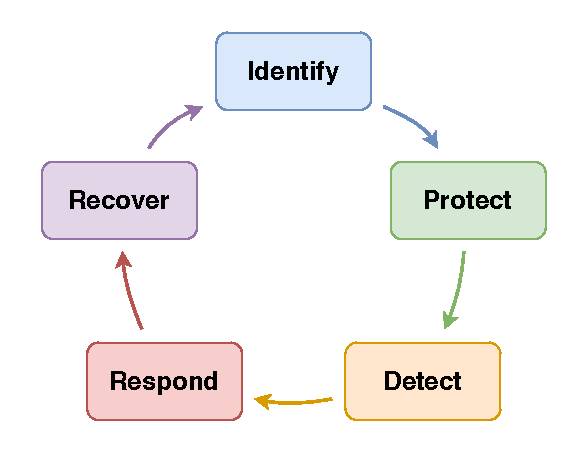
\includegraphics[width=.4\linewidth]{figures/thesis/intro/security.drawio.pdf}
%     \caption*{The security life-cycle \footcite{nationalinstituteofstandardsandtechnology_NISTCybersecurityFramework_2024}.}
%   \end{figure}
% \end{frame}

% \begin{frame}{The Need for Collaboration}
%   \centering
%   \foreach \i in {1,...,4} {%
%     \includegraphics<\i>[width=.9\textwidth]{figures/thesis/intro/collab/collab-\i.drawio.pdf}%
%   }
% \end{frame}

\begin{frame}{Machine Learning for Intrusion Detection}
  % \begin{columns}
  %   \begin{column}{.6\textwidth}
  %     \sntoptions{block=fill}
  %     \begin{block}{Intrusion Detection System (IDS)}
  %       \medskip
  %       IDSs monitor the behavior of a system to detect malicious activities.
  %     \end{block}
  %   %   \begin{itemize}
  %   %     \item Collaboration pushed by:
  %   %     \begin{itemize}[<+->]
  %   %       \item common interest (\eg, inter-SOCs\footnotemark);
  %   %       \item national agencies (\eg, NIST, ENISA, ANSSI);
  %   %       \item regulation (\eg, private-public information sharing in NIS2).
  %   %     \end{itemize}
  %   %   \end{itemize}
  %   \end{column}
  \begin{columns}
    \column{.4\textwidth}
    \centering
    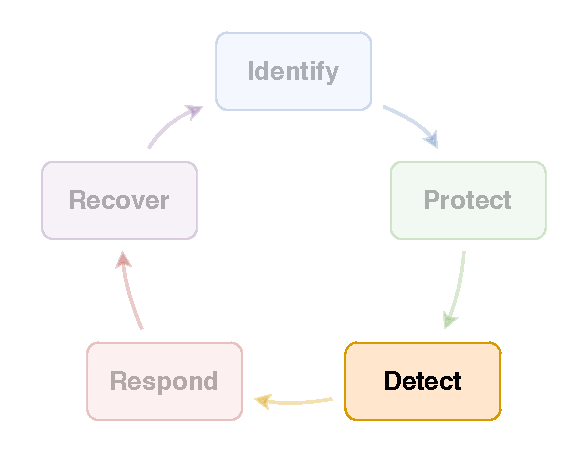
\includegraphics[width=\linewidth]{figures/thesis/intro/security-focus.drawio.pdf}
  
    \column{.6\textwidth}
    \textbf{Solved problem?}
    \begin{itemize}[<+->]
      \item Deep Learning (DL) offers very high performance\dots{} \onslide<+->\emph{on public datasets at least}.
      \item Various strategies: \alert<+->{supervised}, unsupervised, semi-supervised, reinforcement learning, \etc.
    \end{itemize}
  \end{columns}

\end{frame}




\begin{frame}{IDS Deployment Challenges}
  % \stepcounter{beamerpauses}
  % \bigskip
  % \only<+>{}%
  % \begin{itemize}[<+->]
  %   \item Over-representation of Deep Learning, offering high performance (DL)\dots{} \onslide<+->\emph{on public datasets at least}.
  %   \item Various strategies: \alert<+->{supervised}, unsupervised, semi-supervised, reinforcement learning, \etc.
  % \end{itemize}
    % \item Great performance with Deep Learning (DL)\dots{}
    % \onslide<+->
    % \emph{on public datasets at least}.
  % \end{itemize}
  % \bigskip
  
  \onslide<+->
  \begin{columns}
    \begin{column}{0.5\textwidth}
      %\bigskip
      \begin{block}{Challenges of local training}
        \begin{itemize}
          \item not enough labelled data;
          \item risk of local bias or skewed data distribution.
          % \item inefficient against new attacks, especially \alert{supervised} approaches.
        \end{itemize}
      \end{block}
      \onslide<+->{
      \begin{block}{Push for collaboration}
        \begin{itemize}
          \item common interest (\eg, inter-SOCs\footnotemark);
          \item national agencies (\eg, NIST, ANSSI);
          \item regulation (\eg, private-public information sharing in NIS2).
        \end{itemize}
      \end{block}
      }
    \end{column}
    \onslide<1->
    \begin{column}{0.5\textwidth}
      \begin{figure}
        \centering
        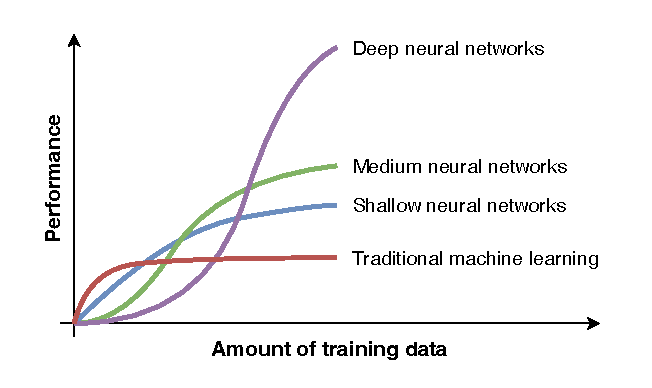
\includegraphics[width=\linewidth]{figures/thesis/intro/ml-perf}
      \end{figure}
    \end{column}
  \end{columns}
\end{frame}

\begin{frame}{Data Sharing to the Rescue?}
% TODO:
% pas assez de données, faisons un pot commun !
% oui mais non :
% - confidentialité des données 
% - confiance dans le point de collecte
% - confiance dnas le processus d'apprentissage
% - pas de modèle de detection sans serveur
\begin{columns}
  \begin{column}{0.5\textwidth}
    \centering
    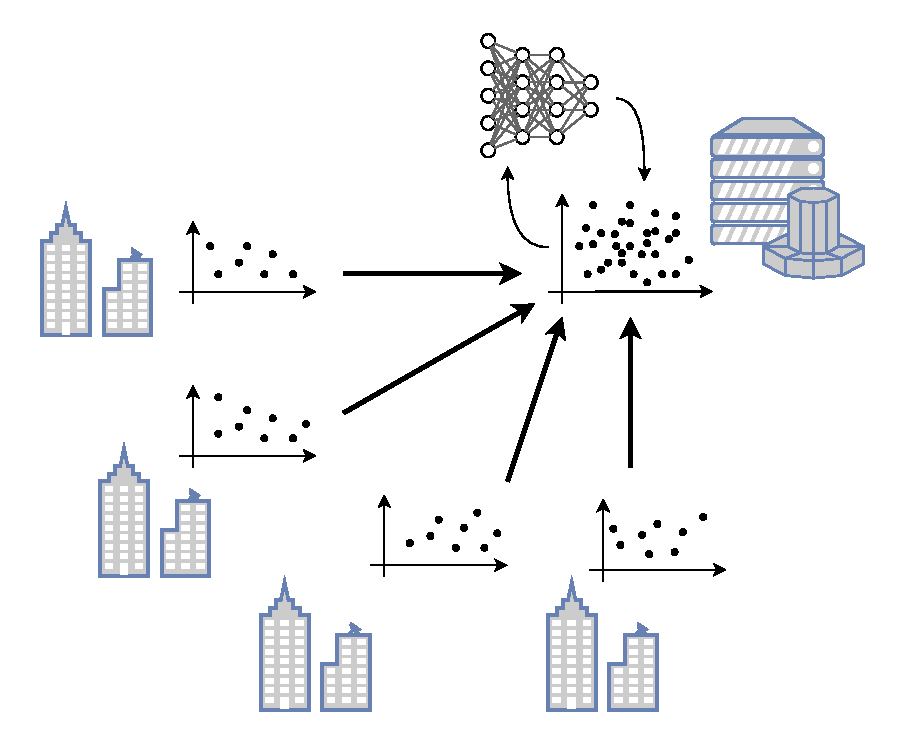
\includegraphics[width=\linewidth]{figures/thesis/intro/collab.pdf}
  \end{column}
  \begin{column}{0.5\textwidth}
    \textbf{Let's pool our data!}\pause{} \textbf{Although\dots}
    \begin{itemize}
      \item Privacy concerns.
      \item Lack of trust in the data holder.
      \item Lack of trust in the learning process.
      %\item Lack of incentives.
      \item \dots
    \end{itemize}
  \end{column}
\end{columns}
\end{frame}

\begin{frame}{Scaling Intrusion Detection}
  \begin{columns}
    \column{.45\textwidth}
    \begin{block}{Federated Learning (FL)}
      \begin{itemize}
        \item Recent-\textit{ish} distributed ML paradigm~\autocite{mcmahan_Communicationefficientlearningdeep_2017}.
        \item Clients train a common model without sharing their training data.
        \item \alert{Privacy-preserving}: model sharing partially prevents data leakage.
      \end{itemize}
    \end{block}

    \column{.55\textwidth}
    \begin{figure}
      \centering
      % \foreach \i in {1,...,7} {%
      %   \includegraphics<\i>[width=\linewidth]{./figures/thesis/intro/fl/\i.pdf}%
      % }
      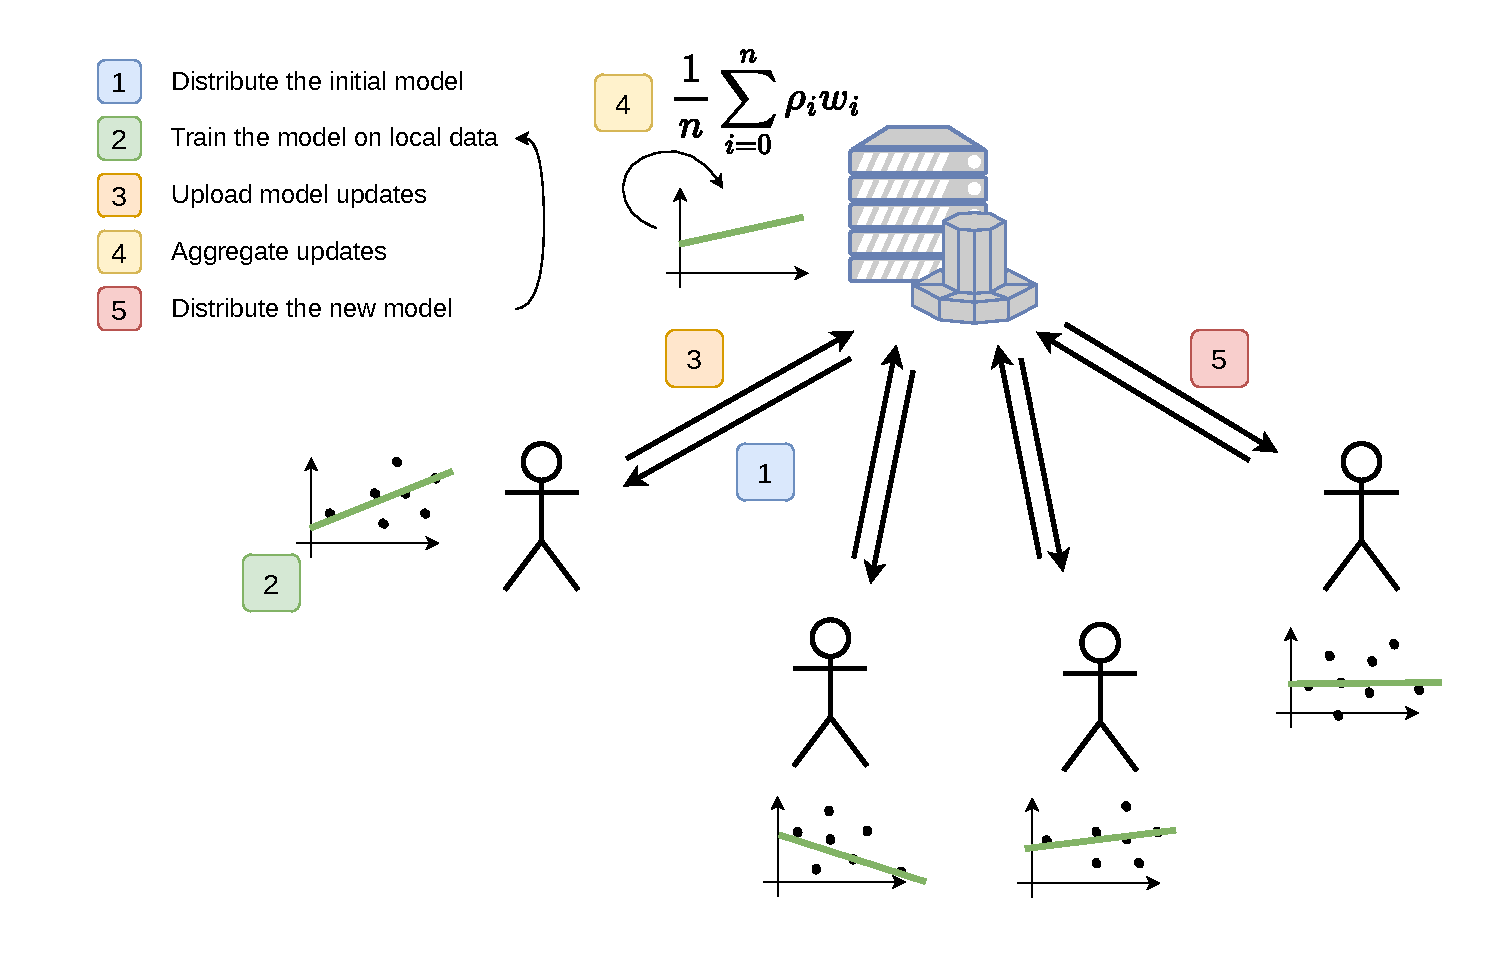
\includegraphics[width=\linewidth]{./figures/feditn/intro/fl.drawio.pdf}
      \caption{Typical FL workflow}
  \end{figure}
  \end{columns}

  \footcite*{mcmahan_Communicationefficientlearningdeep_2017}
\end{frame}


% \begin{frame}{FL Fundamentals}
%   \begin{figure}
%     \centering
%     \foreach \i in {1,...,7} {%
%       \includegraphics<\i>[width=.75\linewidth]{./figures/thesis/intro/fl/\i.pdf}%
%     }
%     \caption{Typical FL workflow, applied to NIDSs.}
%   \end{figure}
% \end{frame}


\section{Federated Learning for Intrusion Detection}

\begin{frame}{PhD Thesis}
  \begin{block}{Improving Intrusion Detection in Distributed Systems with Federated Learning}
    \begin{itemize}
      \item \alert{Goal}: Can federated learning realistically be used to as a mean of collaboration between organizations for intrusion detection?
      \item Supervised by Yann Busnel, advised by Fabien Autrel and Marc-Oliver Pahl.
      \item Hosted at IMT Atlantique/IRISA with industry and academic funding (Chair CyberCNI).
      %\item Defended on October 7\textsuperscript{th}, 2024. Jury: Vincent Nicomette (INSA Toulouse), Anne-Marie Kermarrec (EPFL), Éric Totel (TSP), Sonia Ben Mokhtar (CNRS), Pierre-François Gimenez (Inria), Yann Busnel, Fabien Autrel, and Marc-Oliver Pahl (IMT Atlantique).
      \item Multiple publications in international journals~\autocite{lavaur_tnsm_2022,lavaur_cose_2025}, conferences~\autocite{lavaur_icdcs_demo_2024,lavaur_radar_2024} and workshops~\autocite{lavaur_ares_bass_2024}, as well as international tutorials~\autocite{lavaur_nof_tuto_2023,lavaur_icdcs_tuto_2024,lavaur_icdcs_tuto_2025} and national venues~\autocite{lavaur_cesar_2022,lavaur_algotel_2025}.
      % \item Keywords: federated learning, collaborative intrusion detection, machine learning, cybersecurity, distributed systems.
    \end{itemize}
  \end{block}

  \tikz[overlay,remember picture]{
    \node[anchor=south east, xshift=-1em, yshift=.5em] at (current page.south east) {%
      \raisebox{-0.5\height}{
\includegraphics[height=1.2cm]{figures/thesis/logos/cybercni.pdf}}%
      \hspace{1em}\raisebox{-0.5\height}{
\includegraphics[height=1cm]{figures/thesis/logos/imta.png}}%
      \hspace{.7em}\raisebox{-0.5\height}{
\includegraphics[height=1cm]{figures/thesis/logos/irisa.jpg}}%
    }
  }
\end{frame}

\newcommand<>\highlightbox[2]{%
  \alt#3{\makebox[\dimexpr\width-2\fboxsep]{\colorbox{#1}{#2}}}{#2}%
}
\definecolor{chal-poison}{HTML}{1e78b4}\newcommand{\chpoison}[2][1-]{\highlightbox<#1>{chal-poison!50}{#2}}
\definecolor{chal-qual}{HTML}{ff7f0f}\newcommand{\chqual}[2][1-]{\highlightbox<#1>{chal-qual!50}{#2}}
\definecolor{chal-decent}{HTML}{2da02d}\newcommand{\chdecent}[2][1-]{\highlightbox<#1>{chal-decent!50}{#2}}
\definecolor{chal-feat}{HTML}{d62727}\newcommand{\chfeat}[2][1-]{\highlightbox<#1>{chal-feat!50}{#2}}
\definecolor{chal-hetero}{HTML}{9567bd}\newcommand{\chhetero}[2][1-]{\highlightbox<#1>{chal-hetero!50}{#2}}
\definecolor{chal-unknown}{HTML}{8d574b}\newcommand{\chunknown}[2][1-]{\highlightbox<#1>{chal-unknown!50}{#2}}
\definecolor{chal-transfer}{HTML}{e377c3}\newcommand{\chtransfer}[2][1-]{\highlightbox<#1>{chal-transfer!50}{#2}}
\definecolor{chal-comm}{HTML}{7f7f7f}\newcommand{\chcomm}[2][1-]{\highlightbox<#1>{chal-comm!50}{#2}}



% \subsection[\slr Systematic Literature Review]{\texorpdfstring{\circled{contrib/slr}{S}~Federated Intrusion Detection Systems}{Federated Intrusion Detection Systems}}

% \begin{frame}[plain]
%   \subsectionpage
  
%   \footcite*{lavaur_tnsm_2022}
%   \footcite*{lavaur_cesar_2022}
%   \footcite*{lavaur_icdcs_demo_2024}
% \end{frame}

\begin{frame}{Case Study}
  \bigskip
  \textbf{Collaborating with Federated Intrusion Detection Systems (FIDSs)}:
  \begin{itemize}[<+->]
    \item Each organization has its own NIDS\footnotemark{} and monitors an information system.
    \item Objective: improve their local detection performance.
    \item Means: \alert{expert knowledge} (\ie, datasets) and \alert{computing resources} (\ie, model training).
  \end{itemize}
  % \only<1>{\footnotetext[1]{Network Intrusion Detection System}}
  \onslide<+->
  \begin{columns}
    \column{.5\textwidth}
    \textbf{A cross-silo use case}~\autocite{kairouz_AdvancesOpenProblems_2021}:
    \begin{itemize}
      \item few clients (\ie, 10--100);
      \item substantial amount of data, high heterogeneity;
      \item high availability, significant computing resources.
    \end{itemize}

    \onslide<+->
    \column{.5\textwidth}
    \vspace{-1.5em}
    \begin{figure}
      \centering
      \resizebox{.8\linewidth}{!}{\input{figures/thesis/intro/year_histogram.pgf}}
      \caption{Publications on FL \& IDS (until 2024-04). 1600+ results on Scopus in 2026-02.}
    \end{figure}
  \end{columns}

  \alt{\footcite*{kairouz_AdvancesOpenProblems_2021}}{\blankfootnote{\newline}}
  % \begin{figure}
  %   \centering
  %   \makebox[\textwidth][c]{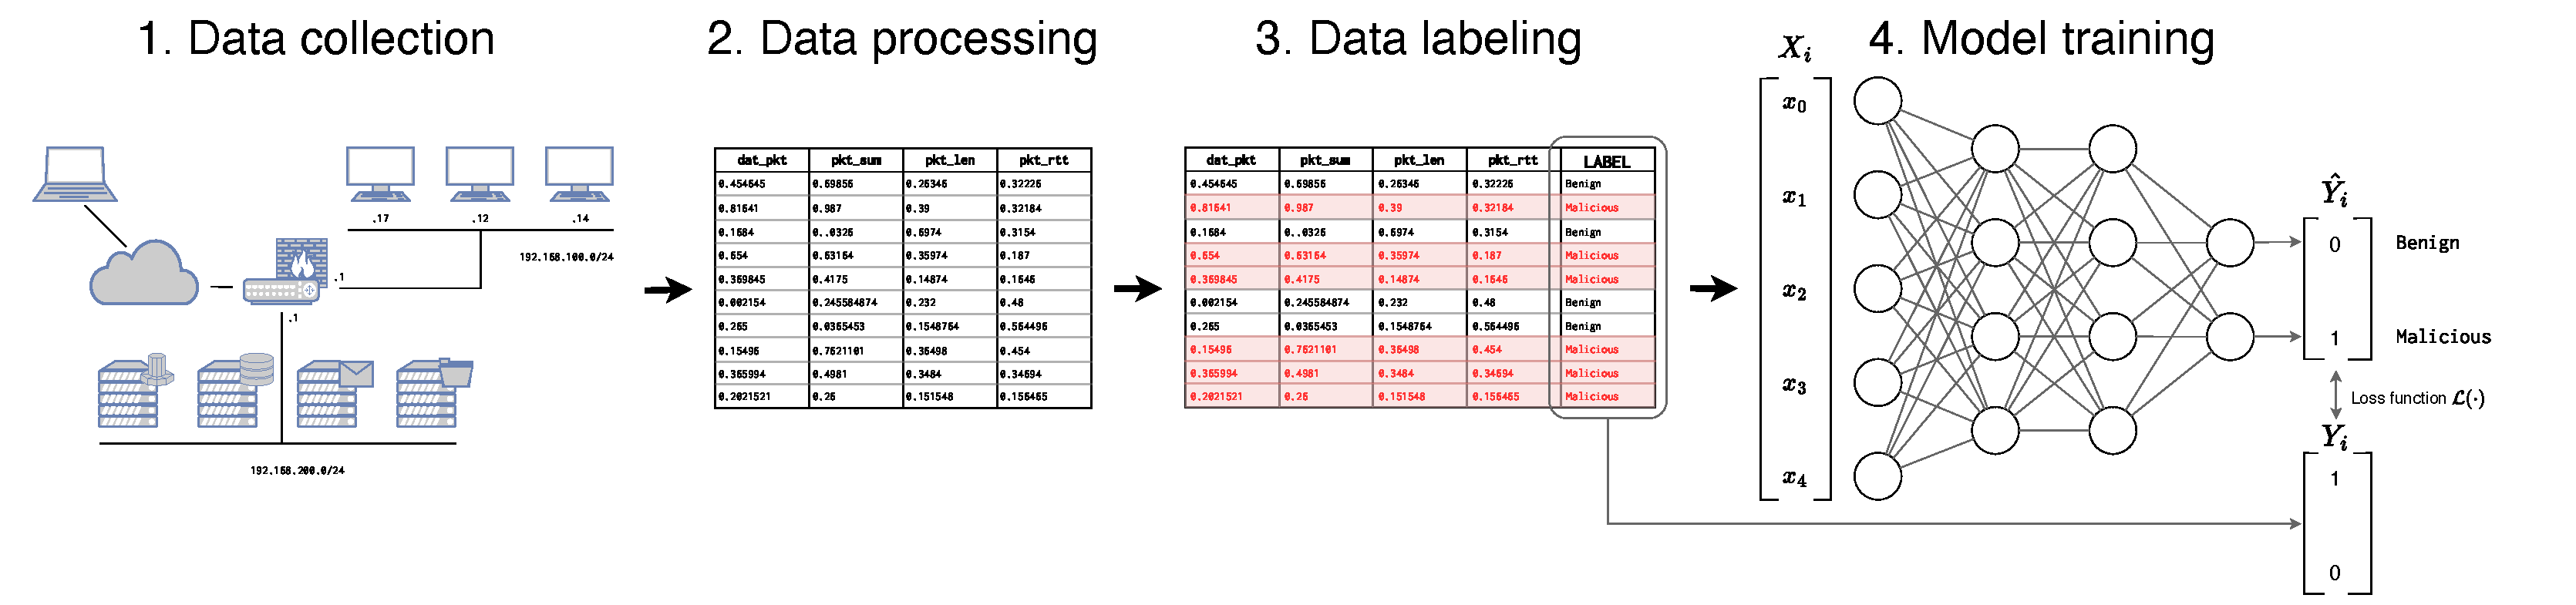
\includegraphics[width=.9\textwidth]{figures/thesis/intro/mlp-workflow.pdf}}
  %   \caption{Typical workflow for ML-based NIDSs.}
  % \end{figure}
\end{frame}

% \begin{frame}{Systematic Literature Review}
  
%   \begin{columns}
%     \begin{column}{.45\textwidth}
%       % \textbf{Systematic Literature Review (SLR)}~\autocite{lavaur_tnsm_2022}
%       % \begin{itemize}
%       %   \item Booming topic over the last 4--5 years.
%       %   \item Very heterogeneous venues and communities.
%       % \end{itemize}

%       \textbf{Challenges from the Literature}~\autocite{lavaur_tnsm_2022}
%       \begin{itemize}[<+->]
%         \item \textit{Functionality}: \chqual[6-]{performance}, \chhetero[6-]{heterogeneity}, \chtransfer[6-]{transferability}, self-defense, and self-healing.
%         \item \textit{Deployment}: \chunknown[6-]{adaptability} and \chdecent[6-]{scalability}.
%         \item \textit{Security and reliability}: \chpoison[6-]{security}, privacy, \chpoison[6-]{trust}, and reputation.
%         \item \textit{Experimentation}: evaluation.
%       \end{itemize}
%     \end{column}
%     \begin{column}{.55\textwidth}
%       \only<5-6>{%
%         \begin{figure}
%           \centering
%           \resizebox{\linewidth}{!}{\input{figures/thesis/intro/challenges_histogram.pgf}}
%           \caption{Challenges addressed by the literature (until 2024-04).}
%         \end{figure}
%       }
%       \only<7>{%
%         \begin{figure}
%           \centering
%           \resizebox{\linewidth}{!}{\input{figures/thesis/intro/year_histogram.pgf}}
%           \caption{Publications on FL \& IDS (until 2024-04). 1600+ results on Scopus in 2026-02.}
%         \end{figure}
%       }
%     \end{column}
%   \end{columns}

%   \footcite*{lavaur_tnsm_2022}
% \end{frame}


\newcommand<>\mktransparent[2]{\alt#3{\texttransparent{#1}{#2}}{#2}}

\begin{frame}{Addressed Challenges}
  
  \begin{columns}
    \begin{column}{.5\textwidth}
      \begin{figure}
        \centering
        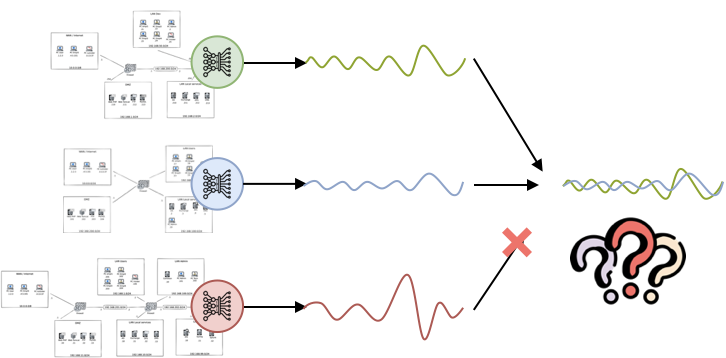
\includegraphics[width=\linewidth]{figures/thesis/intro/heterogeneity.png}
        \caption{Heterogeneity headaches.}
      \end{figure}
    \end{column}

    \begin{column}{.5\textwidth}
      \mktransparent<2->{0.5}{%
      \textbf{Challenge I}: \textit{Too much heterogeneity leads to poor performance\dots}~\autocite{lavaur_icdcs_demo_2024}
      }

      \medskip
      \mktransparent<1,3>{0.5}{%
      \textbf{Challenge II}: \textit{Difficult to identify malicious contributions when models are different\dots}
      }
      
      \medskip
      \mktransparent<1-2>{0.5}{%
      \textbf{Challenge III}: \textit{No representative dataset of heterogeneous distributed intrusion detection\dots}~\autocite{lavaur_cesar_2022}
      }
    \end{column}
  \end{columns}

  \only<1>{\footcite*{lavaur_icdcs_demo_2024}}
  \only<2>{\blankfootnote{\newline}}
  \only<3>{\footcite*{lavaur_cesar_2022}}
  
\end{frame}


\begin{frame}[t]{Contributions Summary}
  \centering%
  \vspace{-.2cm}
  \foreach \i in {1,...,9} {%
    \includegraphics<\i>[width=1.1\linewidth, center,trim={0 0 0 1.2cm}, clip]{./figures/thesis/intro/metro/\i.pdf}%
  }
  % \includegraphics<10->[width=1.1\linewidth, center]{./figures/thesis/intro/metro/10.pdf}%

  % \only<11>{
  %   \tikz[overlay, remember picture,
  %     shift=(current page.south west),
  %     x=(current page.south east),
  %     y=(current page.north west)
  %   ]{
  %     % Optional help grid lines
  %     %\draw[step=.1, opacity=0.3, thick, red] (0,0) grid (1,1);
      
  %     \node[align=left, anchor=south west] at (.025, .05) {\begin{minipage}{.8\textwidth}
  %       \tableofcontents
  %     \end{minipage}};
  %   }
  % }

\end{frame}

\newtcolorbox{taxobox}[1][]{
  enhanced,
  colback=sntPurple!5,
  colbacktitle=sntPurple,
  coltitle=white,
  sharp corners,
  frame hidden,
  boxrule=0pt,
  fontupper=\small,
  fonttitle=\centering\bfseries\scshape,
  after title app=\strut,
  height=3.5cm,
  title=#1
}

\subsection[\eiffel Assessment \& \texttt{eiffel}]{\texorpdfstring{\eiffel Assessing the Impact of Label-Flipping Attacks}{Assessing the Impact of Label-Flipping Attacks}}


% \begin{frame}[plain]
%   \subsectionpage

%   \footcite*{lavaur_ares_bass_2024}
%   \footcite*{lavaur_cose_2025}
% \end{frame}


\begin{frame}{The Problem of Poisoning Attacks}
  \stepcounter{beamerpauses}
  \begin{columns}
    \column{.5\textwidth}
      \begin{block}{Definition}
        Manipulation of the training data or model updates cause unwanted behaviors in the aggregated model.
      \end{block}
      \onslide<+->{
      \begin{block}{Unclear impact in FIDSs}
        \begin{itemize}
          \item Big systematic study on characterizing label-flipping attacks in FIDSs~\autocite{lavaur_cose_2025}.
          \item Scope: predictability, hyperparameter dependencies, impact characterization and detection.
          \item Reproducible evaluation framework (\texttt{eiffel}).
        \end{itemize}
      \end{block}
      }
      
    \column{.5\textwidth}
      \onslide<1->{
      \begin{figure}
        \centering
        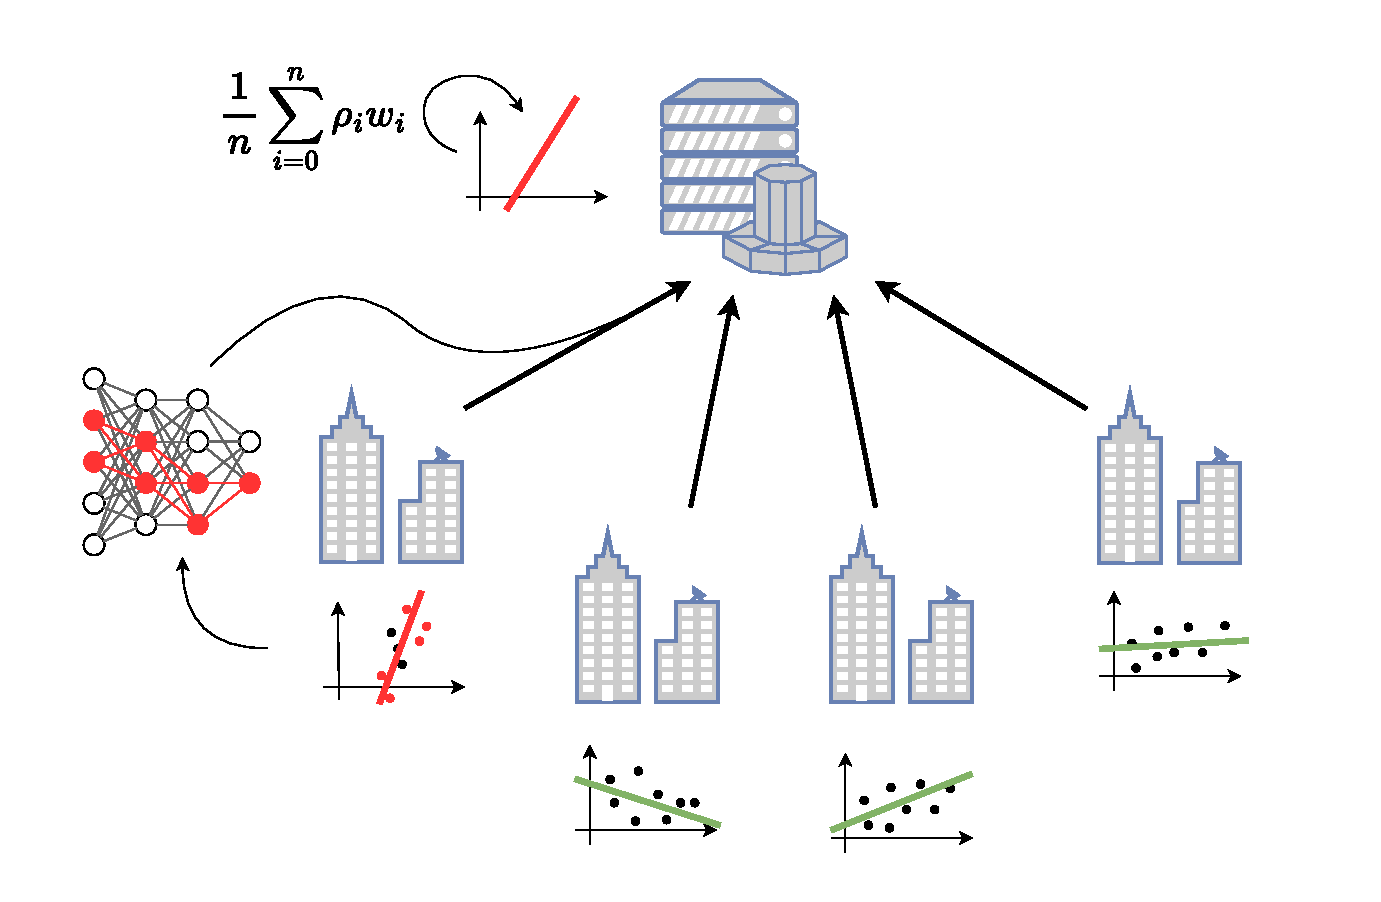
\includegraphics[width=\textwidth,trim={0 1cm 0 1cm},clip]{figures/thesis/assessment/poisoning/6.pdf}
        \caption{Poisoning attacks on FL.}
      \end{figure}}
  \end{columns}

  \alt<2->{\footcite*{lavaur_cose_2025}}{\blankfootnote{\newline}}
\end{frame}

% \begin{frame}{Characterizing Poisoning Attacks}
%   \centering
%   \begin{tcolorbox}[
%     enhanced,
%     colback=sntBlue,
%     boxrule=0pt,
%     frame hidden,
%     fontupper=\large\bfseries,
%     hbox,
%     colupper=white,
%   ]
%     Poisoning attacks
%   \end{tcolorbox}
  
%   \vspace{1em}
  
%   \setlength{\leftmargini}{5pt}
%   \begin{columns}
%     \pause\column{.33\textwidth}
%     \begin{taxobox}[Component]
%       \begin{itemize}
%         \item Data poisoning (\eg, \alert<5>{label-flipping}, clean-label)
%         \item Model poisoning (\eg, gradient boosting)
%       \end{itemize}
%     \end{taxobox}

%     \pause\column{.33\textwidth}
%     \begin{taxobox}[Objective]
%       \begin{itemize}
%         \item Untargeted: impact model performance
%         \item Targeted: modify behavior for specific samples
%       \end{itemize}
%     \end{taxobox}

%     \pause\column{.33\textwidth}
%     \begin{taxobox}[Proportion]
%       \begin{itemize}
%         \item Single attacker
%         \item Colluding attackers: multiple coordinated adversaries
%       \end{itemize}
%     \end{taxobox}
%   \end{columns}
% \end{frame}
  

% \begin{frame}{Scope of the Study}
%   \textbf{Existing studies}
%   \begin{itemize}
%     \item Often partial, focusing on challenging a specific defense mechanism.
%     \item Lack of reproducibility and comparability (different datasets, models, and attacks).
%     \item No targeted attacks binary classification.
%   \end{itemize}

%   % \pause
%   % \textbf{Research Questions}
%   % \begin{enumerate}
%   %   \item Is the behavior of poisoning attacks predictable?
%   %   \item Do hyperparameters influence the impact of poisoning attacks?
%   %   \item Are IDS backdoors realistic using label-flipping attacks?
%   %   \item Is there a critical threshold where label-flipping attacks begin to impact performance?
%   %   \item \alert<3>{Is gradient similarity enough to detect label-flipping attacks?}
%   % \end{enumerate}
% \end{frame}


\begin{frame}{Similarity-based Mitigation against Heterogeneity}

  \begin{columns}
    \begin{column}{.45\textwidth}
      \begin{itemize}[<+->]
        \item Known technique to detect poisoning attacks~\autocite{tolpegin_DataPoisoningAttacks_2020}.
        \item High heterogeneity makes it harder to detect attackers.
      \end{itemize}
    \end{column}

    \begin{column}{.55\textwidth}
      \begin{figure}
        \centering
        \foreach \i in {1,...,3}{%
          \includegraphics<\i>[width=\textwidth,trim={1cm 3cm 1cm 3cm},clip]{figures/thesis/assessment/similarity-untargeted-colluding-cicids-\i.pdf}%
        }
        \caption{PCA projection of the gradients in 2D (CICIDS).}
      \end{figure}
    \end{column}
  \end{columns}

  \footcite*{tolpegin_DataPoisoningAttacks_2020}

\end{frame}

% \begin{frame}{Highlights}
%   % \begin{enumerate}
%   %   \item A \emph{deeper} understanding of the behavior of label-flipping attacks in FL-based CIDSs.

%   \begin{block}{Detection using similarity is not enough}
%     Increasing \alert{heterogeneity} removes the baseline necessary to discriminate contributions
%   \end{block}

%   \pause
%   \begin{block}{Good generalizability defeat tageted poisoning}
%     Feature-overlap between classes and model's \alert{generalization} capabilities limit the attacker's ability to select specific attack classes.
%   \end{block}

%   \pause
%   \begin{block}{High hyperparameter depdendencies}
%     Hyperparameter choices have a significant impact on the attack's impact and \alert{propagation}.
%   \end{block}

%   \footcite*{lavaur_cose_2025}
  
% \end{frame}
\subsection[\radar~\texttt{RADAR}]{\texorpdfstring{\radar Fighting Byzantine Contributions in Heterogeneous Settings}{Fighting Byzantine Contributions in Heterogeneous Settings}}

% \begin{frame}[plain]
%   \subsectionpage

%   \footcite*{lavaur_radar_2024}
% \end{frame}


\begin{frame}{Handling Byzantine Contributions in Heterogeneous Settings}
  \stepcounter{beamerpauses}
  \begin{columns}
    \column{.5\textwidth}
    \textbf{Working assumptions}
    \begin{itemize}
      \item Multiple organizations using a FIDS.
      \item Partial heterogeneity in the datasets: different data distributions but existing similarities.
    \end{itemize}
  
    \onslide<+(1)->{
    \textbf{Byzantine contributions}
    \begin{itemize}[<+->]
      \item data quality issues (\eg, labelling, noise);
      \item distribution mismatches; and
      \item adversaries\onslide<+->{, \alert{possibly colluding}}.
    \end{itemize}
    }

    \column{.5\textwidth}
    \onslide<2->
    \begin{figure}
      \centering
      \includegraphics<1-4>[width=\textwidth]{figures/radar-eval/setup/partition.pdf}%
      \includegraphics<5->[width=\textwidth]{figures/radar-eval/setup/poisoning.pdf}%
    \end{figure}
    
  \end{columns}  

\end{frame}

% \begin{frame}{Problem Statement}
%   \begin{block}{Quality Assessment in Heterogeneous Settings}
%     For $n$ participants $p_i$ and their local datasets $d_i$ of unknown similarity, each participant uploads a model update $w_i^r$ at each round $r$. Given $P = \{ p_1, p_2, \dots, p_n \} $ and $W = \{ w_1^r, w_2^r, \dots, w_n^r \} $, how can one assess the quality of each participant’s contribution without making assumptions on the data distribution across the datasets $d_i$?
%   \end{block}
% \end{frame}


% \begingroup  % Remove the Author for this slide, as the citations step on the footer.
% \setbeamertemplate{frame footer}{}
% \begin{frame}{Existing Solutions}

%   \begin{columns}[T]
    
%     \begin{column}{.33\textwidth}
%       \footnotesize\centering
%       \textbf{Server-side evaluation}~\autocite{zhou_DifferentiallyPrivateFederated_2022}

%       \begin{figure}
%         \centering
%         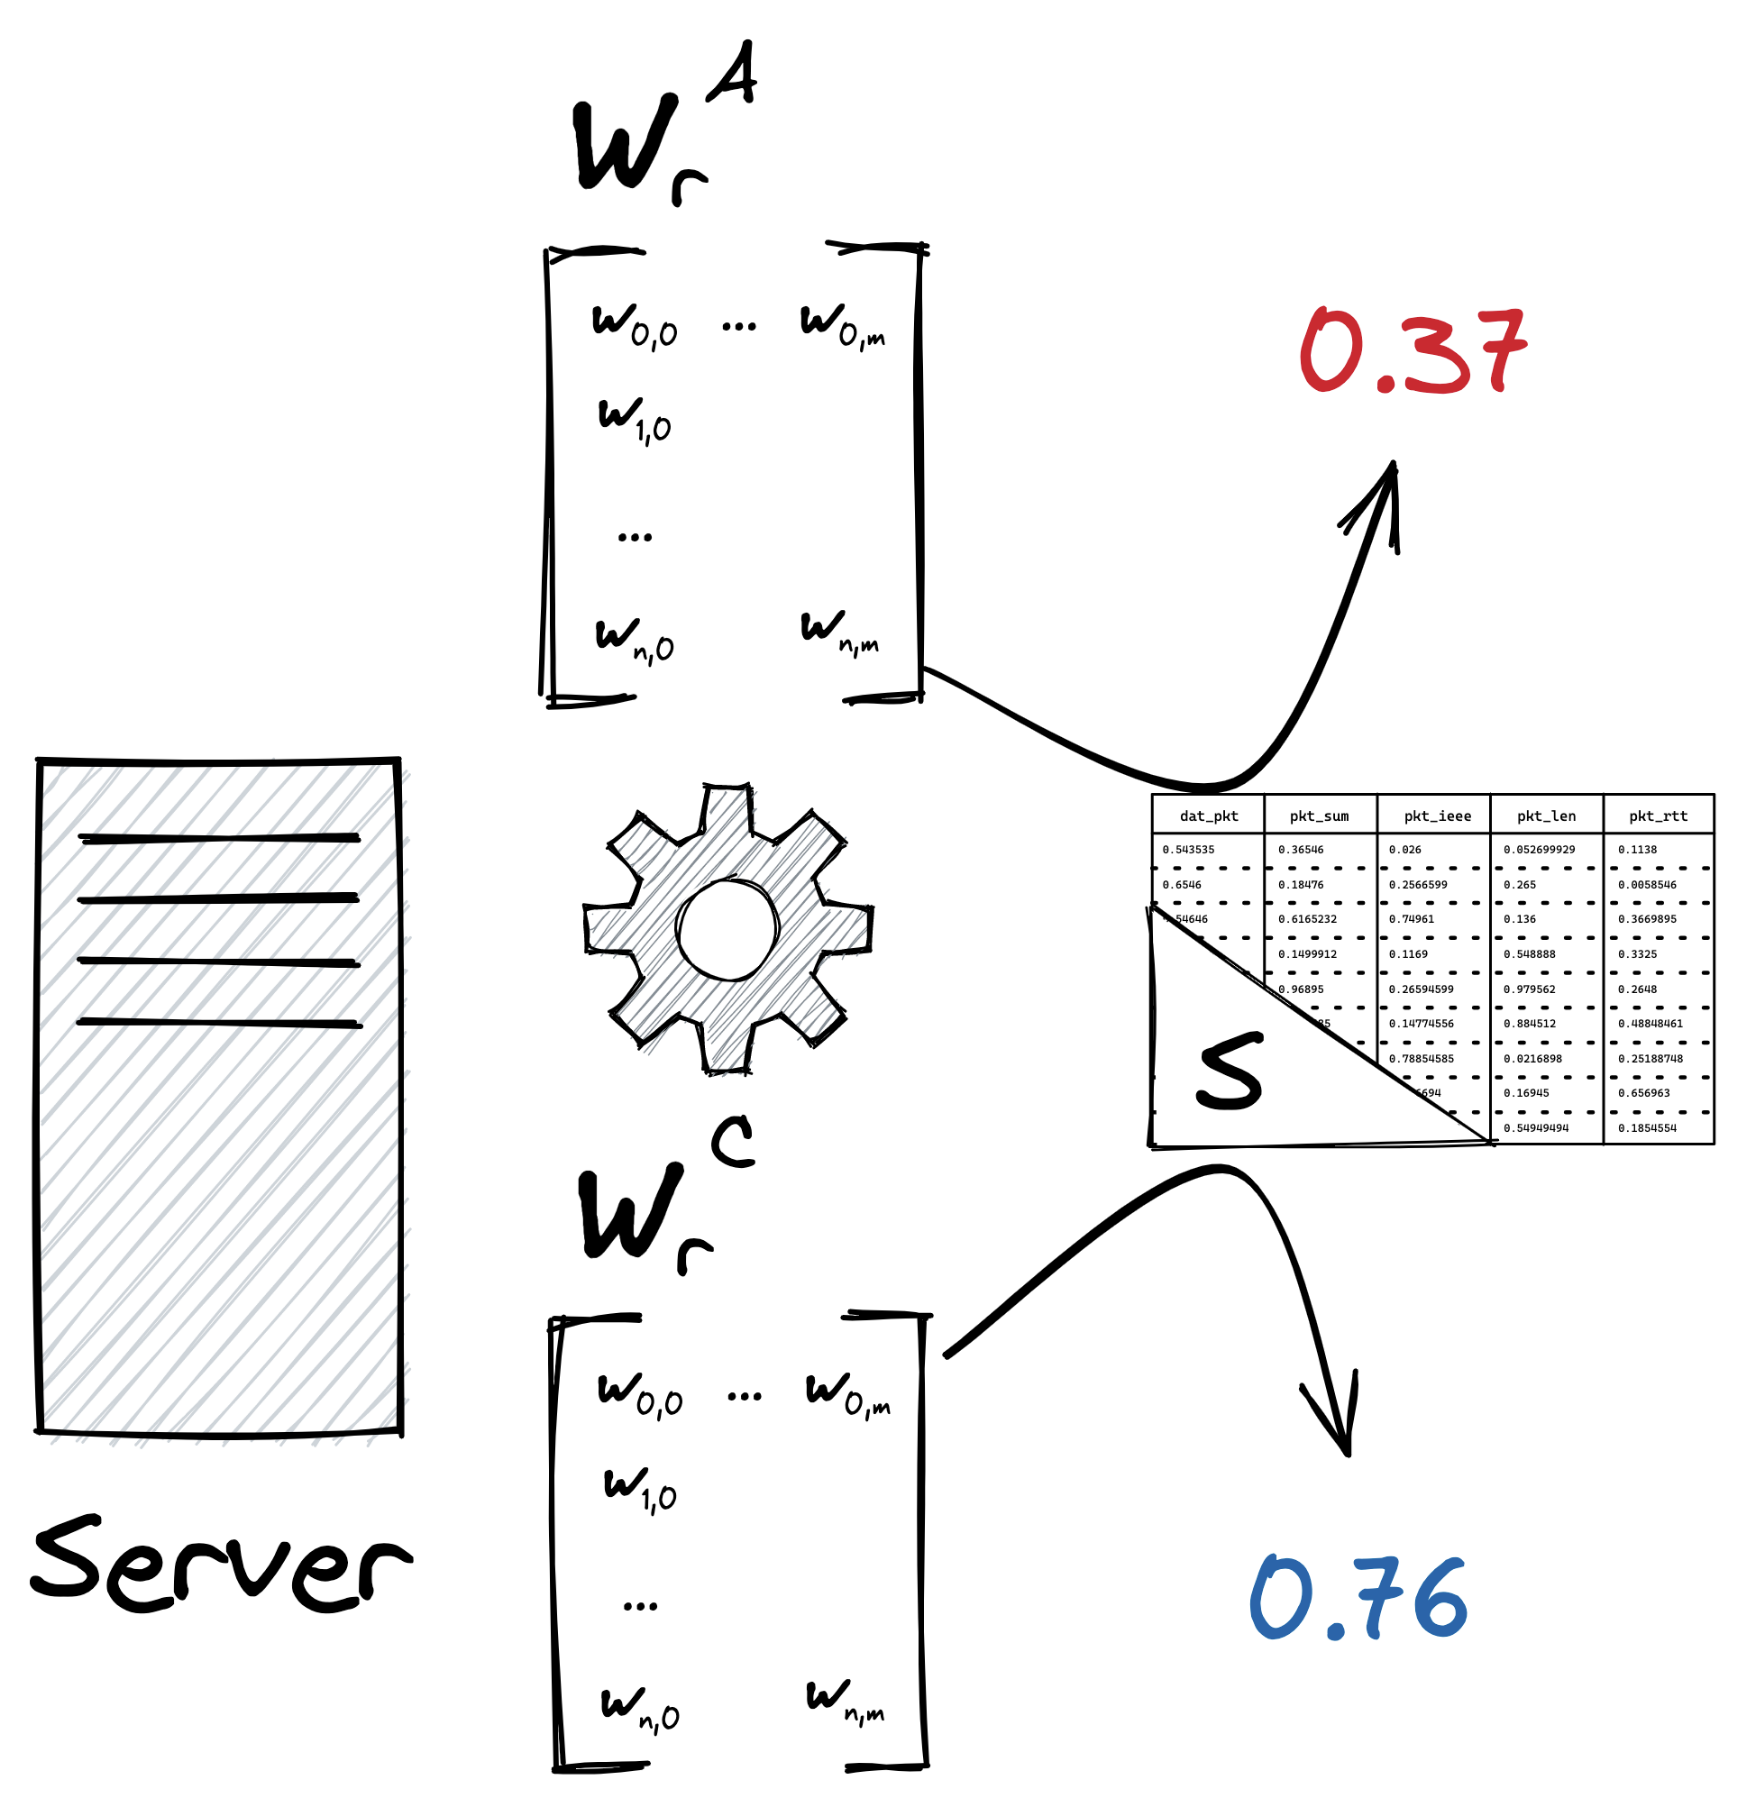
\includegraphics[height=.36\textheight]{figures/thesis/radar/server-side-eval}
%       \end{figure}

%       \begin{itemize}\footnotesize
%         \item Only applicable in IID settings.
%         \item Single source of truth.
%       \end{itemize}
%     \end{column}

%     \onslide<2->{%
%       \begin{column}{.33\textwidth}
%         \footnotesize\centering
%         \textbf{Server-side comparison}~\autocite{briggs_Federatedlearninghierarchical_2020}

%         \begin{figure}
%           \centering
%           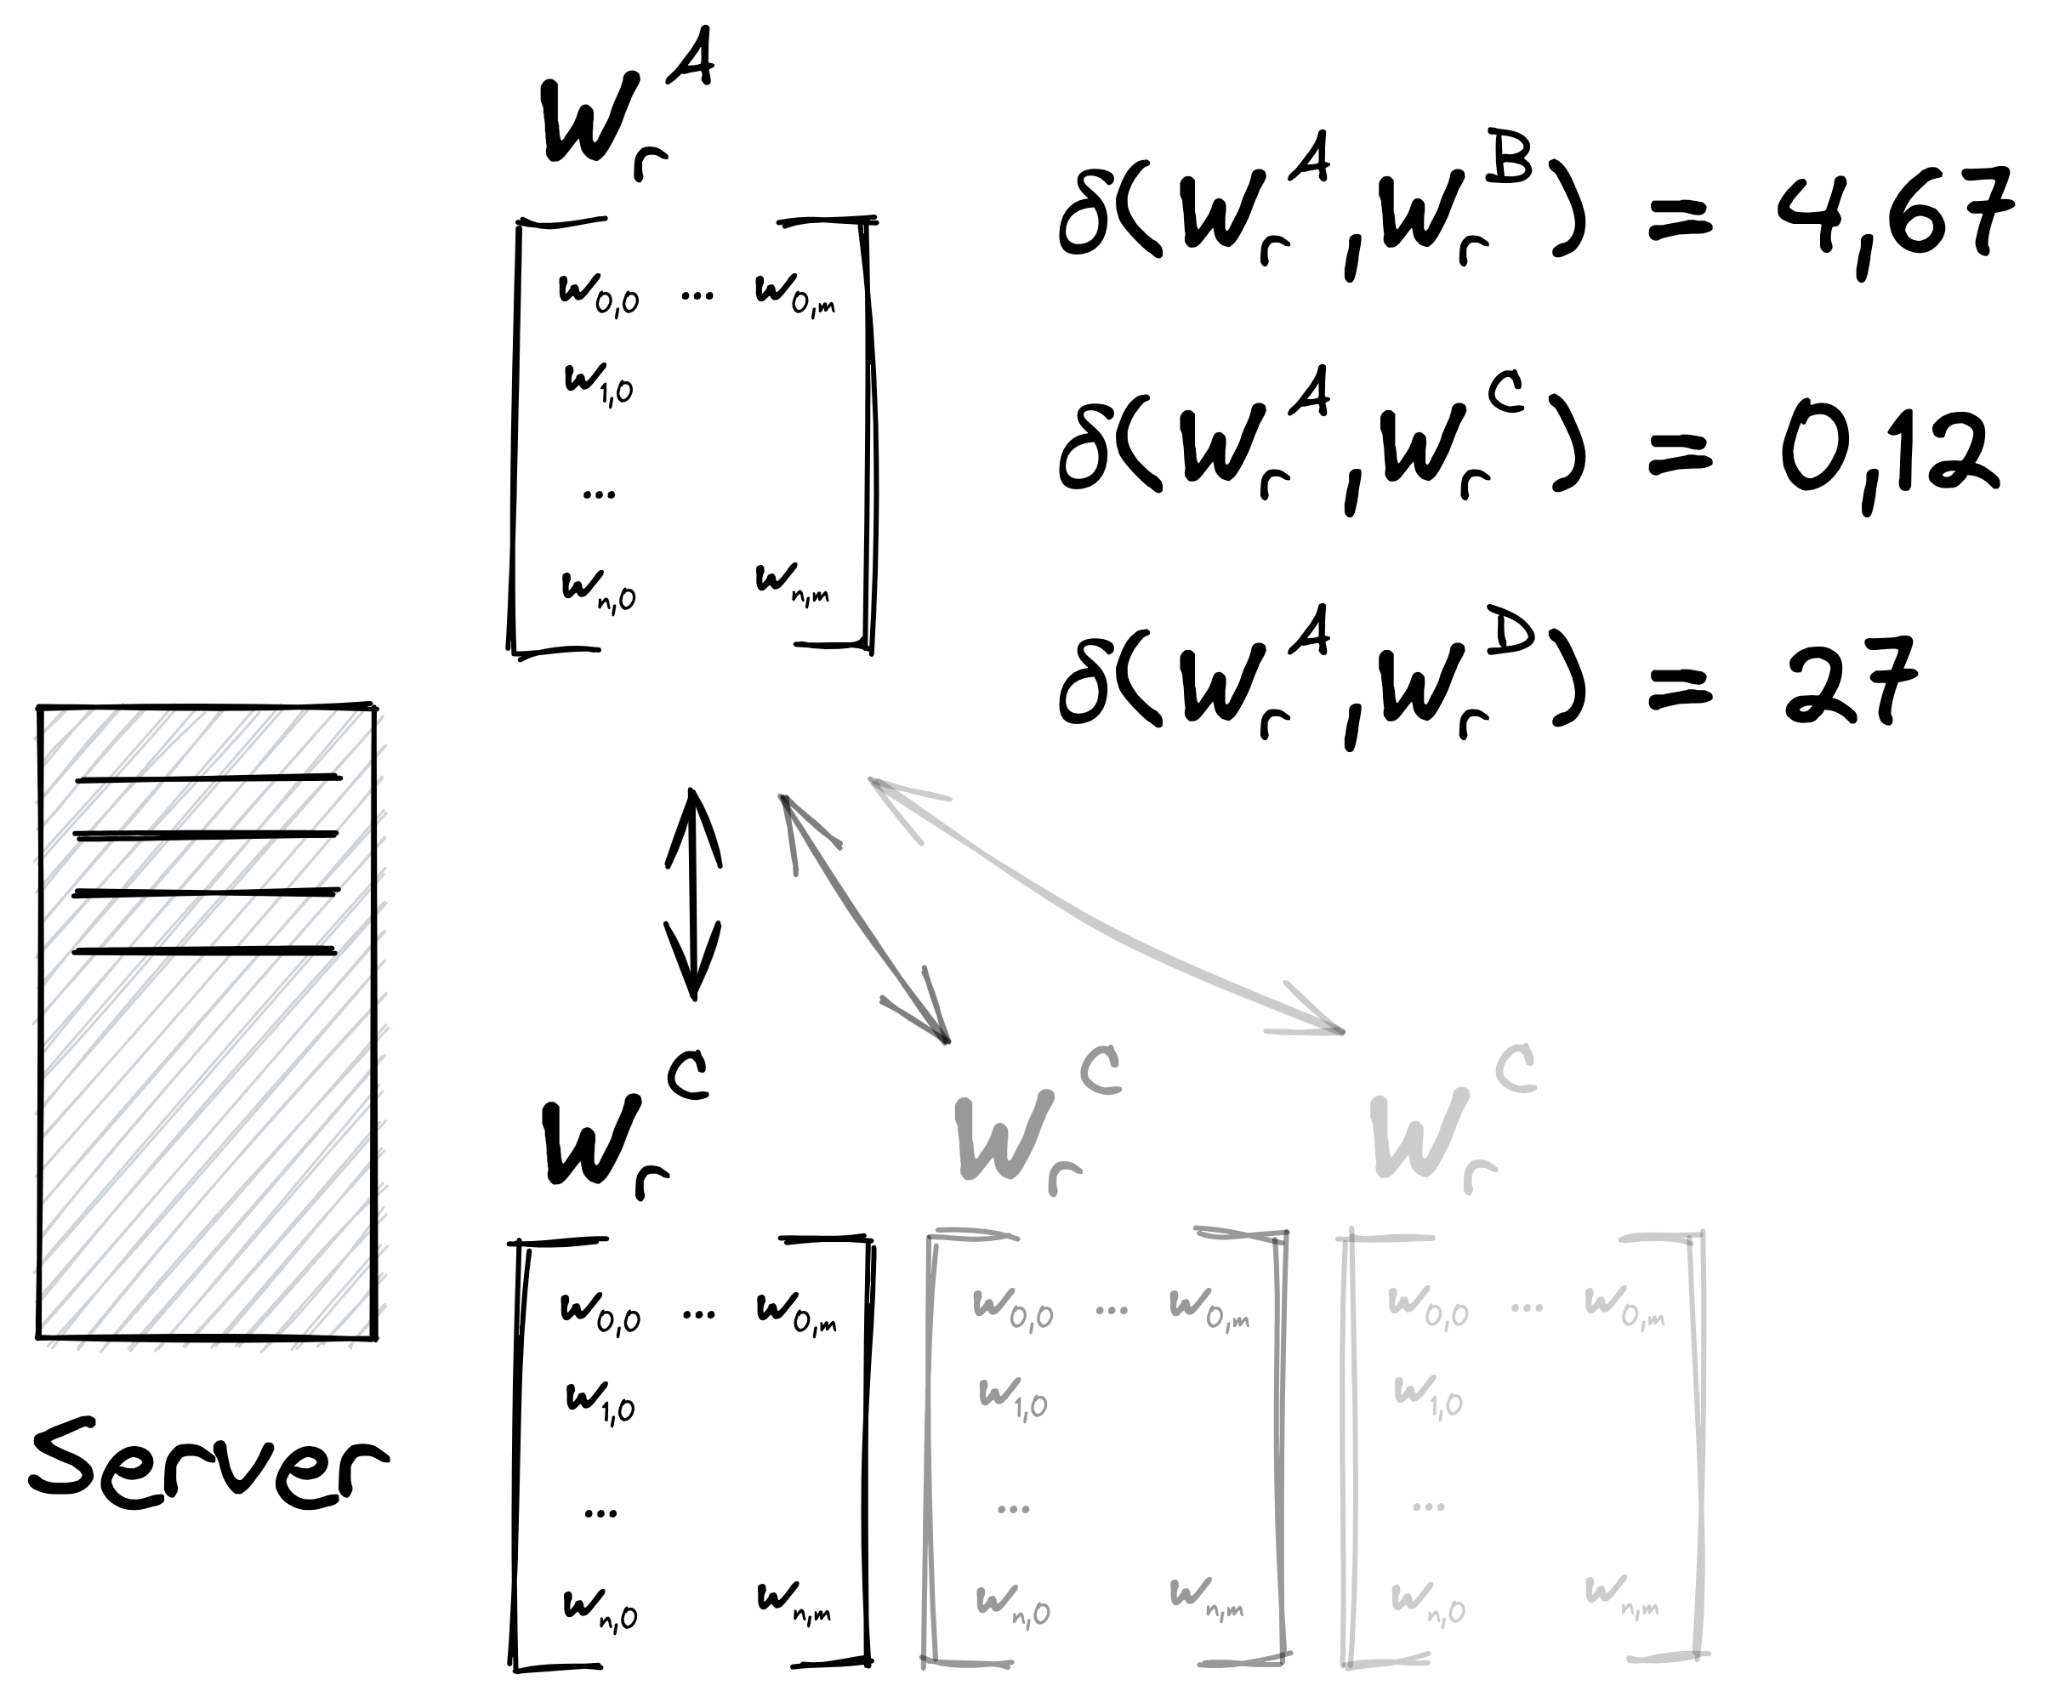
\includegraphics[height=.36\textheight]{figures/thesis/radar/server-side-comp}
%         \end{figure}

%         \begin{itemize}\footnotesize
%           \item Less related to client data.
%         \end{itemize}
%       \end{column}%
%     }

%     \onslide<3->{%
%       \begin{column}{.33\textwidth}
%         \footnotesize\centering
%         \textbf{Client-side evaluation}~\autocite{zhao_ShieldingCollaborativeLearning_2020}

%         \begin{figure}
%           \centering
%           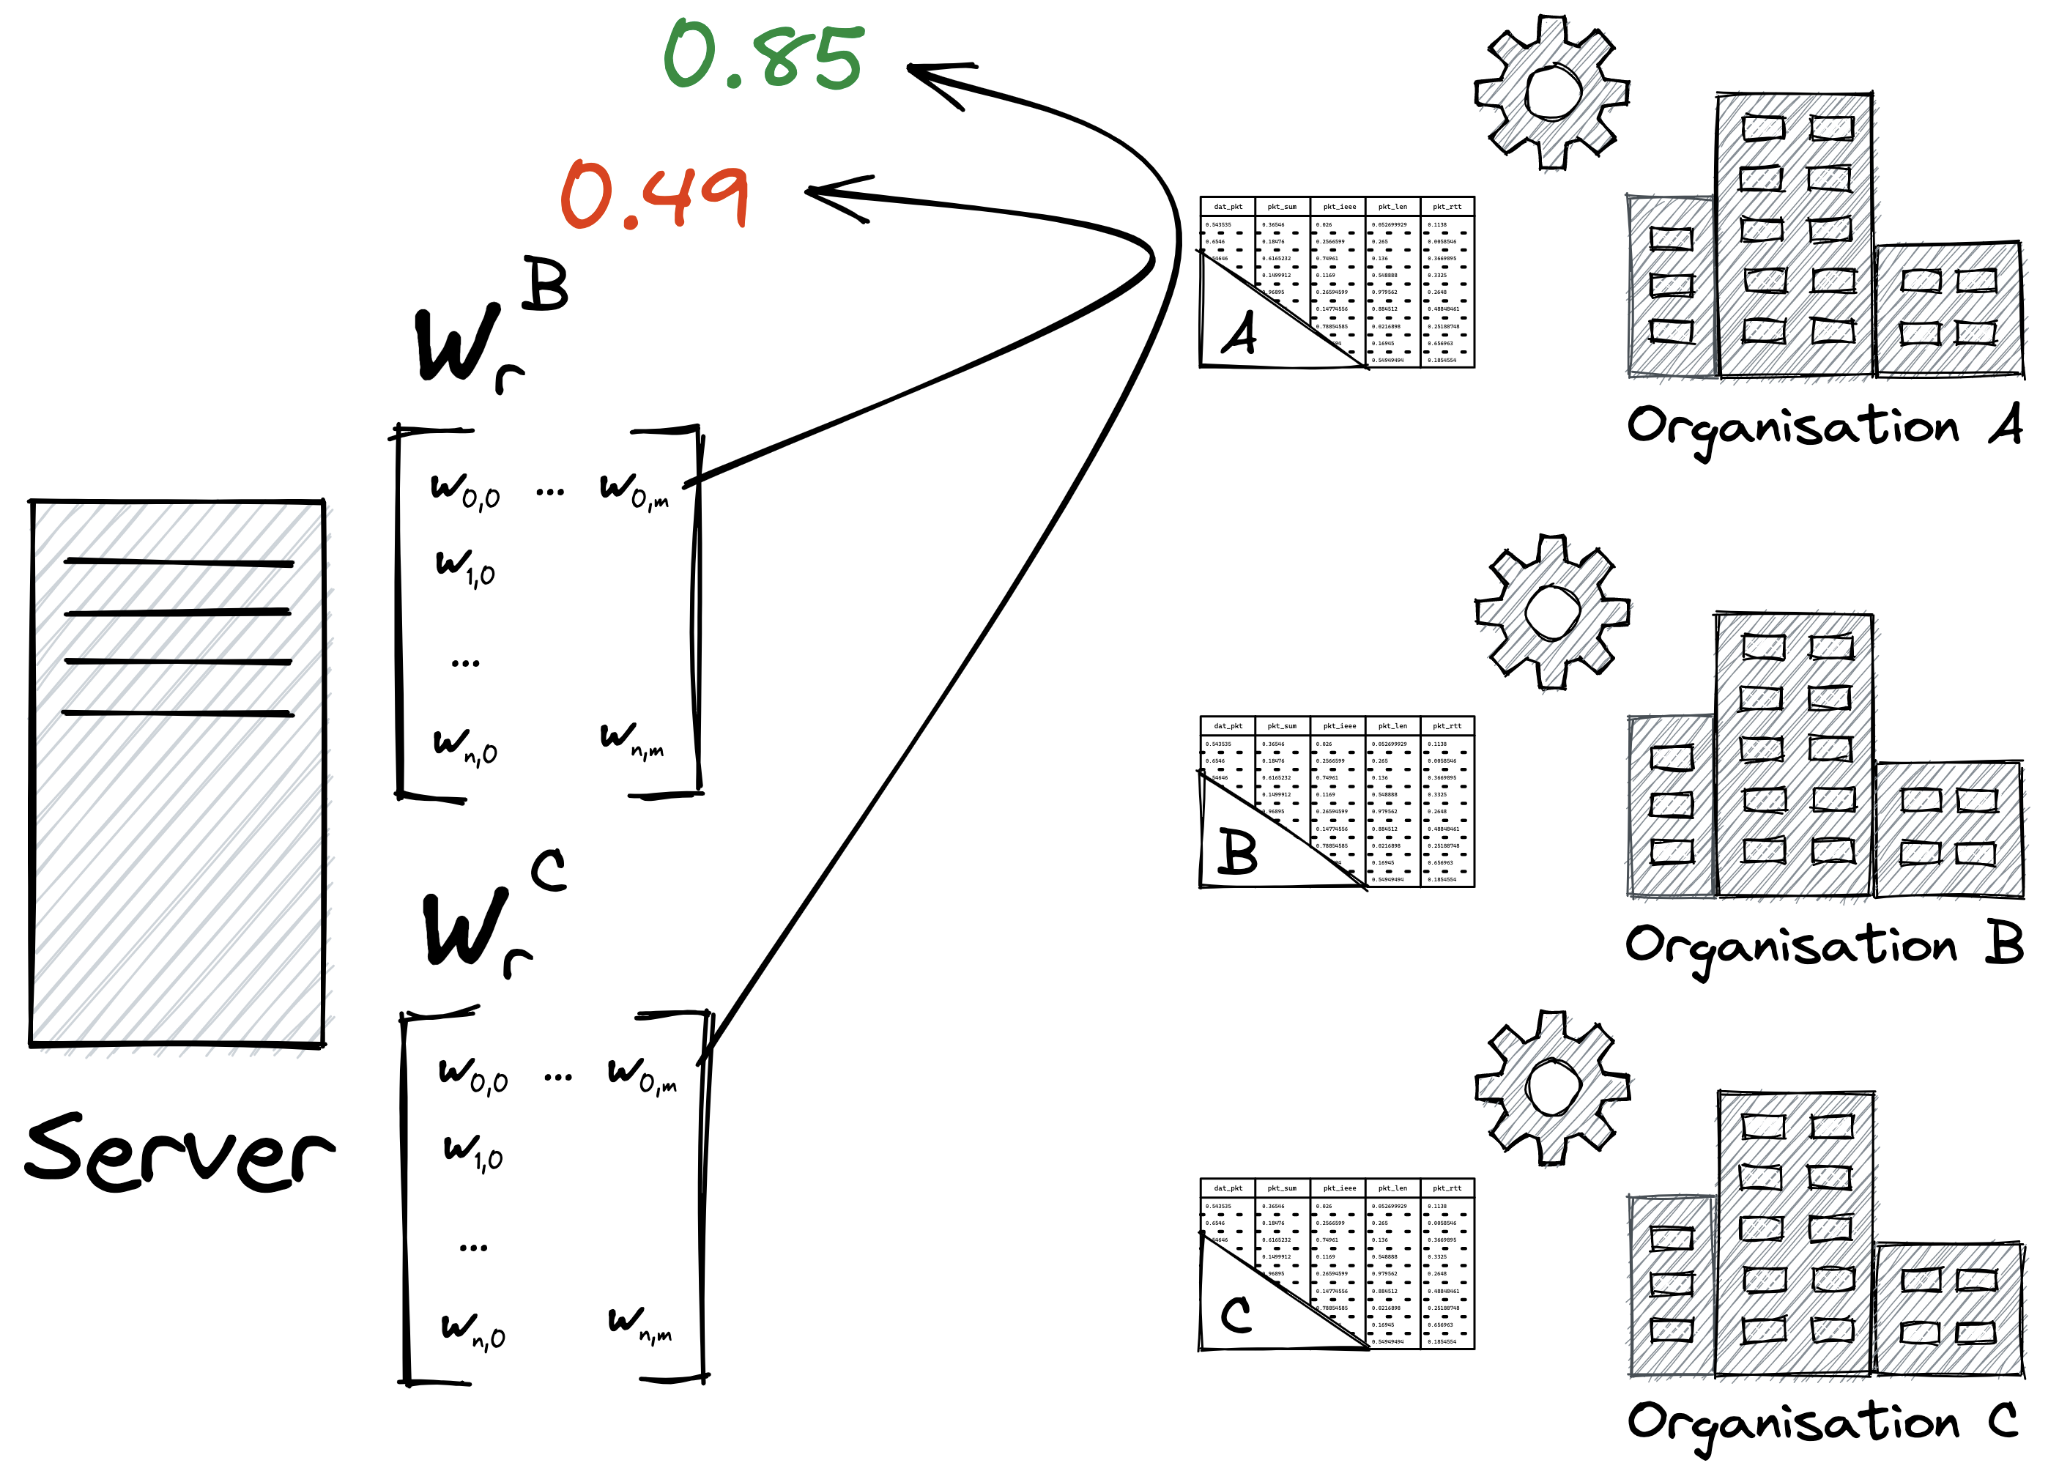
\includegraphics[height=.36\textheight]{figures/thesis/radar/client-side-eval}
%         \end{figure}

%         \begin{itemize}\footnotesize
%           \item High cost in cross-device.
%           \item More susceptible to badmouthing.
%         \end{itemize}
%       \end{column}%
%     }

%   \end{columns}

%   \vspace{3ex}
  
%   \footcite*{zhou_DifferentiallyPrivateFederated_2022}
%   \only<1>{\blankfootnote{}\blankfootnote{}\blankfootnote{}} % To keep the same height for the footnotes.
%   \only<2->{\footcite*{briggs_Federatedlearninghierarchical_2020}}
%   \only<2>{\blankfootnote{}}
%   \only<3->{\footcite*{zhao_ShieldingCollaborativeLearning_2020}}

% \end{frame}
% \endgroup

\begin{frame}{Introducing \texttt{RADAR}}
  \centering
    \begin{figure}
      \centering
      \foreach \i in {1,...,4} {
        \includegraphics<\i>[width=.95\linewidth,left]{figures/thesis/radar/agenda/\i.pdf}%
      }
      \vspace{-2em}
      \caption{\texttt{RADAR}~\footcite{lavaur_radar_2024} architecture, combining \emph{subjective} clustering and reputation-weighted aggregation to mitigate the impact lower-quality contributions.}
      \label{fig:radar}
    \end{figure}  
\end{frame}

% \begin{frame}{Assessing Quality with Cross-Evaluation}

%   \begin{columns}
%     \begin{column}{.45\textwidth}
%       \begin{figure}
%         \centering
%         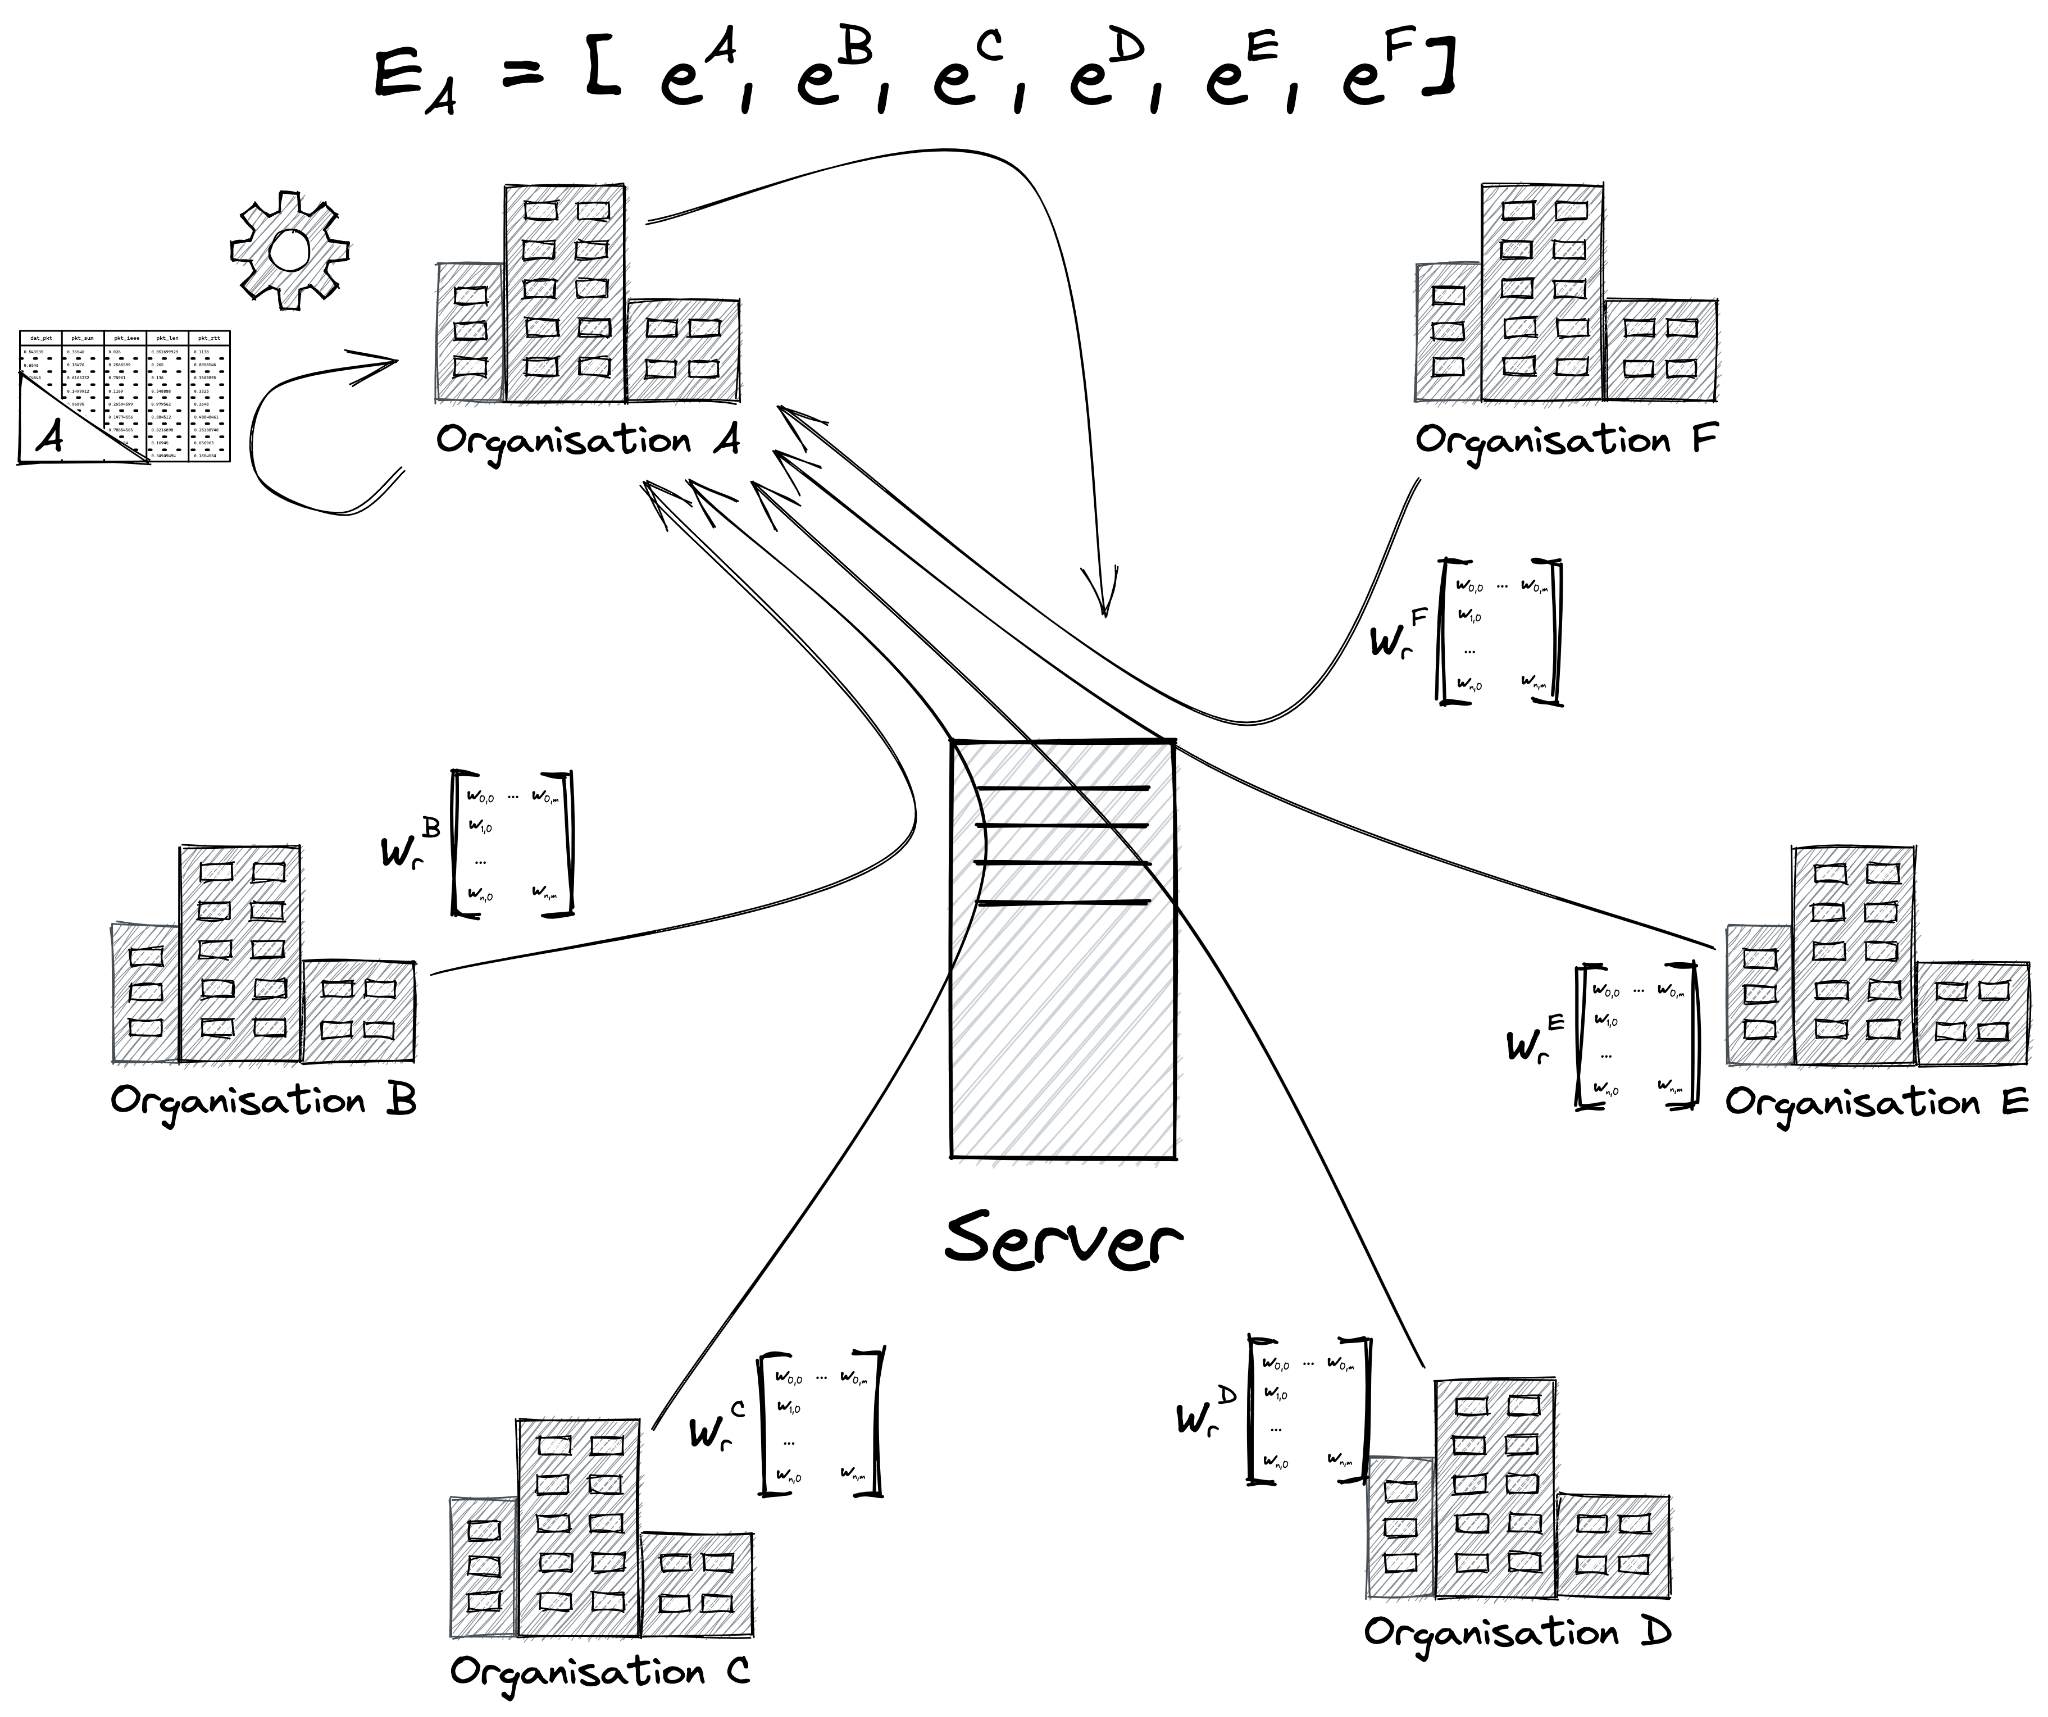
\includegraphics[width=\textwidth]{figures/thesis/radar/xeval}
%       \end{figure}
%     \end{column}
    
%     \begin{column}{.55\textwidth}
%       \footnotesize
%       \setlength{\baselineskip}{0.8\baselineskip}
%       \vspace{1ex}

%       \textbf{Advantages}
%       \begin{itemize}
%         \item Exhaustive overview of the entire system at each round $r$. \alert{No prior knowledge!}
%         \item Evaluations (\eg, accuracy, F1 score) representative of participants' data.
%       \end{itemize}
%       \medskip
%       \pause
%       \textbf{Drawbacks}
%       \begin{itemize}
%         \item High communication and computation costs.
%         \item Does not scale well.
%       \end{itemize}
%       \medskip
%       \pause
%       \textbf{But\dots}
%       \begin{itemize}
%         \item Cross-silo use case: few clients, with reasonable computing capacity.
%         \item Slow workflow: long time between rounds.
%       \end{itemize}
%     \end{column}

%   \end{columns}

% \end{frame}



% \begin{frame}{Fighting Heterogeneity with Clustering}
%   \bigskip\bigskip
%   \centering
%   \begin{minipage}{.8\textwidth}
%     \textbf{Objective}
%     \begin{itemize}
%       \item Build \emph{more} homogeneous communities of participants to facilitate model aggregation.
%     \end{itemize}    
%   \end{minipage}

  
%   \begin{columns}
%     \begin{column}{.5\textwidth}
%       \pause
%       \begin{itemize}
%         \item Distance metric
%         \begin{itemize}
%             \item Based on \alert{cross-evaluation} results. 
%             \item \alert{Cosine similarity}~\autocite{briggs_Federatedlearninghierarchical_2020}.
%         \end{itemize}
%       \end{itemize}
      
%       \pause
%       \begin{itemize}
%         \item Algorithm
%         \begin{itemize}
%           \item \alert{Hierarchical clustering}.~\autocite{briggs_Federatedlearninghierarchical_2020}
%           \item Dynamic aggregation threshold. 
%         \end{itemize}
%       \end{itemize}
%     \end{column}


%       \begin{column}{.5\textwidth}
%         \begin{figure}
%           \centering
%           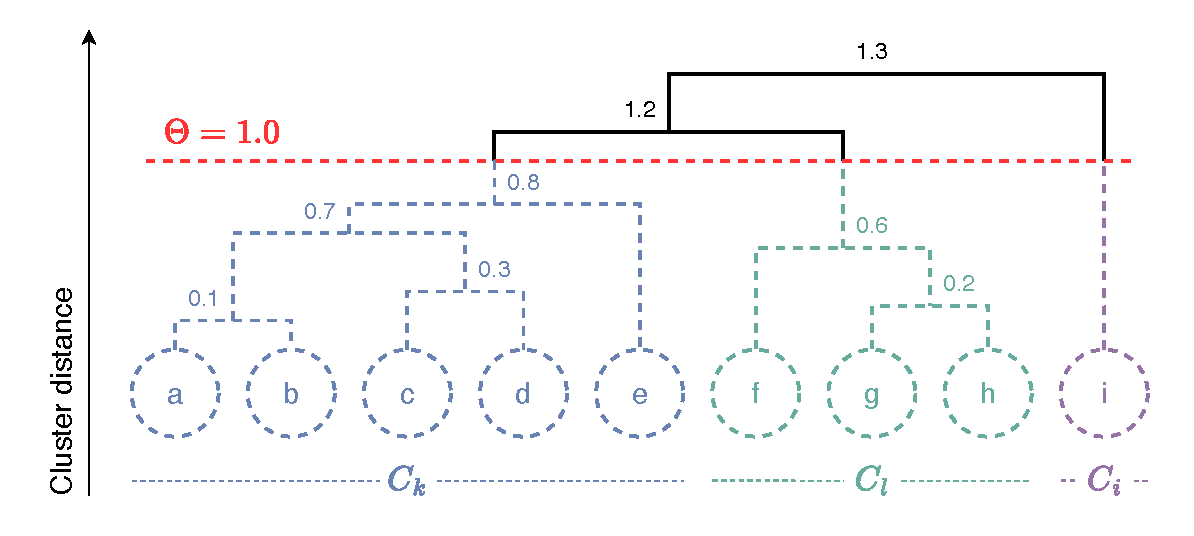
\includegraphics[width=\textwidth]{figures/thesis/radar/clustering.drawio.pdf}
%           \caption{Hierarchical clustering.}
%         \end{figure}
%       \end{column}
%   \end{columns}
%   \bigskip
%   \only<2->{\footcite*{briggs_Federatedlearninghierarchical_2020}}

% \end{frame}

% \begin{frame}{Reputation-aware Aggregation}
%   \begin{block}{Definition: Reputation Systems\normalfont~\autocite{resnick_Reputationsystems_2000}}
%     \begin{itemize}
%       \item Long-lived entities expecting future interaction.
%       \item Capture and distribution of feedback about current interactions (such information must be visible in the future).
%       \item Use of feedback to guide trust decisions.
%     \end{itemize}
%   \end{block}
%   \footcite*{resnick_Reputationsystems_2000}

%   % \pause
%   % \begin{itemize}
%   %   \item Votes weighted by the similarity inside each cluster.
%   %   \item Exponential decay for potential redemption.
%   % \end{itemize}

% \end{frame}

% \begin{frame}{Setup: Simulating Practical Heterogeneity}

%     \begin{columns}
%       \begin{column}{.4\textwidth}
%         \textbf{Datasets}
%         \begin{itemize}
%           \item Heterogeneous datasets, but some participants can share similarities.
%           \item 4 datasets: CIC-CSE-IDS2018, UNSW-NB15, Bot-IoT, ToN\_IoT.
%           \item NF-V2~\autocite{sarhan_StandardFeatureSet_2021} feature set (\ie, NetFlow V9).
%         \end{itemize}
%       \end{column}
%       \begin{column}{.56\textwidth}
%         \begin{figure}
%           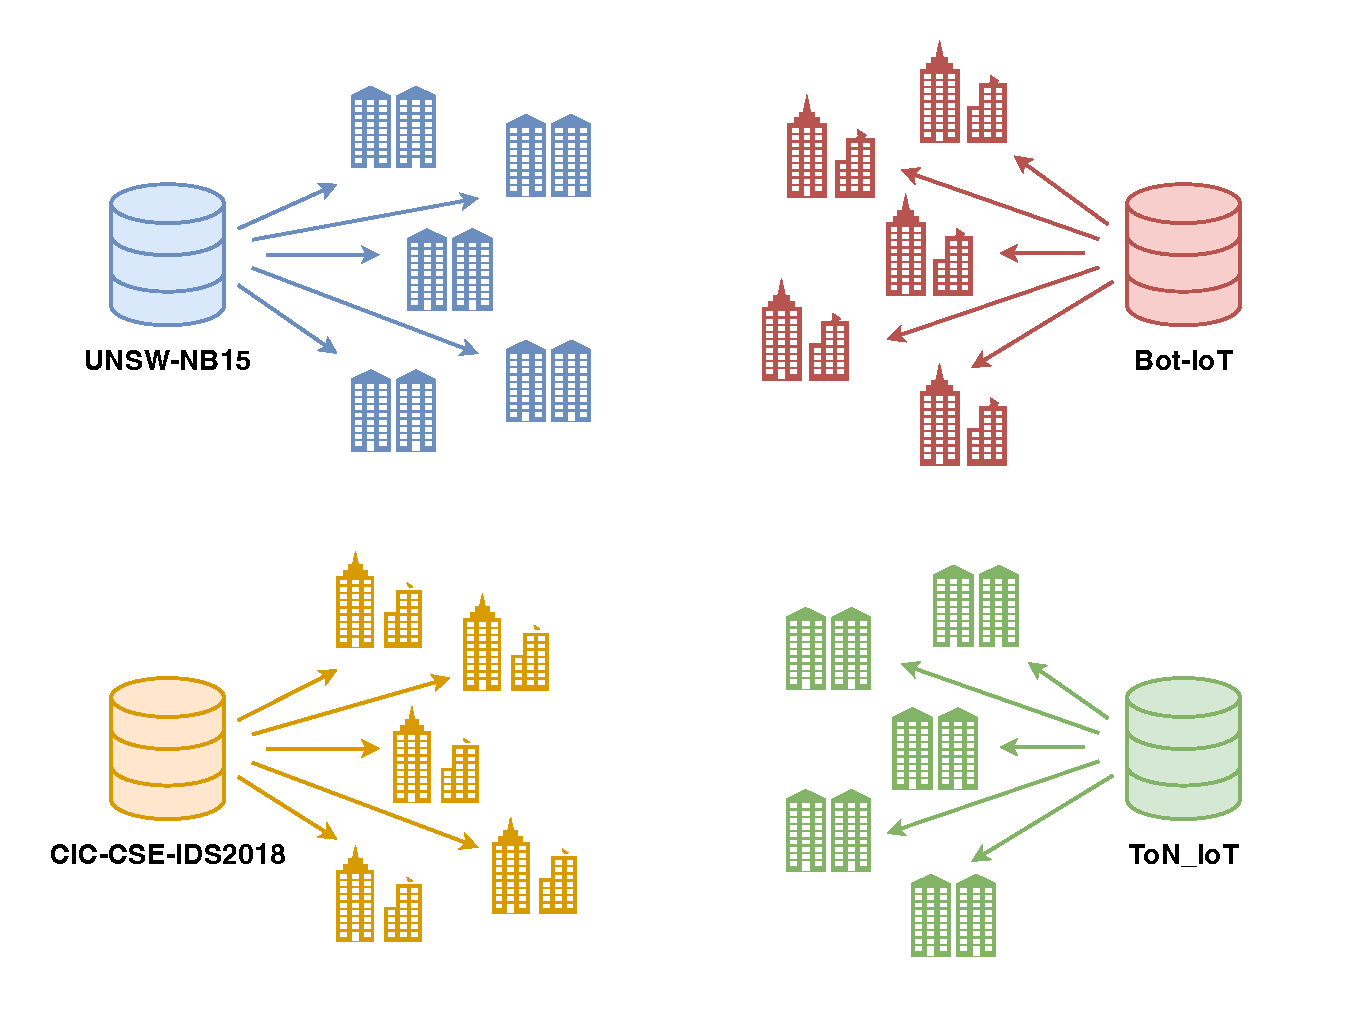
\includegraphics[width=\linewidth]{figures/thesis/radar/partition.pdf}%
%         \end{figure}
%       \end{column}
%     \end{columns}
%     \footcite*{sarhan_StandardFeatureSet_2021}
%   \end{frame}
  
  % \begin{frame}{Setup: Byzantine Scenarios}
  %     \begin{columns}
  %         \begin{column}{.4\textwidth}
  %             \textbf{Parameters}
  %             \begin{itemize}
  %                 \item \textit{Target}: Affected classes.
  %                 \item \textit{Data Poisoning Rate (DPR)}: proportion of targeted data with flipped labels.
  %                 \item \textit{Model Poisoning Rate (MPR)}: number of attackers in the cluster.
  %             \end{itemize}
  %         \end{column}
  %         \begin{column}{.56\textwidth}
  %           \begin{figure}
  %             \captionsetup{font=small, labelfont=small}
  %             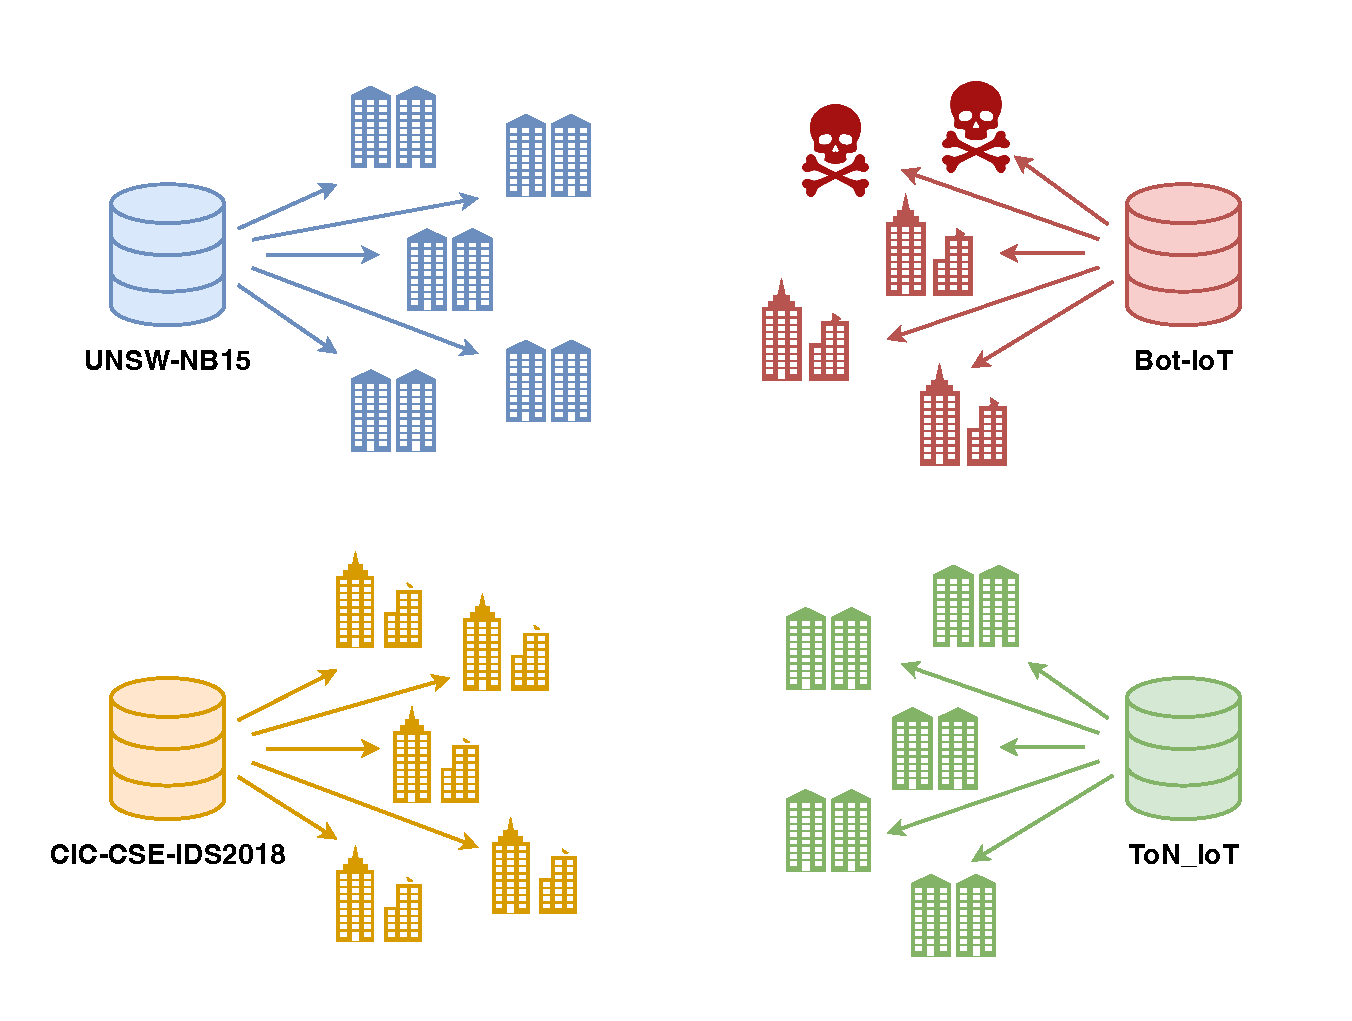
\includegraphics[width=\linewidth]{figures/thesis/radar/poisoning.pdf}%
  %             \captionsetup{justification=centering}
  %             \caption*{
  %               \texttt{colluding minority 100T}\\
  %               \footnotesize (\ie, 2 attackers, 100\% DPR on Reconnaissance class).
  %             }
  %           \end{figure}
  %         \end{column}
  %     \end{columns}
  % \end{frame}

% \begin{frame}{Results}
%   \begin{columns}
%     \column{.5\textwidth}
%     \begin{figure}
%       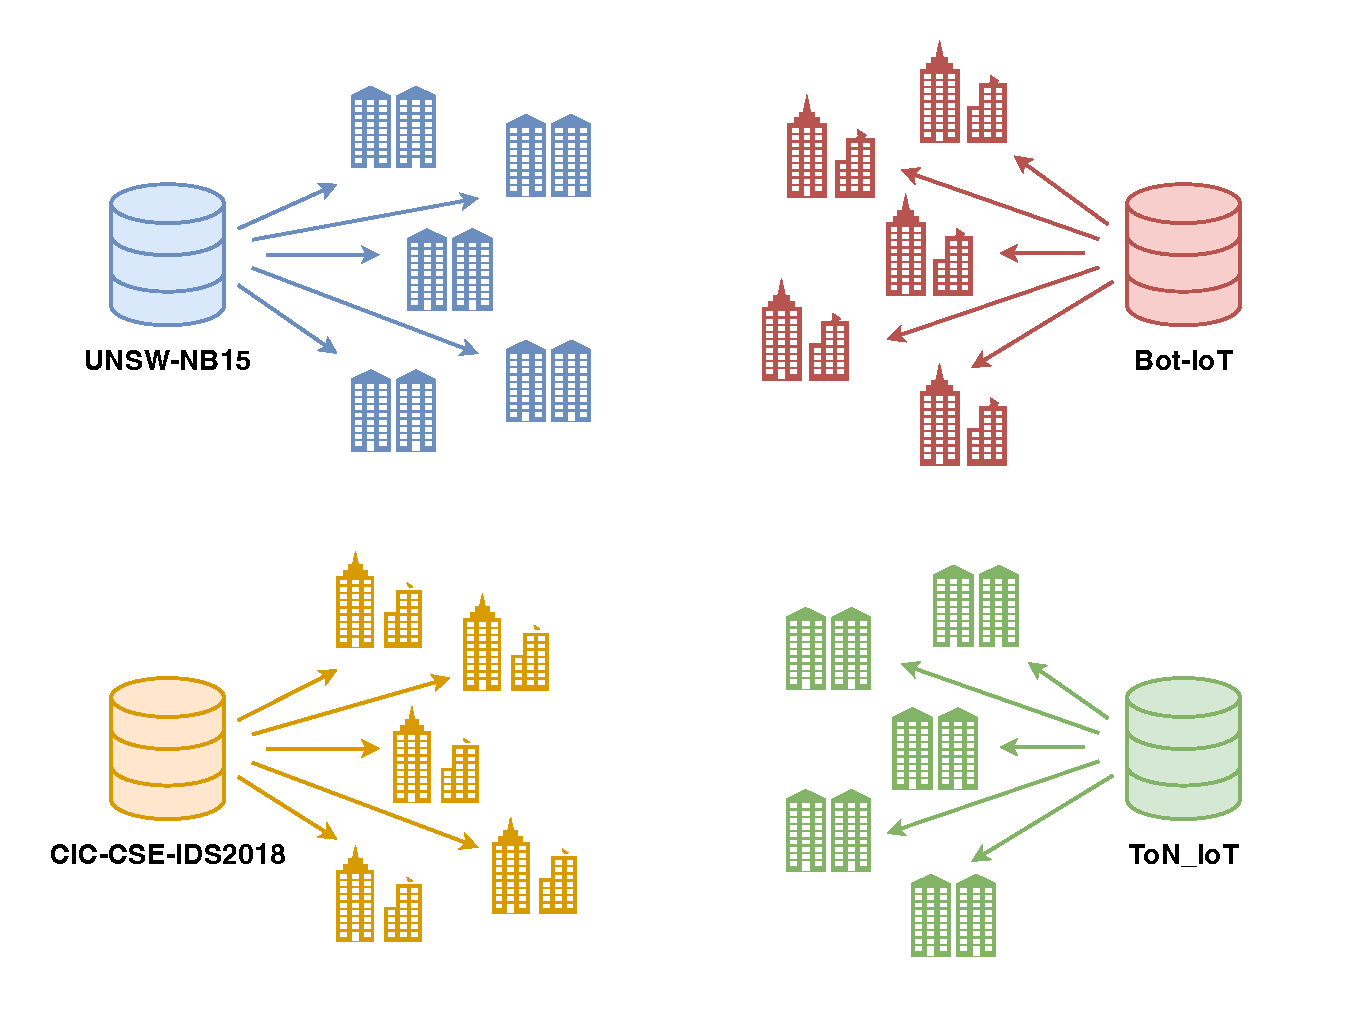
\includegraphics[width=.9\linewidth]{figures/thesis/radar/partition.pdf}%
%       \caption{Emulating heterogeneity using unified feature set on multiple datasets.}
%     \end{figure}

%     \column{.5\textwidth}
%     \renewcommand{\hl}{\cellcolor{white}}
%     \only<2>{\renewcommand{\hl}{\cellcolor{green!30}}}
%     \begin{table}
%       \centering
%       \caption{
%         \textit{Effect of different attack configurations (untargeted) on all baselines.}
%         \texttt{RA} is RADAR, \texttt{FG} is \texttt{FoolsGold}, \texttt{FA} is \texttt{FedAvg} (on \textit{all} participants), and \texttt{FC} is \texttt{FedAvg} ideally clustered per dataset.
%       }
%       \footnotesize
%       \setlength\tabcolsep{1ex}
%       \begin{tabularx}{\textwidth}{l>{\raggedright\arraybackslash}p{2.15cm}|rrrr}
%         \toprule % ---------------------------------
%         \multicolumn{2}{c|}{\multirow{2}{*}{\textbf{Scenario}}} & \multicolumn{4}{c}{\textbf{\gls{asr}} (\%, \textit{lower is better})} \\
%         & & \multicolumn{1}{c}{\texttt{RA}} & \multicolumn{1}{c}{\texttt{FG}} & \multicolumn{1}{c}{\texttt{FA}} & \multicolumn{1}{c}{\texttt{FC}} \\
%         \midrule % ---------------------------------
%         % TARGETED ATTACKS
%         \multicolumn{2}{l|}{\textbf{Targeted} (\texttt{100T})} & & & & \\
%           & \hl \texttt{Benign}       &  \hl \textbf{0.00} &  5.17 & 5.10 &  0.09 \\
%           & \hl \texttt{Lone}         &  \hl \textbf{0.00} & 93.82 & 6.73 &  0.45 \\
%           & \hl \texttt{Collud.~min.} &  \hl \textbf{0.00} &  2.97 & 9.99 & 53.40 \\
%           & \only<3>{\cellcolor{red!20}} \texttt{Collud.~maj.} &  \only<3>{\cellcolor{red!20}} 73.39 & \textbf{8.10} & 17.65 & 59.36 \\
%         \midrule % ---------------------------------
%         % UNTARGETED ATTACKS
%         \multicolumn{2}{l|}{\textbf{Untargeted} (\texttt{100U})} & & & & \\
%         & \hl \texttt{Benign}        & \hl 0.09  & 0.39 & 33.30 & \textbf{0.06} \\
%         & \hl \texttt{Lone}          & \hl \textbf{0.08} & 99.89 & 54.70 & 0.12 \\
%         & \hl \texttt{Collud.~min.}  & \hl 0.10 & \textbf{0.04} & 44.53 & 6.26 \\
%         & \hl \texttt{Collud.~maj.}  & \hl \textbf{0.08} & 38.98 & 59.49 & 94.36 \\
%         \bottomrule% ---------------------------------
%       \end{tabularx}
%     \end{table}
%   \end{columns}
% \end{frame}

\newcommand{\hr}{\cellcolor{red!30}}
\newcommand{\ho}{\cellcolor{orange!30}}
\newcommand{\hg}{\cellcolor{green!30}} 

\begin{frame}{Handling heterogeneity}
  \begin{columns}
    \begin{column}{.4\textwidth}
      \begin{figure}
              \captionsetup{justification=centering}
        \includegraphics<1>[width=\linewidth,left]{./figures/radar-eval/clustering/clustering_benign.pdf}%
        \caption{Clustering results without poisoning.\\ 
        Rand index=1.0}
      \end{figure}
    \end{column}
  \begin{column}{.6\textwidth}

\begin{table}
    \centering
    \caption*{Accuracy for different baselines.}
    \footnotesize
    \setlength\tabcolsep{1ex}
    \begin{tabularx}{.7\textwidth}{>{\raggedright\arraybackslash}p{2.15cm}|ccc}
      \toprule % ---------------------------------
      \textbf{Scenario}
      & \multicolumn{1}{c}{\texttt{RADAR}} & \multicolumn{1}{c}{\texttt{FoolsGold}} & \multicolumn{1}{c}{\texttt{Clustered}} \\
      \midrule % ---------------------------------
      \textbf{Benign} & \hg 99.07 & \hr 55.04 & \hg 99.24  \\
    \end{tabularx}
    \caption*{\footnotesize More is better}

  \end{table}
    \end{column}
  \end{columns}
\end{frame}

%%%%%%%%%%%%
%Untargeted
%%%%%%%%%%%%
\begin{frame}{Handling Untargeted Byzantines}
  \begin{columns}
    \begin{column}{.4\textwidth}
      \begin{figure}
        \captionsetup{justification=centering}
        \only<1>{
            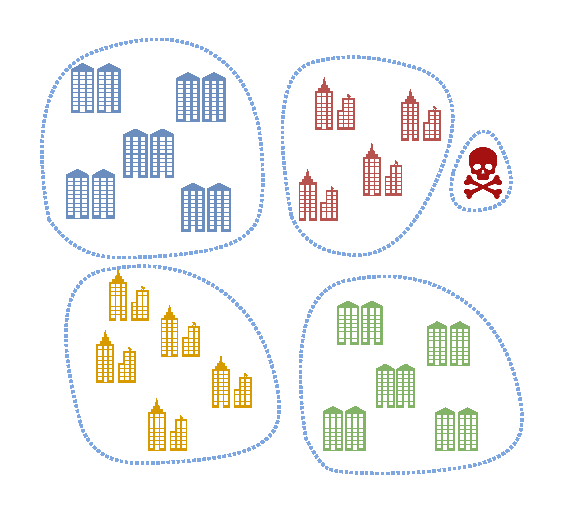
\includegraphics[width=\linewidth,left]{./figures/radar-eval/clustering/clustering_lone_untargeted.pdf}
            \caption*{Clustering results for\\
            \texttt{lone 100U}.\\ 
            Rand index=1.0
            }
        }
        \only<2>{
            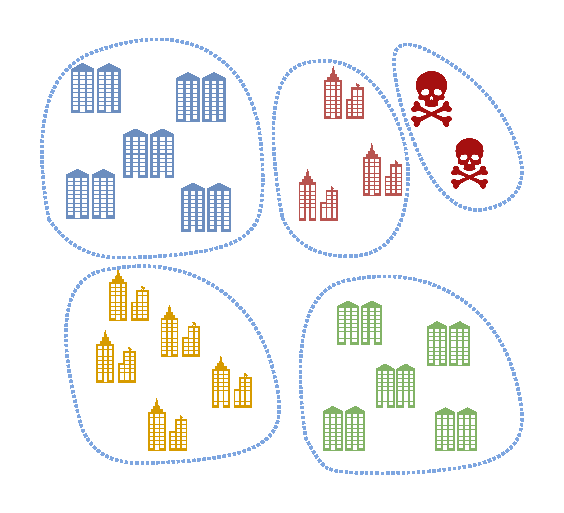
\includegraphics[width=\linewidth,left]{./figures/radar-eval/clustering/clustering_min_untargeted.pdf}
            \caption*{Clustering results for\\ \texttt{colluding minority 100U}\\ 
            Rand index=1.0
            }
        }
        \only<3>{
            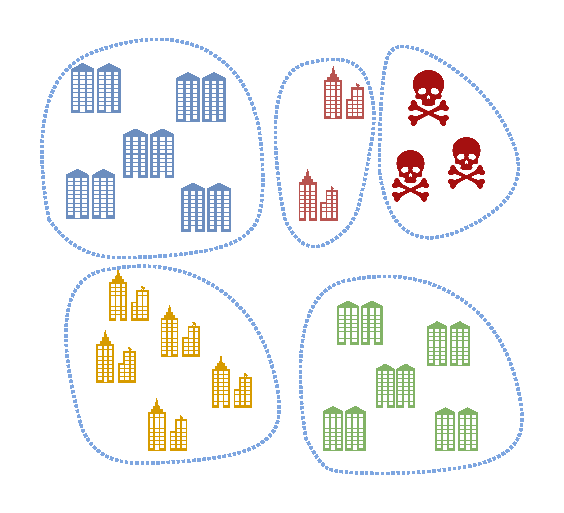
\includegraphics[width=\linewidth,left]{./figures/radar-eval/clustering/clustering_maj_untargeted.pdf}
          \caption*{Clustering results for\\
            \texttt{colluding majority 100U}\\ 
            Rand index=1.0
            }
        }        
      \end{figure}
    \end{column}

  \begin{column}{.6\textwidth}
    \begin{table}
        \centering
    
        \footnotesize
        \setlength\tabcolsep{1ex}
        \caption*{Attack success rate for different baselines.}  
        \begin{tabularx}{.8\textwidth}{l>{\raggedright\arraybackslash}p{2.15cm}ccc}
          \toprule % ---------------------------------
          \multicolumn{2}{c}{{\textbf{Scenario}}}
          & \multicolumn{1}{c}{\texttt{RADAR}} & \multicolumn{1}{c}{\texttt{FoolsGold}} & \multicolumn{1}{c}{\texttt{Clustered}} \\
          \midrule % ---------------------------------
          % % UNTARGETED ATTACKS
          \multicolumn{2}{l}{\textbf{Untargeted} (\texttt{100U})}  & & & \\
          & \texttt{Lone} & \hg 0.08 &\hr 99.89 & \hg 0.12 \\
          \only<2->{& \texttt{Collud. min.} & \hg 0.10 & \hg 0.04 &\ho 6.26 \\}
          \only<3->{& \texttt{Collud. maj.} & \hg 0.08 &\ho 38.98 & \hr 94.36 \\}
          \end{tabularx}
          \caption*{\footnotesize Less is better}
      \end{table}
  
     \end{column}
  \end{columns}
\end{frame}


%%%%%%%%%%%%    
% Targeted   
%%%%%%%%%%%%

\begin{frame}{Handling Targeted Byzantines}
    \begin{columns}
        \begin{column}{.4\textwidth}
            \begin{figure}
                \centering
                \captionsetup{justification=centering}
                \only<1-2>{%
                    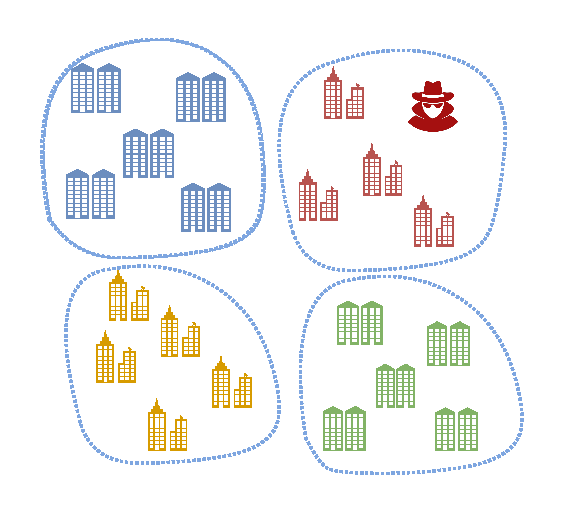
\includegraphics[width=\linewidth,left]{figures/radar-eval/clustering/clustering_lone_targeted.pdf}
                    \caption*{
                        Clustering results for\\
                        \texttt{Lone 100T}\\ 
                        Rand index=0.97
                    }
                }
                \only<3>{%
                    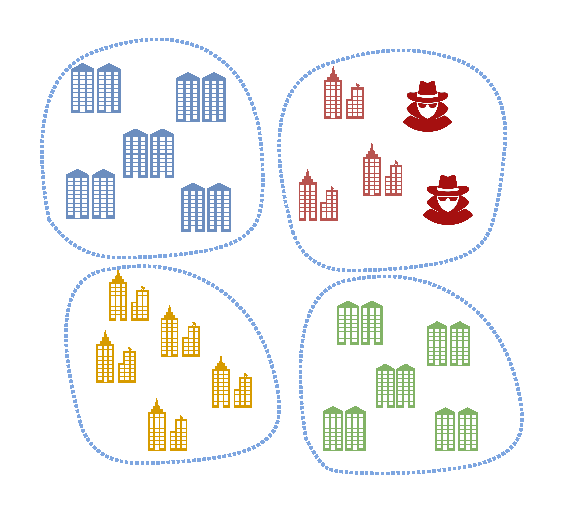
\includegraphics[width=\linewidth,left]{./figures/radar-eval/clustering/clustering_min_targeted.pdf}%
                    \caption*{
                        Clustering results for\\
                        \texttt{colluding minority 100T}\\ 
                        Rand index=0.97
                    }
                }
                \only<4>{
                    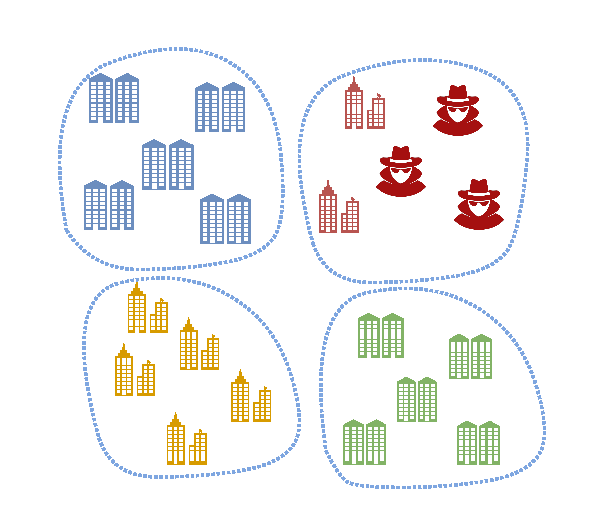
\includegraphics[width=\linewidth,left]{./figures/radar-eval/clustering/clustering_maj_targeted.pdf}%
                    \caption*{Clustering results for \texttt{colluding majority 100T}\\ 
                    Rand index=0.96}
                }
                
            \end{figure}
        \end{column}
        \begin{column}{.6\textwidth}
            \begin{table}
                \centering
                \footnotesize
                \setlength\tabcolsep{1ex}
                \caption*{Attack success rate for different baselines.}  

                \begin{tabularx}{.8\textwidth}{l>{\raggedright\arraybackslash}p{2.15cm}ccc}
                    \toprule % ---------------------------------
                    \multicolumn{2}{c}{{\textbf{Scenario}}}
                    & \multicolumn{1}{c}{\texttt{RADAR}} & \multicolumn{1}{c}{\texttt{FoolsGold}} & \multicolumn{1}{c}{\texttt{Clustered}} \\
                    \midrule % ---------------------------------
                    % % TARGETED ATTACKS
                    \multicolumn{2}{l}{\textbf{Targeted} (\texttt{100T})}  & & & \\    
                    & \texttt{Lone} &\hg 0.00 & \hr 93.82 & \hg 0.45 \\
                    \only<3->{& \texttt{Collud. min.} & \hg 0.00 & \hg 2.97 & \hr 53.40 \\}
                    \only<4->{& \texttt{Collud. maj.} &  \hr 73.39 & \ho 8.10 & \hr 59.36 \\}
                \end{tabularx}
                
                \caption*{\footnotesize Less is better}
            \end{table}
            \vspace{-1em}
            
            \only<2>{\begin{minipage}{\textwidth}
                \begin{figure}
                    \captionsetup{justification=centering}
                    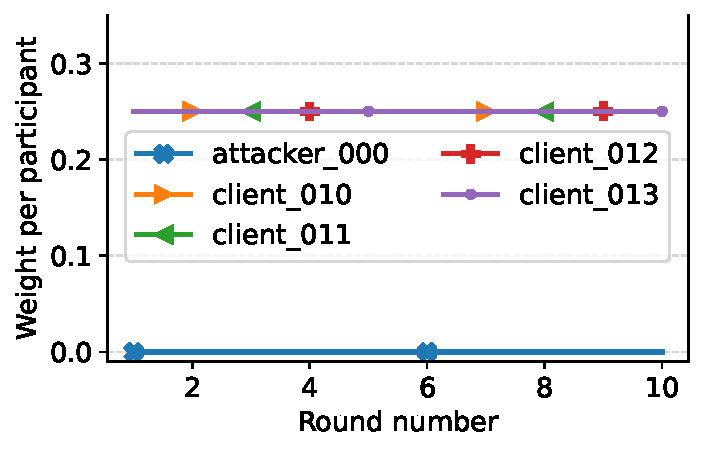
\includegraphics[width=.6\linewidth]{./figures/radar-eval/reput/lone_loud_expanded.pdf}
                    \caption{Aggregation weights.}
                \end{figure}
            \end{minipage}}

          %   \only<5>{\begin{minipage}{\textwidth}
          %       \begin{figure}
          %           \captionsetup{justification=centering}
          %           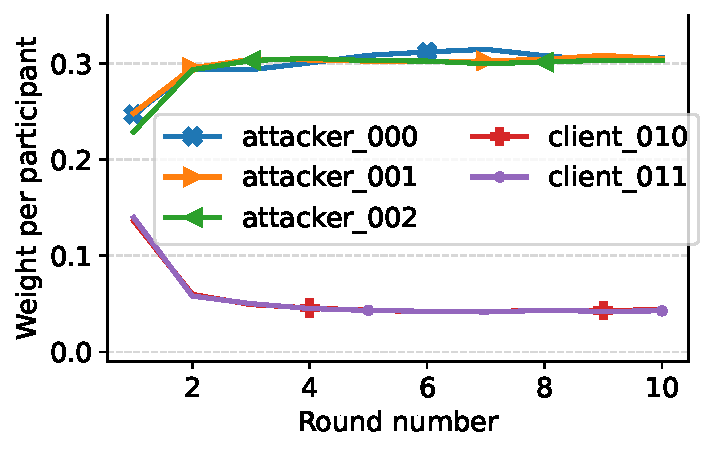
\includegraphics[width=.6\linewidth]{./figures/radar-eval/reput/byzantine_majority_loud_expanded.pdf}
          %           \caption{Aggregation weights.}
          %       \end{figure}
          %  \end{minipage}}

        \end{column}
    \end{columns}
\end{frame}



\begin{frame}{Highlights}
  % \begin{block}{Combining clustering and mitigation strategy is effective}
  %   Clustering effectively creates \alert{homogeneous} communities where conventional mitigation can be applied.
  % \end{block}

  % \pause
  \begin{block}{Cross-evaluation enable \alert{true} reputation-aware FL}
    Only way to gather indirect feedbacks (\ie, one clients' evaluation of another's contribution); at the cost of scalability.
  \end{block}

  \pause
  \begin{block}{Generalizable outside intrusion detection}
    With a few conditions: parametric models, locally owned evaluation set, a \alert{small-scale use case}, and a \alert{trusted central server}.
  \end{block}
\end{frame}

% \begin{frame}{Takeways}
%   \begin{enumerate}
%     \onslide<+->
%     \item \texttt{RADAR} can:
%     \begin{itemize}
%       \item leverage \alert{cross-evaluation}, \alert{clustering} and \alert{reputation} to address heterogeneity and Byzantine contributions;
%       \item adjust rapidly to changes in behavior; and
%       \item mitigate most tested scenarios (limiting case handled up to 80\% of poisoned data).
%     \end{itemize}

%     \medskip
%     \onslide<+->
%     \item How generic?
%     \begin{itemize}
%       \item Only few conditions: parametric models, locally owned evaluation set, a \alert<+->{small-scale use case}, and a \alert<.->{trusted central server}.
%     \end{itemize}

%     \medskip
%     \onslide<+->
%     \item Future works:
%     \begin{itemize}
%       \item Remove the central server dependency for \alert{increased trust and scalability}.
%       \item Test the approach in more realistic heterogeneous settings.
%     \end{itemize}
%   \end{enumerate}

% \end{frame}
% \subsection{\texorpdfstring{\feditn Generating Independent Datasets}{Generating Independent Datasets}}

\begin{frame}[plain]
  \subsectionpage
  
  \footcite*{lavaur_anubis_2025}
\end{frame}

{
  \setbeamertemplate{background}{
    \begin{tikzpicture}[remember picture,overlay]
      \node at (current page.south east)[anchor=south east,inner sep=0] {
\includegraphics[width=.6\paperwidth]{assets/backgrounds/background-white}};
    \end{tikzpicture}
  }
  \begin{frame}[plain]
    \centering
    \huge\itshape
    What datasets for \alert{distributed} intrusion detection?\\[1em]
    \pause
    \normalfont
    None (:
  \end{frame}
}

\begin{frame}{Existing workarounds}
  \begin{columns}[t]
    \begin{column}{0.45\textwidth}
      \centering\large
      \alert{Partitioning datasets}~\autocite{campos_EvaluatingFederatedLearning_2022}
    \end{column}
    \begin{column}{0.1\textwidth}
      \centering
      \vs
    \end{column}
    \begin{column}{0.45\textwidth}
      \centering\large
      \alert{Homogenizing features}~\autocite{popoola_FederatedDeepLearning_2021}
    \end{column}
  \end{columns}
  \pause
  \begin{columns}[t]
    \begin{column}{0.45\textwidth}
      \begin{itemize}
        \item Risk of correlation across clients and unrealistic data points;
        \item Requires a deep understanding of the dataset;
        \item Limited by the diversity of the selected dataset.
      \end{itemize}
    \end{column}
    \begin{column}{0.1\textwidth}\end{column}
    \begin{column}{0.45\textwidth}
      \pause
      \begin{itemize}
        \item Limited by the number of available datasets;
        \item No control over the data distribution;
        \item Lack dedicated test set.
      \end{itemize}
    \end{column}
  \end{columns}

  \footcite*{campos_EvaluatingFederatedLearning_2022,popoola_FederatedDeepLearning_2021}

\end{frame}


\begin{frame}{Project definition}
  \begin{block}{Objective}
  Design a systematic approach to generate \alert<+>{deployable} network topologies, capable of producing \alert<+>{heterogeneous} and \alert<+>{independent} datasets for evaluating Federated Intrusion Detection Systems (FIDSs).
  \end{block}

  \pause
  \begin{block}{Requirements}
    \begin{itemize}[<+->]
      \item \alert{diversity} in topologies, attacks and devices to provide heterogeneity;
      \item approach \alert{realism} in terms of traffic and behaviors;
      \item \alert{controllable} data distribution across clients;
      \item data \alert{independence} amongst clients;
    \end{itemize}
  \end{block}
\end{frame}

\begin{frame}{Related work}
  \begin{columns}[t]

    \onslide<+->
    \begin{column}{.33\textwidth}
      \begin{block}{Protocol testing~\autocite{doar_BetterModelGenerating_1996,medina_BRITEApproachUniversal_2001}}
        \begin{itemize}
          \item Internet-like topologies, not applicable to enterprise networks;
          \item focus on structural properties or degree distributions (\eg, power-law).
        \end{itemize}
      \end{block}
    \end{column}

    \onslide<.(1)->
    \begin{column}{.33\textwidth}
      \begin{block}{Usecase or task focused}
        \begin{itemize}[<+->]
          \item Declarative topology generation (\eg, \texttt{TopoGen}~\autocite{laurito_TopoGenNetworkTopology_2017} for SDN);
          \item Layer-based composition for Industrial Control Networks (\eg, \texttt{GENIND}~\autocite{alrumaih_GENINDIndustrialNetwork_2023});
        \end{itemize}
      \end{block}
    \end{column}
    
    \onslide<.(1)->
    \begin{column}{.33\textwidth}
      \begin{block}{Cyber-ranges}
        \begin{itemize}[<+->]
          \item Declarative deployments of scenarios and topologies~\autocite{venkatesan_VulnerVANVulnerableNetwork_2019,yamin_ModelingExecutingCyber_2022};
          \item Vulnerable environment generation from attack graphs (\eg, \texttt{URSID}~\autocite{besson_URSIDAutomaticallyRefining_2024}).
        \end{itemize}
      \end{block}
    \end{column}
  \end{columns}

  \only<1>{\footcite*{doar_BetterModelGenerating_1996,medina_BRITEApproachUniversal_2001}}
  \only<2>{\footcite*{laurito_TopoGenNetworkTopology_2017}}
  \only<3>{\footcite*{alrumaih_GENINDIndustrialNetwork_2023}}
  \only<4>{\footcite*{venkatesan_VulnerVANVulnerableNetwork_2019,yamin_ModelingExecutingCyber_2022}}
  \only<5>{\footcite*{besson_URSIDAutomaticallyRefining_2024}}  

\end{frame}

\begin{frame}{FedITN Approach Overview}
  % attack scenarios -> constraints -> compatible subtopologies -> topology trees
  \centering
  \includegraphics<1>[width=.9\textwidth]{figures/feditn/approach/overview-1}%
  \includegraphics<2>[width=.9\textwidth]{figures/feditn/approach/overview-2}%
\end{frame}

\begin{frame}{Topology composition}
  \centering
  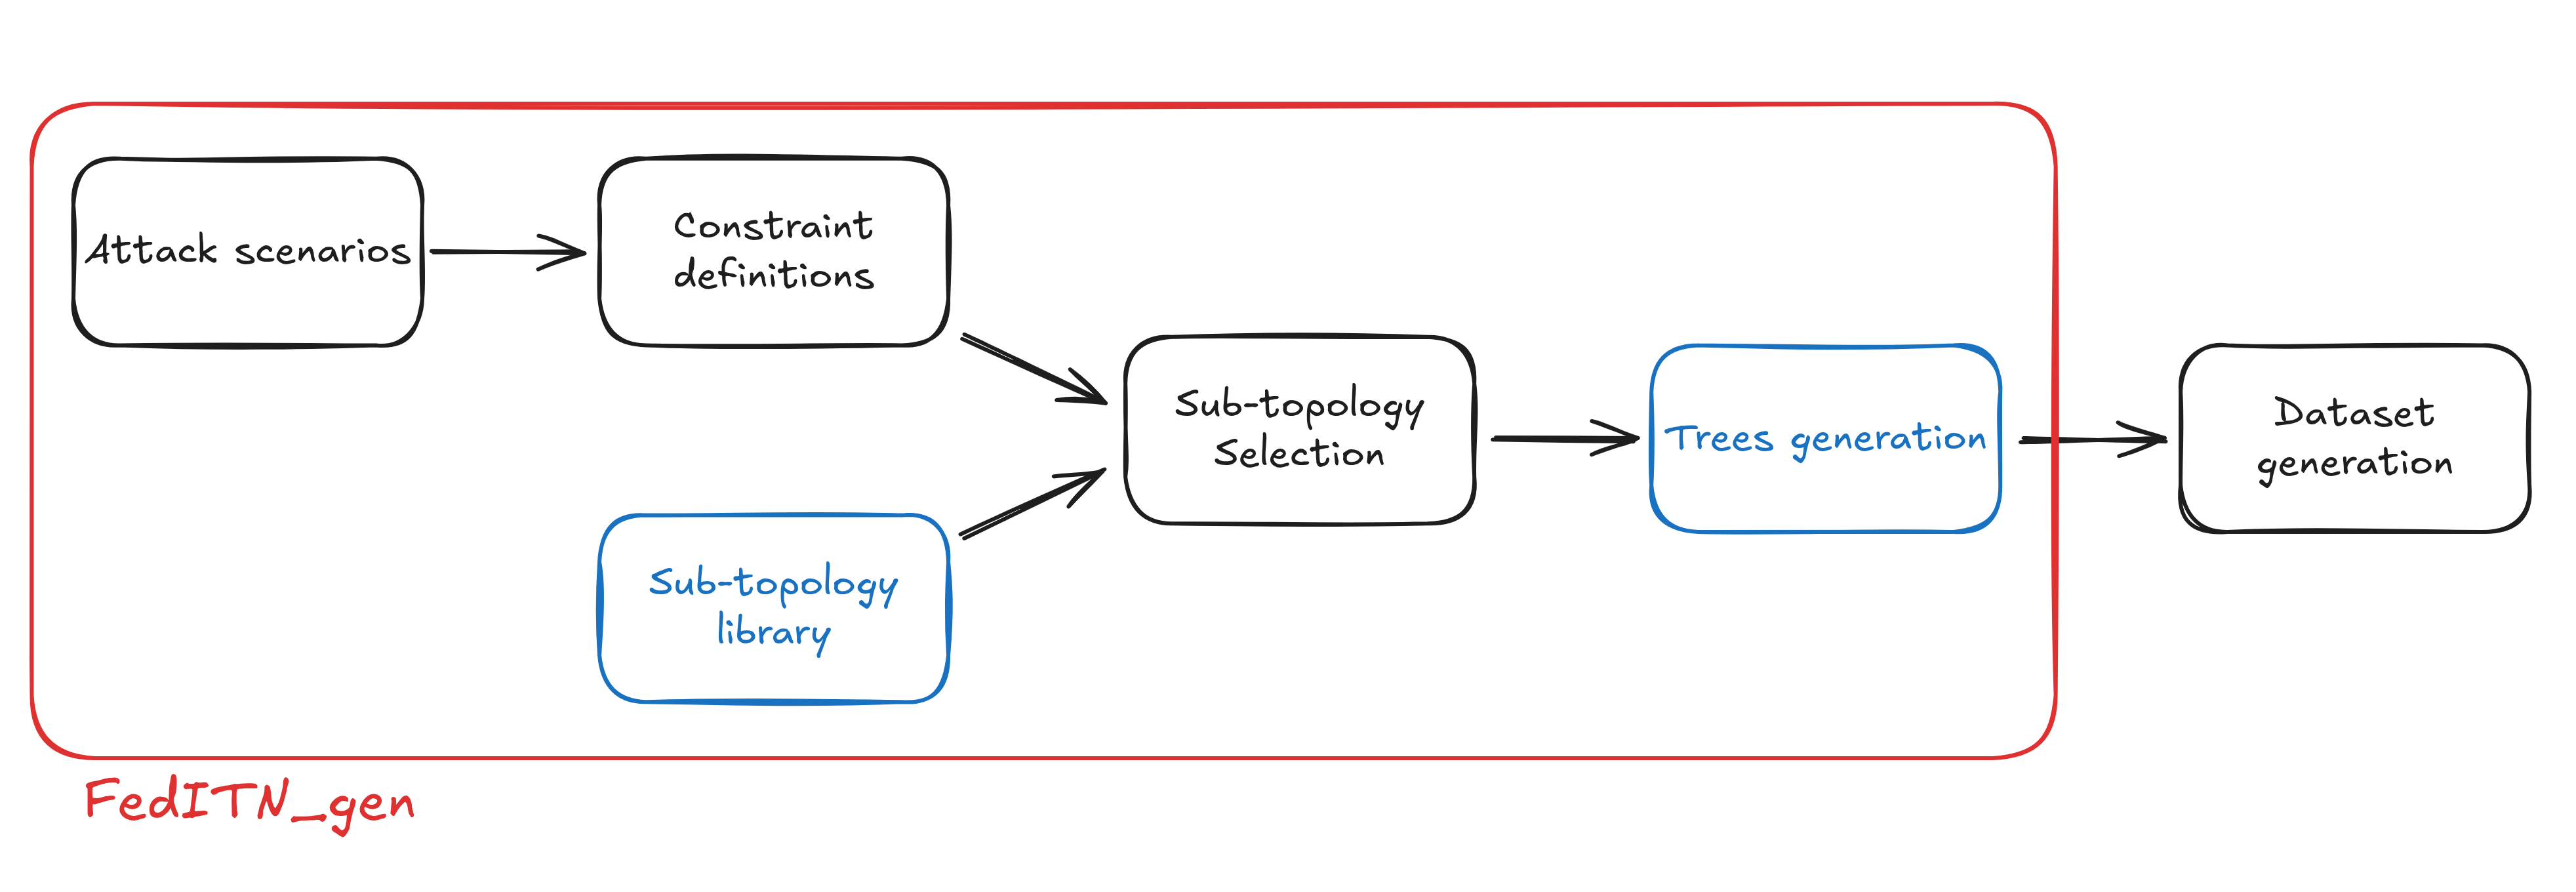
\includegraphics[width=.9\textwidth]{figures/feditn/approach/overview-topo}
\end{frame}

\begin{frame}{Sub-topologies}
  \begin{columns}
    \begin{column}{0.4\textwidth}
      \begin{figure}
        \centering
        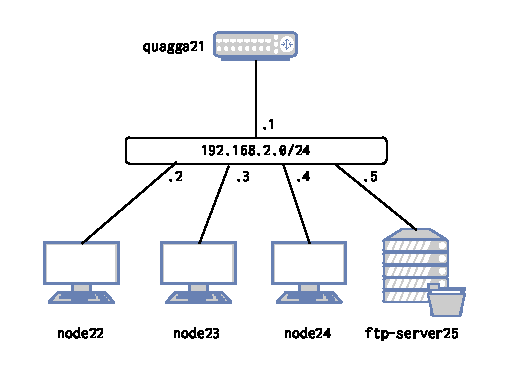
\includegraphics[width=\linewidth]{figures/feditn/approach/sub_topology.pdf}
        \caption{Example of a sub-topology with 2 types of nodes.}
      \end{figure}
    \end{column}

    \begin{column}{0.6\textwidth}
      \begin{block}{Sub-topologies}
        \begin{itemize}[<+->]
          \item Reusable building blocks;
          \item Each sub-topology has a specific role and properties (\eg, services\footnotemark, vulnerabilities);
          \item the router acts as a gateway between sub-topologies.
        \end{itemize}
      \end{block}
        
      \pause
      \begin{block}{Composition}
        \begin{itemize}[<+->]
          \item Sub-topologies are connected to form a tree (to avoid cycles);
          \item automatic routing with OSPF;
          \item the \texttt{Master} sub-topology contains the Internet gateway, the main DNS server, and DHCP/OSPF services.
        \end{itemize}
      \end{block}
    \end{column}
  \end{columns}
  \alt<2->{\footnotetext{Available services: \texttt{ldap}, \texttt{dbms}, \texttt{cms}, \texttt{dns}, \texttt{mail}, \texttt{syslog\_server}, \texttt{web}, \texttt{ftp}, \texttt{proxy}, \texttt{cloud\_storage}.}}{\only<1>{\blankfootnote{}}}

\end{frame}

\begin{frame}
  \begin{figure}
    \centering
    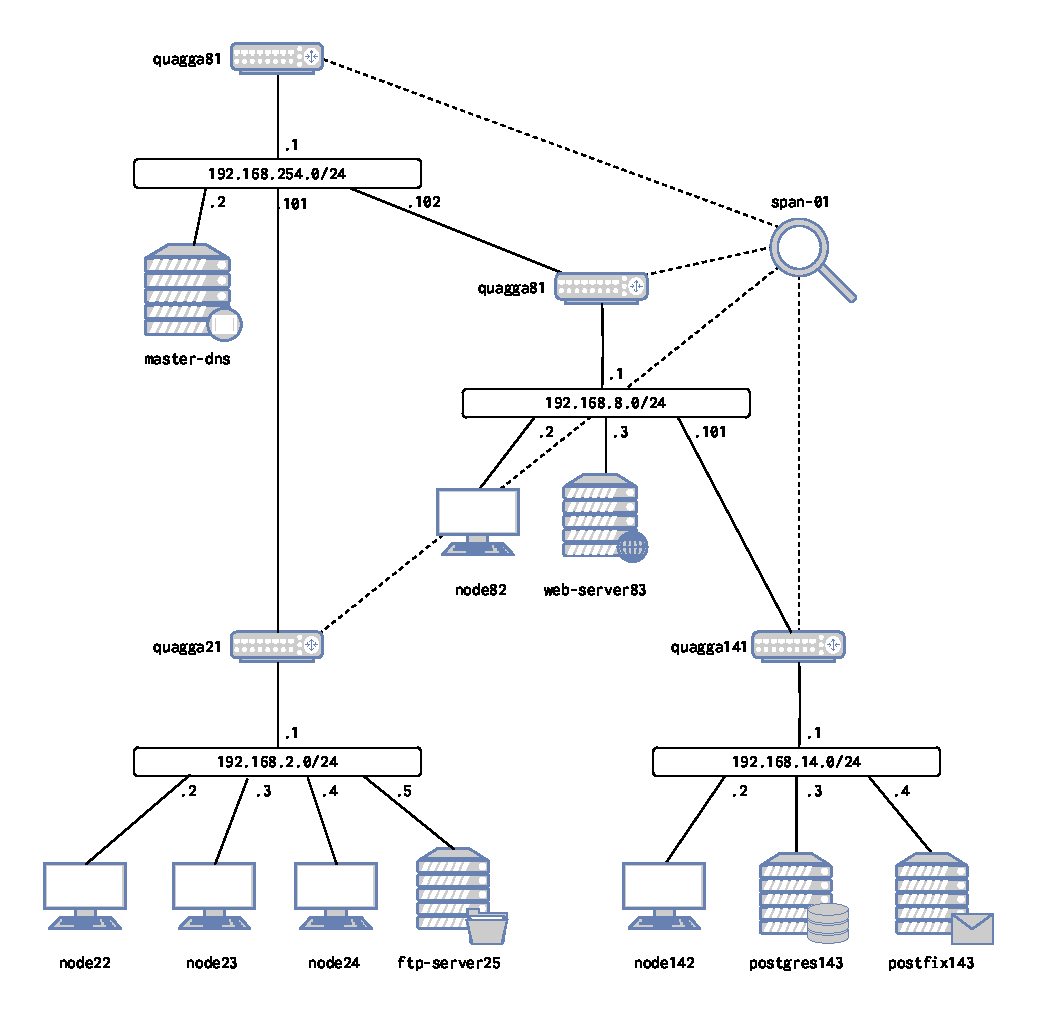
\includegraphics[height=\paperheight]{figures/feditn/approach/topology.pdf}
    \caption{Example of a generated topology with 3 sub-topologies.}
  \end{figure}
\end{frame}

      



\begin{frame}{Attack Scenarios}
  \centering
  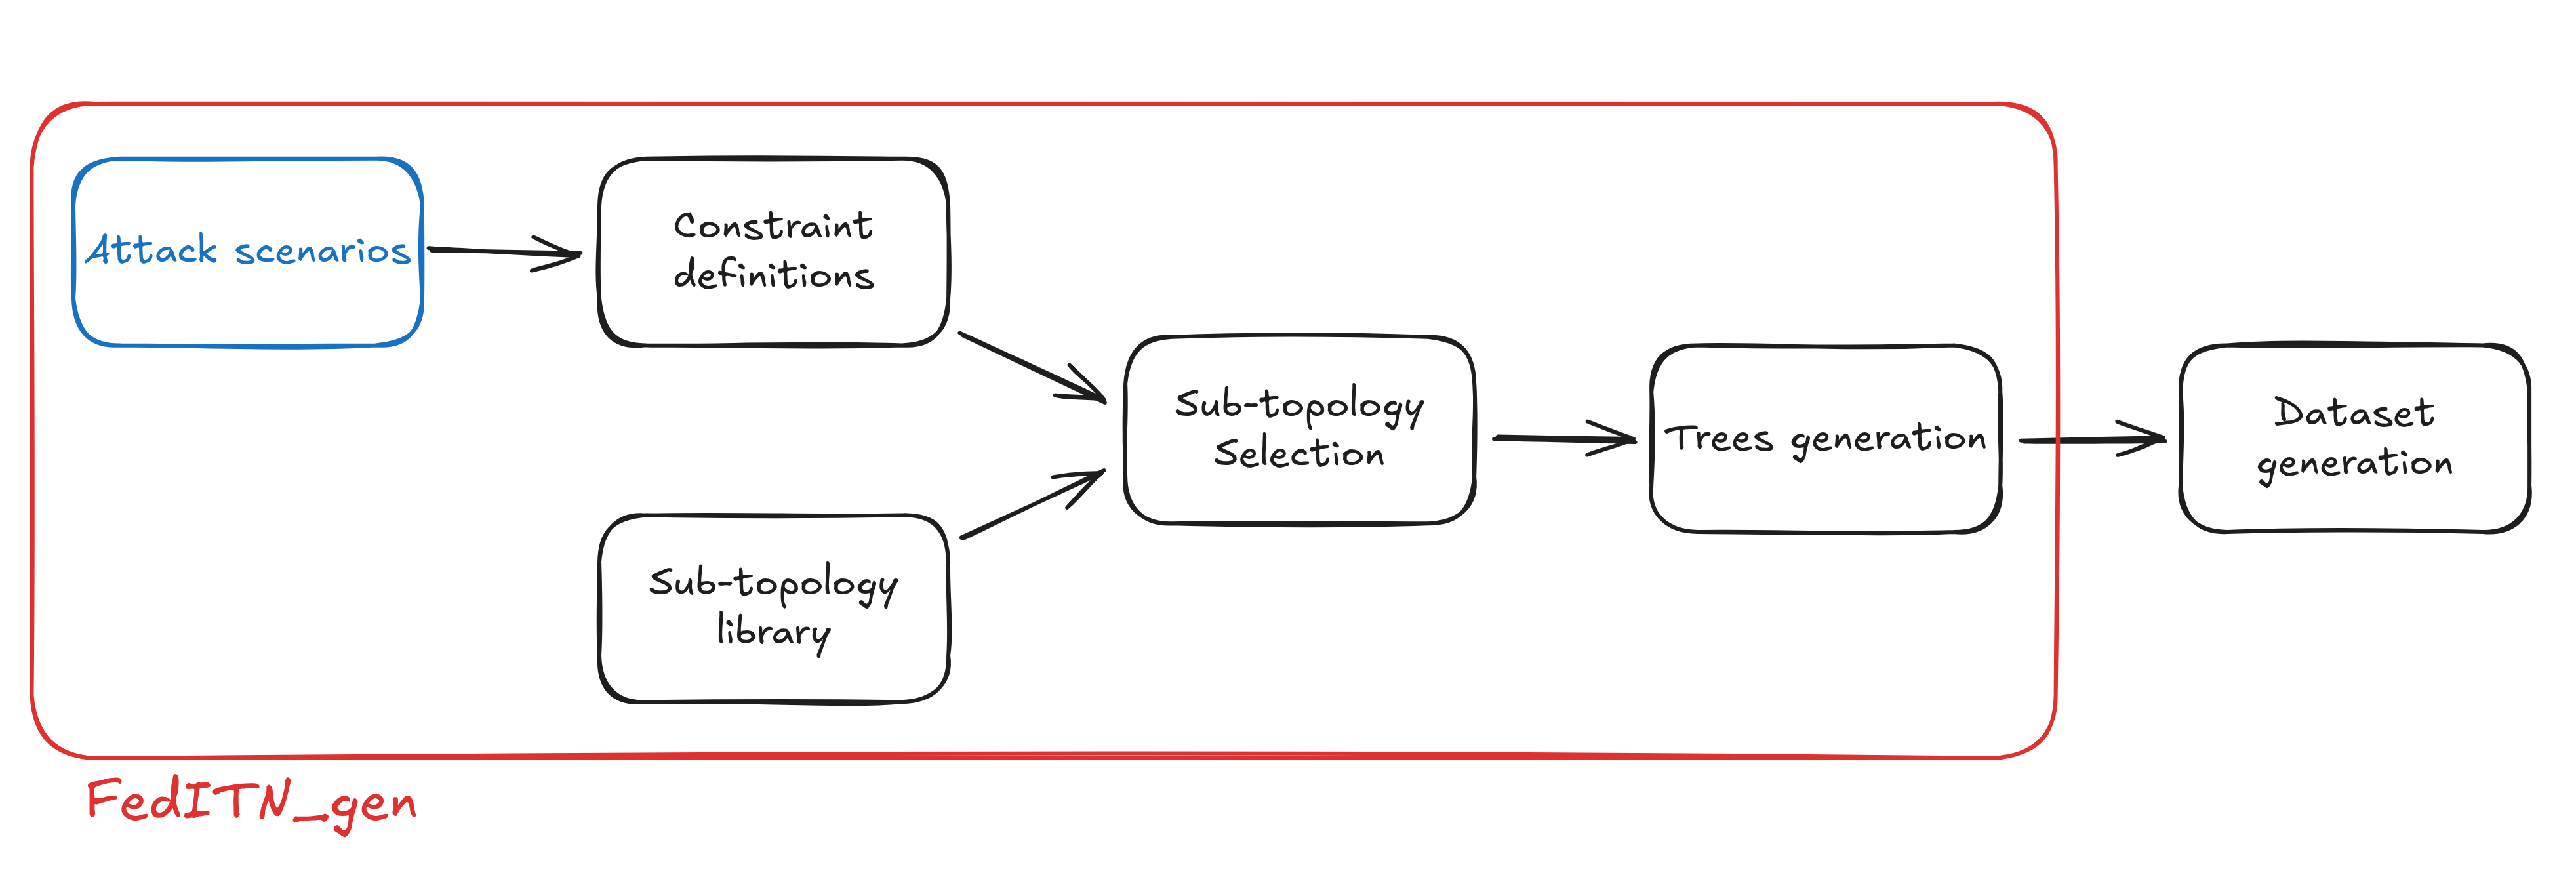
\includegraphics[width=.9\textwidth]{figures/feditn/approach/overview-attack}
\end{frame}

\begin{frame}[standout]
  \foreach \i in {1,2} {%
    \includegraphics<\i>[height=\paperheight]{figures/feditn/approach/scenario-\i}%
  }
\end{frame}


\begin{frame}{Constraint Programming}
  \centering
  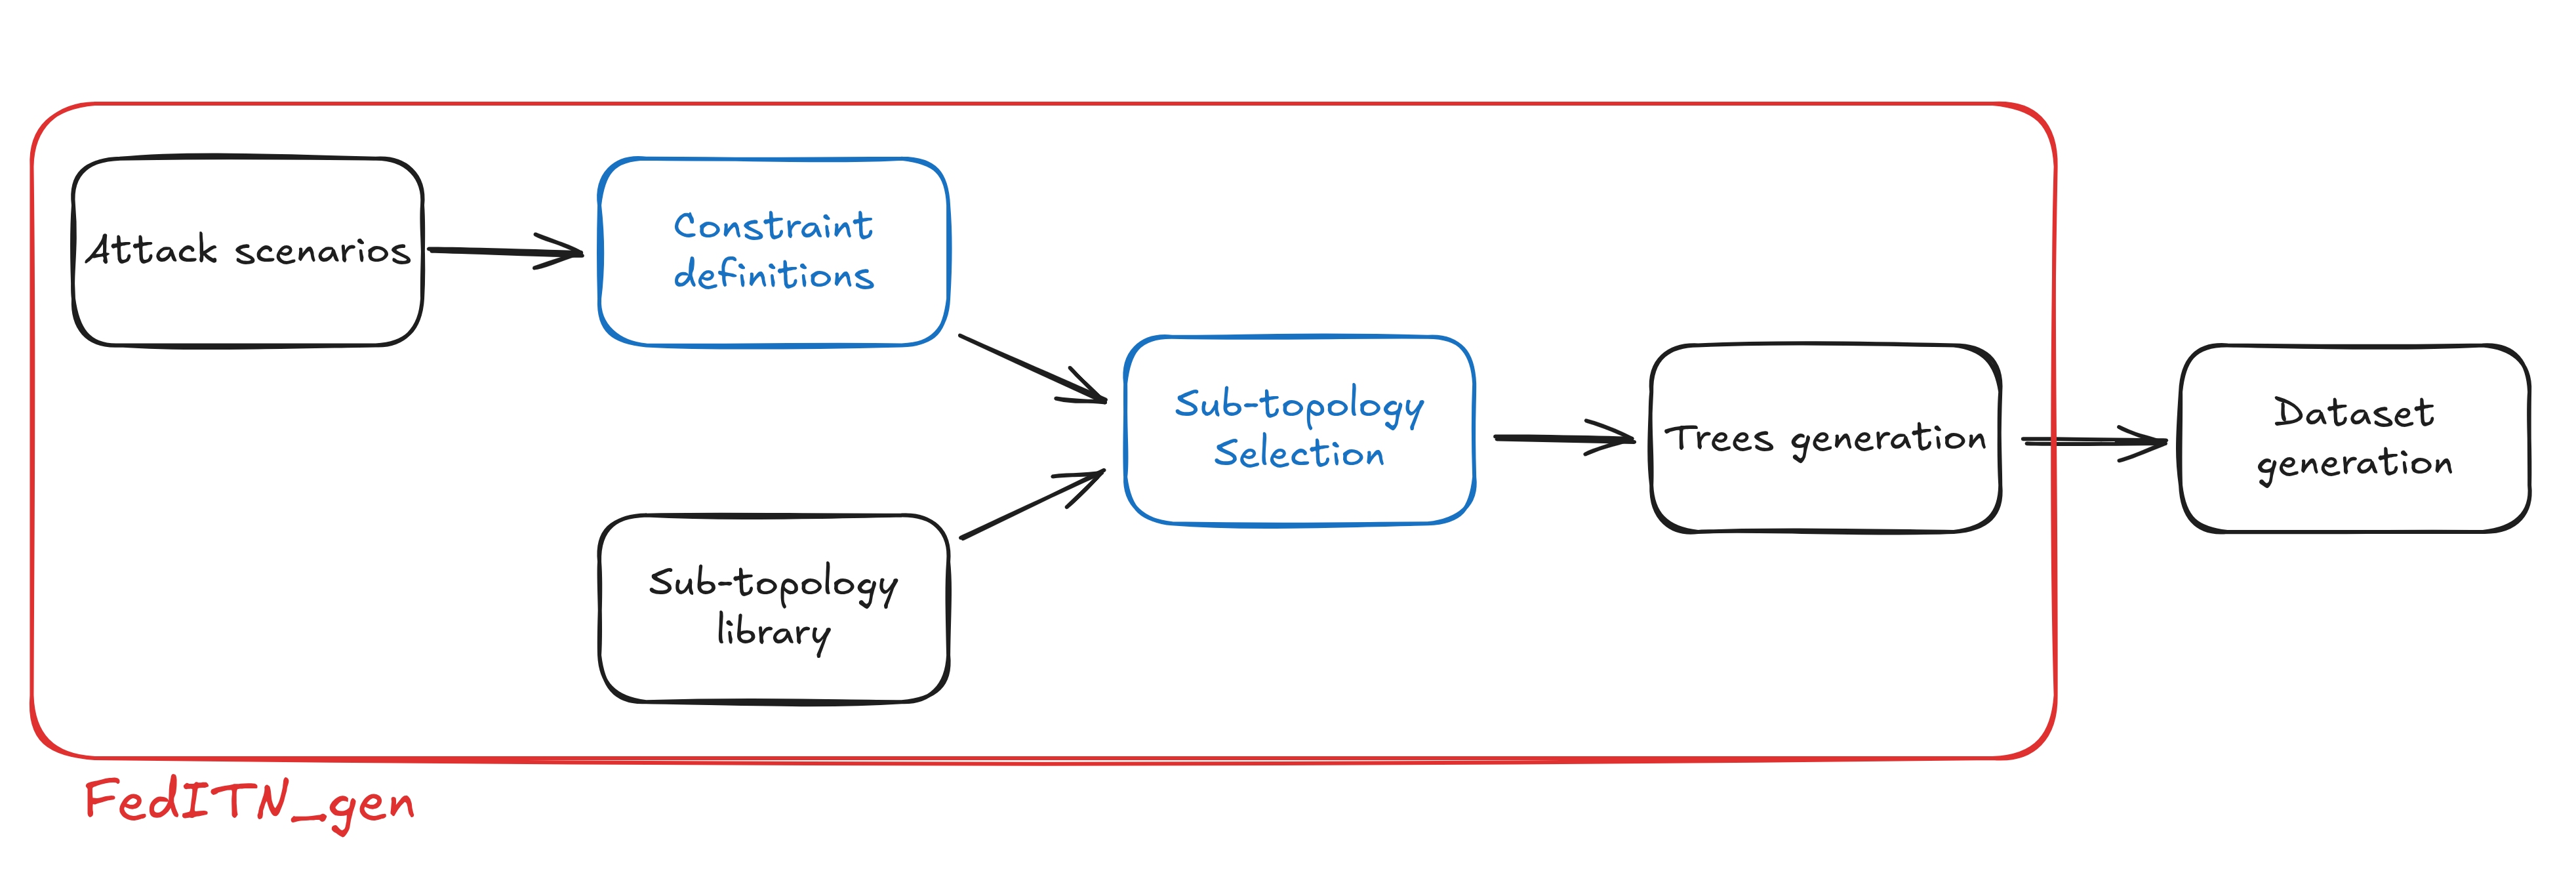
\includegraphics[width=.9\textwidth]{figures/feditn/approach/overview-constraint}
\end{frame}

\begin{frame}{Problem Formalization}
\begin{block}{Sub-topology Selection Problem (STSP)}
  \color<2->{black!30}
  Let $\mathcal{T} = \{\tau_1, \tau_2, \ldots, \tau_n\}$ be a set of sub-topologies, \textcolor<4>{sntBlue}{$D_\text{service}$ a set of services}, \textcolor<5>{sntBlue}{$A = \{a_1, a_2, \ldots, a_m\}$ a set of attack scenarios}, \textcolor<2>{sntBlue}{$k_\text{min}$ and $k_\text{max}$ the bounds of the number of subtopologies}, and \textcolor<3>{sntBlue}{$\ell_\text{min}$ and $\ell_\text{max}$ the bounds for the total number of nodes}.
  The STSP consists of finding all sets of sub-topologies $T \subseteq \mathcal{T}$ that satisfy the following:
  \begin{enumerate}
    \color<2->{black!30}
    %\normalfont
    \item \textcolor<2>{sntBlue}{$k_\text{min} \leq |T|  \leq k_\text{max}$}.
    \item \textcolor<3>{sntBlue}{$\ell_\text{min} \leq \sum\nolimits_{\tau_k \in T} | N_k| \leq \ell_\text{max}$}.
    \item \textcolor<4>{sntBlue}{$\forall s \in D_\text{service}, \exists \tau_k \in T, \text{ s.t. } s \in N_k$}.
    \item \textcolor<5>{sntBlue}{$\forall a \in A, \forall s \in a_{[\texttt{srcs}]}, \exists \tau_k \in T, \text{ s.t. } s \text{ compatible with } \tau_k$}.
    \item \textcolor<5>{sntBlue}{$\forall a \in A, \forall t \in a_{[\texttt{targets}]}, \exists \tau_k \in T, \text{ s.t. } t \text{ compatible with } \tau_k$}.
  \end{enumerate}
\end{block}
    
\end{frame}

\begin{frame}{Selection \& Composition}
  \begin{block}{Solution search}
    \begin{itemize}[<+->]
      \item Use of the CP-SAT solver from Google OR-Tools~\footnote{https://developers.google.com/optimization};
      \item The solver finds all combinations of sub-topologies satisfying the constraints;
      \item Incompatible services are pruned during the search.
      \item Trees are generated with backtracking to respect an additional depth constraint.
    \end{itemize}
  \end{block}

  \onslide<.>{\begin{figure}
    \centering
    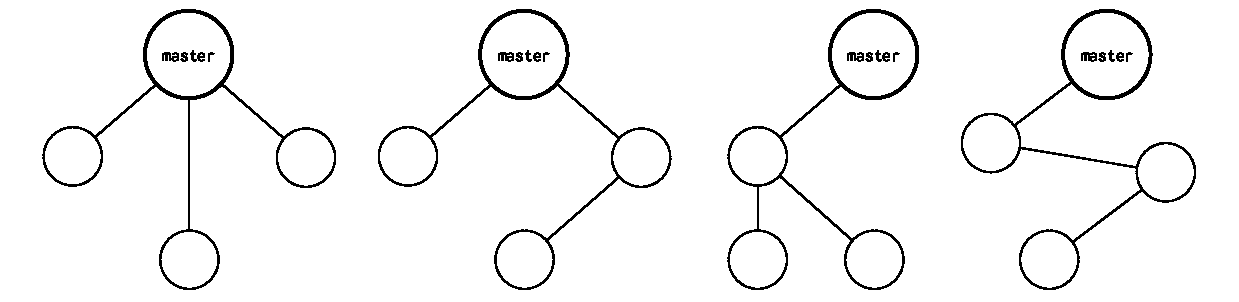
\includegraphics[width=.9\textwidth]{figures/feditn/approach/trees-3}
    \caption{Possible tree arrangements for 3 sub-topologies.}
  \end{figure}}

\end{frame}
\subsection{Takeaways on Federated Learning for Intrusion Detection}

% \begin{frame}[b]{Future Work}
%   \centering%
%   \vspace{-.3cm}
%   \foreach \i in {1,...,4} {%
%     \includegraphics<\i>[width=1.1\textwidth, center]{figures/thesis/conclusion/future/\i.pdf}%
%   }%
% \end{frame}

\begin{frame}[b]{Going beyond FIDSs}
  \centering%
  % \vspace{-.4cm}
  \foreach \i in {1,...,12} {%
    \includegraphics<\i>[width=1.05\textwidth, center, trim={0 0 0 10pt}, clip]{figures/thesis/conclusion/beyond/\i.pdf}%
  }%
\end{frame}

\begin{frame}{Is FL a good fit for collaboration?}

  \begin{block}{Yes it is!}
    \begin{itemize}
      \item Can effectively propagate knowledge on attack classes across clients~\footcite{lavaur_icdcs_demo_2024}.
      \item Specificities of the IDS use case protects it against some forms of poisoning~\eiffel.
      \item Quality and trust guarantees are possible, at the cost of scalability~\radar.
    \end{itemize}
  \end{block}

  \pause
  \begin{block}{But\dots}
    \begin{itemize}[<+->]
      \item Heterogeneity of data and objectives is a major issue~\slr; due to intrusion detection itself (\eg, complex platform-specific attack scenarios, client-specific classification).
      \item FL lacks \alert{interpretability} from both the model and the aggregation process, making deployment in sensitive environments difficult.
    \end{itemize}
  \end{block}
  % \begin{itemize}[<+->]
  %   \item Federated learning can indeed be used as a mean of collaboration for intrusion detection, but suffers from data- and objectives heterogeneity \slr. 
  %   \item It opens new attack vectors with poisoning, especially in heterogeneous settings, although bigger federation mitigate this risk \eiffel\onslide<+->; quality guarantees are possible in this setting but scale poorly \radar.
  %   \item Existing results are biased due to the lack of realistic datasets, which constraint-based generation can help mitigate \feditn. 
  %   \item Using logic reasoning over telemetry data can help link events together, but does not scale~\logic, and cannot provide confidential distributed reasoning.
  % \end{itemize}
\end{frame}

\begin{frame}{Focus on Intrusion Detection}
    \centering
    \includegraphics<+>[width=1.05\textwidth, center, trim={0 0 0 10pt}, clip]{figures/thesis/conclusion/beyond/14.pdf}%
\end{frame}
\subsection{\texorpdfstring{\logic Relationship Extraction in Distributed Events}{Relationship Extraction in Distributed Events}}

\begin{frame}{The COCTEL Project}
  \begin{block}{COCTEL: Causality-Oriented Cybersecurity TELemetry}
    \begin{itemize}
      \item \alert{Goal}: how to extract and represent relationships between events in highly distributed systems, to allow forward and backward reasoning about them.
      \item Academic project, FNR funding (Luxembourgish national research fund), PI: Jérôme François (SnT).
      \item Keywords: microservices, probabilistic logic programming, interpretable AI, explainability, causal inference.
    \end{itemize}
  \end{block}

  \tikz[overlay, remember picture]{
    \node[anchor=south east, xshift=-1em, yshift=1em] at (current page.south east) {%
      \raisebox{-0.5\height}{
\includegraphics[height=1.2cm]{assets/logos/SnT_UL_colour.pdf}}%
      \hspace{-.5em}\raisebox{-0.5\height}{
\includegraphics[height=1cm]{assets/logos/FNR_LOGO_BIG.pdf}}%
    }
  }
\end{frame}

\begin{frame}{Telemetry for tackling Partial Observability}
  \tikz[overlay, remember picture]{
    \node[anchor=north east, xshift=-1em, yshift=-3em] at (current page.north east) {%
      \raisebox{-0.5\height}{
\includegraphics[height=1.2cm]{figures/postdoc/logos/opentelemetry.png}}%
    }}

  \begin{block}{Definitions\footnotemark}
    \begin{itemize}
      \item \texttt{Telemetry} refers to the data emitted by a system.
      \item A \texttt{trace} represents the sequence of events (\texttt{span}) that occur during the execution of a request, along with their hierarchical relationships.
    \end{itemize}
  \end{block}

  \pause
  \begin{figure}
    \vspace{-1em}
    \includestandalone[width=.9\textwidth]{figures/postdoc/telemetry_waterfall.tikz}
    \caption{Waterfall representation of a trace.}
  \end{figure}

  % \begin{columns}[t]
  %   \pause
  %   \column{0.5\textwidth}
  %   \begin{block}{Advantages}
  %     \begin{itemize}
  %       \item The explicit relations provided by \emph{spans} (\ie, service call events) provide a logical structure for reasoning.
  %       \item Widely used in industry, many tools available for collection/processing.
  %     \end{itemize}
  %   \end{block}
  
  %   \pause
  %   \column{0.5\textwidth}
  %   \begin{block}{Limitations}
  %     \begin{itemize}
  %       \item Requires individual instrumentation of each service, costly.
  %       \item Operator-dependent, monitoring can be incomplete or inconsistent.
  %     \end{itemize}
  %   \end{block}
  % \end{columns}

  \footnotetext{\url{https://opentelemetry.io/docs/concepts/observability-primer/}}
\end{frame}

% \begin{frame}{Telemetry representations}
%   \begin{figure}
%     \centering
%     \only<1>{
%       \includestandalone[width=\textwidth]{figures/postdoc/telemetry_waterfall.tikz}
%       \caption{Waterfall representation of a trace.}
%     }
%     \only<2>{
%       \includestandalone[width=0.8\textwidth]{figures/postdoc/telemetry_graph.tikz}
%       \caption{Call graph for the same trace.}
%     }
%   \end{figure}
% \end{frame}

\begin{frame}[fragile]{Reasoning over Telemetry Data}
  \stepcounter{beamerpauses}
  \begin{columns}
    \column{0.5\textwidth}
    \begin{block}{Using logic programming}
      \begin{itemize}
        \item We can represent telemetry data as facts in a logic program.
        \item This allows us to perform reasoning, inference, and querying over the data.
      \end{itemize}
      \onslide<+->{Translation is easy. How can we \alert{generalize}?}
      
    \end{block}

    \column{0.5\textwidth}
    \begin{minted}[fontsize=\footnotesize]{prolog}
frontendservice("28ed4193d").
authservice("9c8a1f2b3").
 [...]
parent("28ed4193d", "9c8a1f2b3").
    \end{minted}

    \begin{minted}[fontsize=\footnotesize]{prolog}
pricingservice("34f5a6b7c").
inventoryservice("1a2b3c4d5").
 [...]
follows("34f5a6b7c", "1a2b3c4d5").
    \end{minted}
  \end{columns}
  
  \bigskip\onslide<+>
  \begin{columns}
    \column{0.5\textwidth}
    \begin{block}{Probabilistic Logic~\normalfont\autocite{raedt_ProbLogProbabilisticProlog_2007}}
      \begin{itemize}
        \item Attach probabilities to rules and facts to handle uncertainty.
      \end{itemize}
    \end{block}
    \column{0.5\textwidth}
    \begin{minted}[fontsize=\footnotesize]{prolog}
0.3::inventory_follows_cart(Inventory, Cart) :- 
  inventoryservice(Inventory),
  cartservice(Cart),
  follows(Inventory, Cart).
    \end{minted}

  \end{columns}

  \alt<.>{
  \footcite*{raedt_ProbLogProbabilisticProlog_2007}
  }{\blankfootnote{\newline}}
\end{frame}

% \begin{frame}[fragile]{Learning Logic Programs}
%   \begin{block}{Inductive Logic Programming (ILP)}
%     \begin{itemize}
%       \item Subfield of machine learning that focuses on learning logic programs from examples and background knowledge.
%       %\item Examples: FOIL (1990)~\autocite{quinlan_LearningLogicalDefinitions_1990}, Progol (1995)~\autocite{muggleton_InverseEntailmentProgol_1995}, ProbFOIL+ (2015, \emph{probabilistic})~\autocite{deraedt_InducingProbabilisticRelational_2015}, POPPER (2021)~\autocite{cropper_LearningProgramsLearning_2021a}.~*
%     \end{itemize}
%   \end{block}
%   \pause
%   \begin{columns}
%     \column{0.5\textwidth}
%     \includestandalone[width=\textwidth]{figures/postdoc/example_tree.tikz}
%     \column{0.5\textwidth}
%     \begin{block}{Example}
%       Given all \texttt{frontend}-\texttt{frontend} service pairs as positive examples of the \texttt{relation/2} predicate:
%     \end{block}
%     \medskip
%     \begin{minted}[fontsize=\footnotesize]{prolog}
% relation(V0,V1):- parent(V0,V1).
% relation(V0,V1):- follows(V0,V1).
% relation(V0,V1):- follows(V2,V1),relation(V0,V2).
%     \end{minted}
%   \end{columns}
% \end{frame}

\begin{frame}{Highlights}
  % \begin{block}{Telemetry naturally enables reasoning}
  %   Provides \alert{explicit} relationships between events, that can be used for forward and backward inference.\pause{} 
  %   Probabilistic logic can handle \alert{noisy observations} and incomplete monitoring.
  % \end{block}

  %\pause
  \begin{block}{Interpretable by design}
    Logic programs are \alert{human-readable} and can be easily integrated with LLMs for querying and generation.
  \end{block}

  \pause
  \begin{block}{Generalizes well to intrusion detection}
    Logic relationships can be used to represent complex attack patterns, including \alert{existing knowledge} (\eg, MITRE ATT\&CK).
  \end{block}
\end{frame}

\begin{frame}{Using Logic for Model Adaptation}
  \begin{itemize}[<+->]
    \item Neural-symbolic AI combines symbolic reasoning or representation with neural networks.
    \item Logic programs can be used to guide or modify the output of a neural model, allowing for \alert{model adaptation} without retraining.
  \end{itemize}

  \onslide<+->
  \begin{table}
    \centering
    \caption{Fixing misclassification issues in CasinoLimit~\autocite{kilian_CasinoLimitOffensiveDataset_2025} by adding contextual logic rules using Scallop.
    Macro-F1 on the targeted instances.}
    \small
    \begin{tabular}{llll}
      \toprule
      \textbf{Row} & \textbf{Ping (\texttt{ligolo-ng})} & \textbf{Grep (\texttt{linpeas.sh})} & \textbf{Combined} \\
      \midrule
      Baseline & 0.423277 & 0.423277 & 0.423277 \\
      Logic at inference & 0.455895 (+7.71\%) & 0.488943 (+15.51\%) & 0.521561 (+23.22\%) \\
      KL Distillation & 0.438017 (+3.48\%) & 0.533949 (+26.15\%) & 0.555552 (+31.25\%) \\
      Logic at training & 0.444519 (+5.02\%) & 0.560168 (+32.34\%) & 0.618868 (-46.21\%) \\
      %Relabelling & 0.444132 (+4.93\%) & 0.585468 (+38.32\%) & 0.697962 (+64.89\%) \\
      \bottomrule
    \end{tabular}
  \end{table}

  \alt<3>{\footcite*{kilian_CasinoLimitOffensiveDataset_2025}}{\blankfootnote{}}
\end{frame}


\section{Conclusion}

\begin{frame}{What about collaboration?}
  \stepcounter{beamerpauses}

  \begin{block}{Client-specific objectives}
    \textit{Learn globally, then adapt locally.} Facilitate collaboration while respecting client-specific constraints.
  \end{block}

  \pause
  \begin{block}{Federated Logic Programs Learning}
    Multiple clients could collaboratively learn a shared logic program, akin to FL. 
    \pause{} With what aggregation function?
    \pause{} What impact from heterogeneity? 
    \pause{} What about poisoning?
  \end{block}

  \pause
  \begin{block}{Allowing distributed reasoning}
    Logic programs might hold too much semantics to be shared (privacy concerns).\pause{} $\Rightarrow$ Use federated learning to learn a shared embedding space for logic predicates, allowing for \alert{confidential} distributed reasoning.
  \end{block}


  %   \begin{itemize}[<+->]
  %     \item Problem: Logic programs might be too explicit to be shared (privacy concerns due to semantic richness)\dots \onslide<+->\emph{inapplicable to federated learning?}.
  %     \item Solution: use distributed representation learning to learn a shared embedding space for logic predicates, allowing for \alert{confidential} distributed reasoning.
  %   \end{itemize}
  % \end{block}
  
\end{frame}

\begin{frame}{Where to?}
  \centering
  \includegraphics<+>[width=1.05\textwidth, trim={0 0 0 10pt}, clip]{figures/thesis/conclusion/beyond/12.pdf}%
  \includegraphics<+->[width=1.05\textwidth, trim={0 0 0 10pt}, clip]{figures/project.drawio.pdf}%

  \onslide<+->
  \begin{tikzpicture}[remember picture,overlay]
    \node[
      anchor=north west,
      yshift=-3em,
      fill=white, fill opacity=0.85, text opacity=1,
      text width=.7\textwidth,
      align=left,
      inner sep=.8em
    ] at (current page.north west) {%
      \small
      \textbf{Collaborative \alert{neural-symbolic} reasoning}
      \begin{itemize}
        \item<4-> \alert{Simpler} (federated) learning objectives, which are more robust to heterogeneity and poisoning.
        \item<5-> Use logic reasoning for \alert{interpretable} decision-making, with distributed representation learning to provide \alert{confidential} entity resolution across organizations.
      \end{itemize}
    };
  \end{tikzpicture}
\end{frame}


\begin{frame}{Where to?}
  \stepcounter{beamerpauses}
  \begin{block}{\centering Collaborative \alert{neural-symbolic} reasoning}
    \begin{itemize}
      \item \alert{Simpler} (federated) learning objectives, which are more robust to heterogeneity and poisoning.
      \item Use logic reasoning for \alert{interpretable} decision-making, with distributed representation learning to provide \alert{confidential} entity resolution across organizations.
      %\item Pursue the development of \alert{independent} datasets.
    \end{itemize}
  \end{block}

  \bigskip\centering\rule{.4\textwidth}{.4pt}
  
  \medskip\Large \alert{Thank you!}
  
  \medskip\normalfont\tt
  leo.lavaur@uni.lu | leolavaur.re

\end{frame}


\appendix

\begin{frame}[allowframebreaks]{References}
    \printbibliography[heading=none]
\end{frame}

\section*{Backup slides}

\begin{frame}
  \sectionpage
\end{frame}



\subsection{\S~Assessment Study}

\begin{frame}{Predictability}
  \begin{figure}
    \centering
    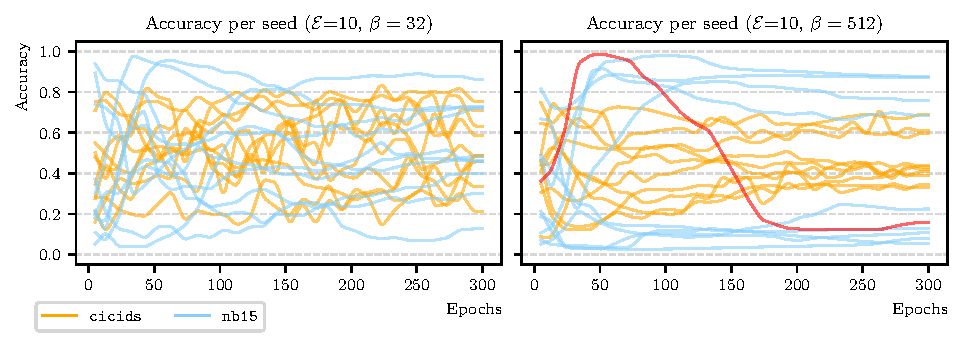
\includegraphics[width=0.8\textwidth]{figures/thesis/assessment/accuracy_per_seed.pdf}
    \caption{Accuracy of a FIDS under attack, across different random seeds.}
  \end{figure}
\end{frame}

\begin{frame}{Impact on attack propagation}
  \begin{figure}
    \centering
    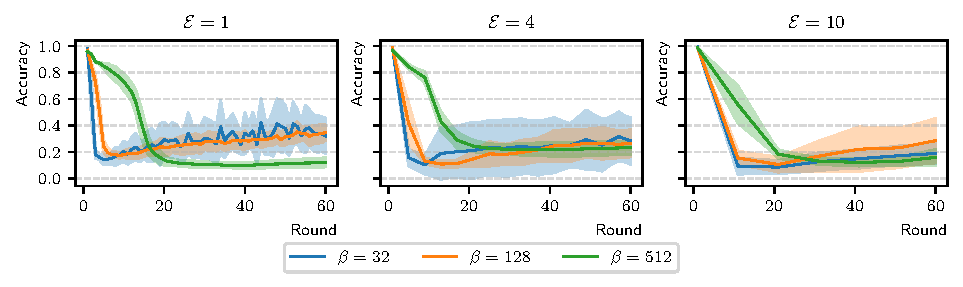
\includegraphics[width=0.8\textwidth]{figures/thesis/assessment/hyperparams-late-icdcs.pdf}
    \caption{Accuracy across rounds for different batch sizes.}
  \end{figure}  
\end{frame}

\subsection{\S~Neural-symbolic AI}

\begin{frame}{\texttt{Scallop}}
  \begin{figure}
    \centering
    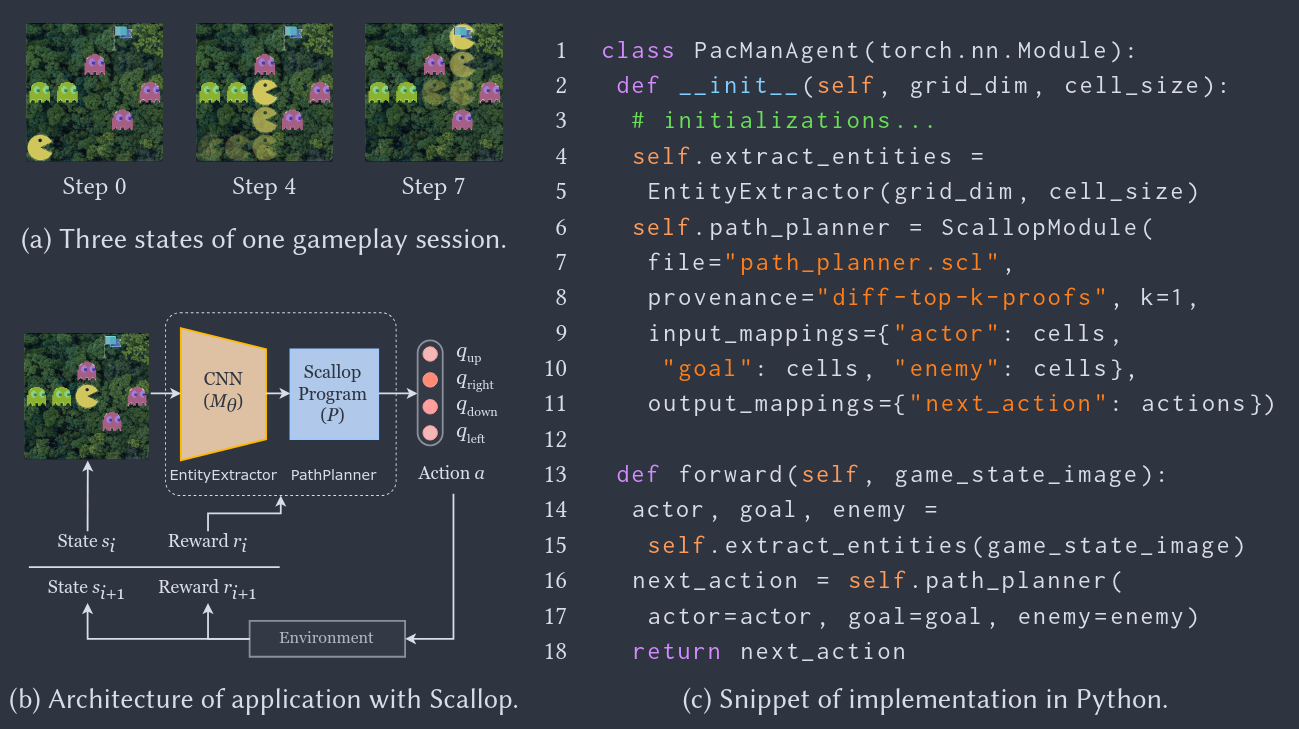
\includegraphics[width=0.75\textwidth]{figures/postdoc/scallop_appendix.png}
    \caption{Scallop~\footcite{huang_ScallopProbabilisticDeductive_2021}.}
  \end{figure}
\end{frame}

\begin{frame}{\texttt{DeepProbLog}}
  \begin{figure}
    \centering
    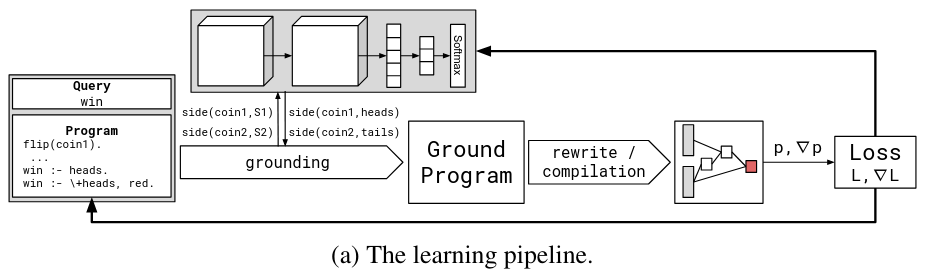
\includegraphics[width=0.8\textwidth]{figures/postdoc/deepproblog_appendix.png}
    \caption{DeepProbLog~\footcite{manhaeve_DeepProbLogNeuralProbabilistic_2018}.}
  \end{figure}
\end{frame}

\subsection{\S~\tt FedITN\_gen}

\section{FedITN}

\begin{frame}{Project definition}
  \begin{block}{Objective}
  Design a systematic approach to generate \emph<+>{deployable} network topologies, capable of producing \emph<+>{heterogeneous} and \emph<+>{independent} datasets for evaluating Federated Intrusion Detection Systems (FIDSs).
  \end{block}

  \pause
  \begin{block}{Requirements}
    \begin{itemize}[<+->]
      \item \emph{diversity} in topologies, attacks and devices to provide heterogeneity;
      \item approach \emph{realism} in terms of traffic and behaviors;
      \item \emph{controllable} data distribution across clients;
      \item data \emph{independence} amongst clients;
    \end{itemize}
  \end{block}
\end{frame}

% \begin{frame}{Related work}
%   \begin{columns}[t]
%     \begin{column}{.33\textwidth}
%       \begin{block}{Protocol testing~\autocite{doar_bettermodelgenerating_1996,medina_BRITEapproachuniversal_2001}}
%         \begin{itemize}
%           \item Internet-like topologies, not applicable to enterprise networks;
%           \item focus on structural properties or degree distributions (\eg, power-law).
%         \end{itemize}
%       \end{block}
%     \end{column}
%     \onslide<+(1)->
%     \begin{column}{.33\textwidth}
%       \begin{block}{Usecase or task focused}
%         \begin{itemize}[<+->]
%           \item Declarative topology generation (\eg, \texttt{TopoGen}~\autocite{laurito_TopoGennetworktopology_2017} for SDN);
%           \item Layer-based composition for Industrial Control Networks (\eg, \texttt{GENIND}~\autocite{alrumaih_GENINDindustrialnetwork_2023});
%         \end{itemize}
%       \end{block}
%     \end{column}
    
%     \onslide<.(1)->
%     \begin{column}{.33\textwidth}
%       \begin{block}{Cyber-ranges}
%         \begin{itemize}[<+->]
%           \item Declarative deployments of scenarios and topologies~\autocite{venkatesan_VulnerVANVulnerableNetwork_2019,yamin_Modelingexecutingcyber_2022};
%           \item Vulnerable environment generation from attack graphs (\eg, \texttt{URSID}~\autocite{besson_URSIDAutomaticallyRefining_2024a}).
%         \end{itemize}
%       \end{block}
%     \end{column}
%   \end{columns}

%   \only<1>{\footcite*{doar_bettermodelgenerating_1996,medina_BRITEapproachuniversal_2001}}
%   \only<2-3>{\footcite*{laurito_TopoGennetworktopology_2017}}
%   \alt<3>{\footcite*{alrumaih_GENINDindustrialnetwork_2023}}{\only<2>{\blankfootnote{}\blankfootnote{}}}
%   \only<4-5>{\footcite*{venkatesan_VulnerVANVulnerableNetwork_2019}}
%   \alt<5>{\footcite*{yamin_Modelingexecutingcyber_2022}}{\only<4>{\blankfootnote{}\blankfootnote{}}}
  

% \end{frame}

\begin{frame}{FedITN Approach Overview}
  % attack scenarios -> constraints -> compatible subtopologies -> topology trees
  \centering
  \includegraphics<1>[width=.9\textwidth]{figures/feditn/approach/overview-1}%
  \includegraphics<2>[width=.9\textwidth]{figures/feditn/approach/overview-2}%
\end{frame}

\begin{frame}{Topology composition}
  \centering
  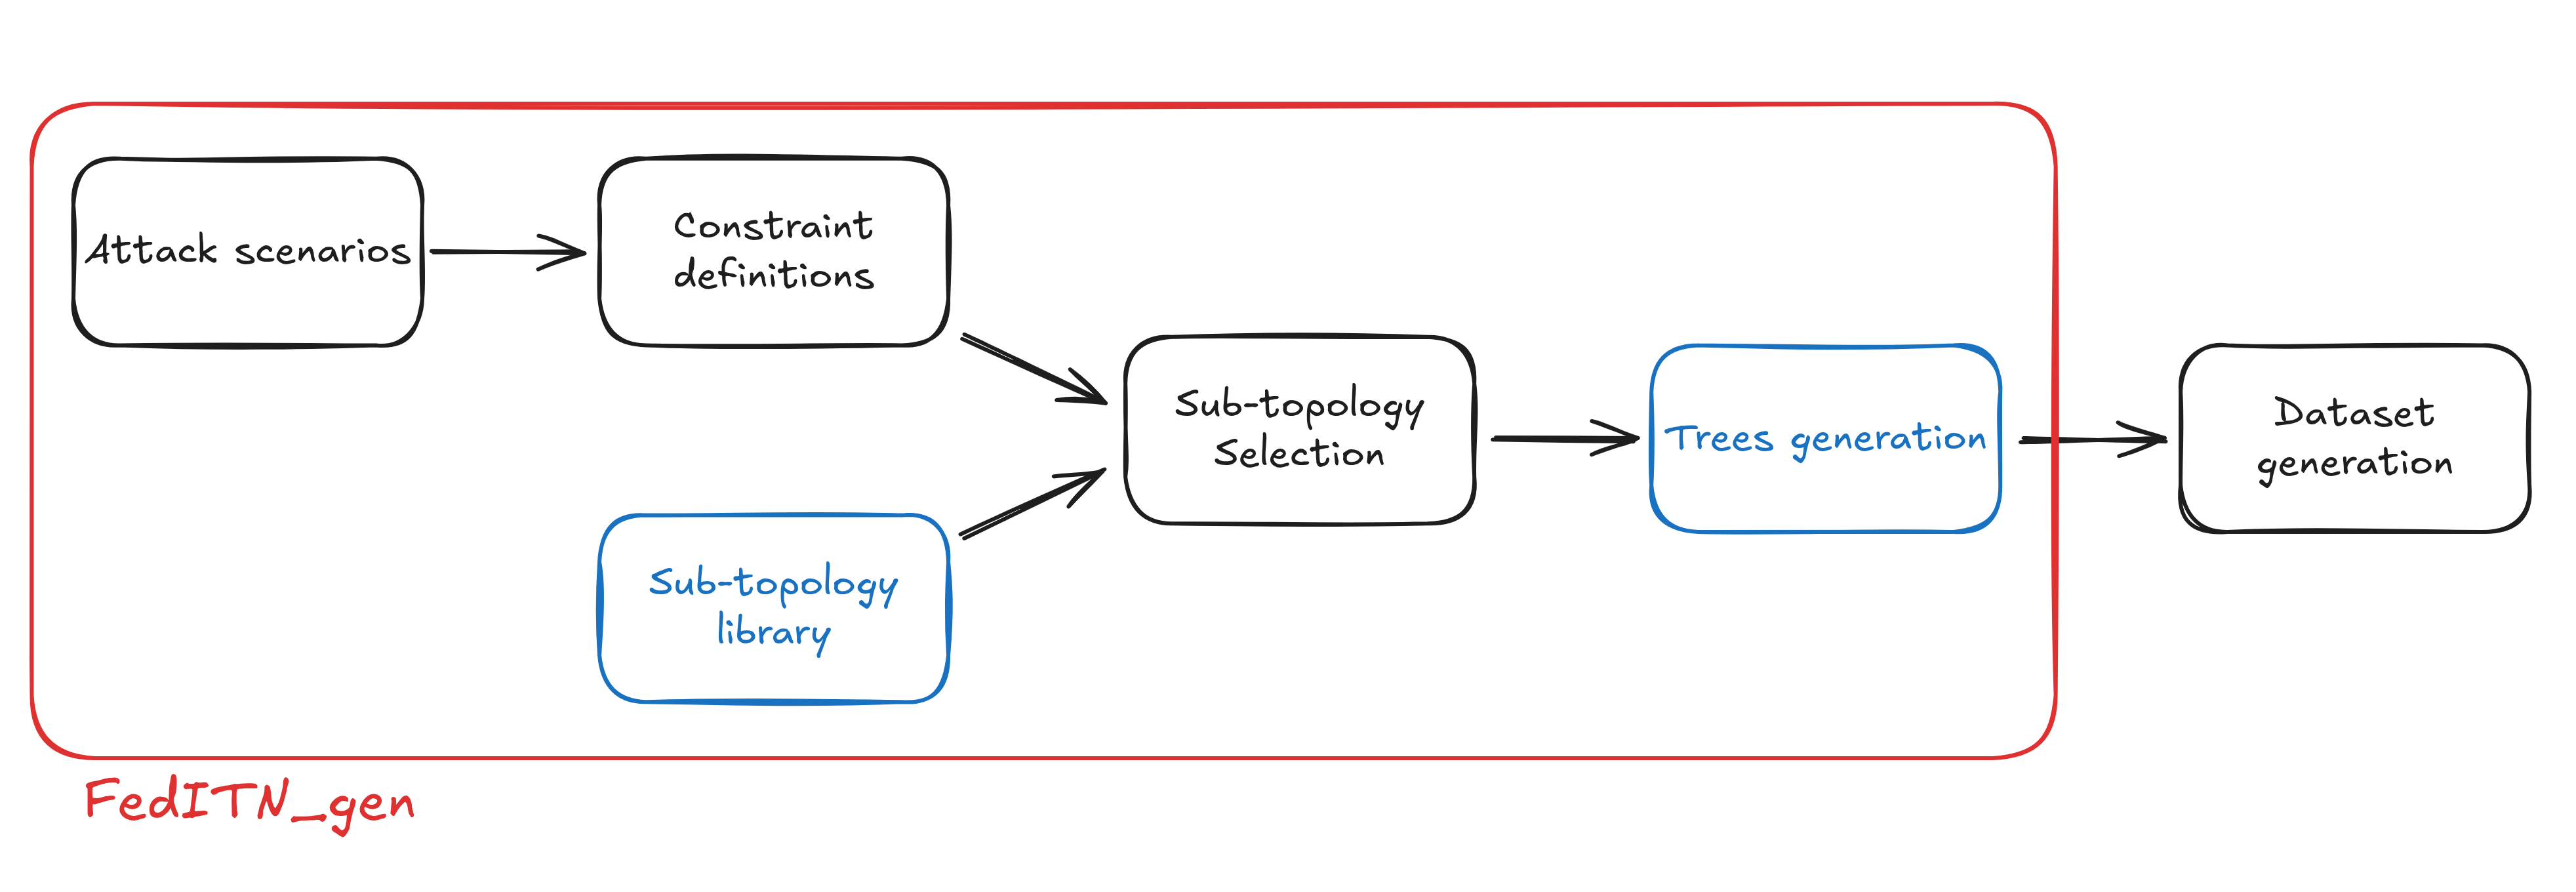
\includegraphics[width=.9\textwidth]{figures/feditn/approach/overview-topo}
\end{frame}

\begin{frame}{Sub-topologies}
  \begin{columns}
    \begin{column}{0.4\textwidth}
      \begin{figure}
        \centering
        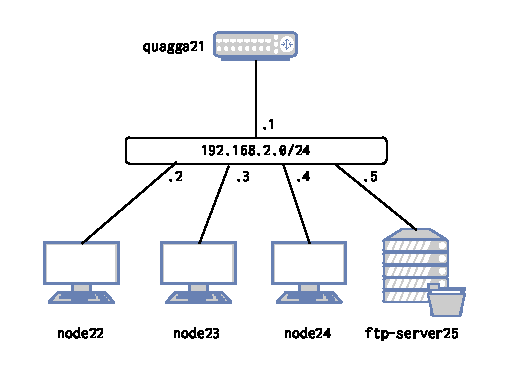
\includegraphics[width=\linewidth]{figures/feditn/approach/sub_topology.pdf}
        \caption{Example of a sub-topology with 2 types of nodes.}
      \end{figure}
    \end{column}

    \begin{column}{0.6\textwidth}
      \begin{block}{Sub-topologies}
        \begin{itemize}[<+->]
          \item Reusable building blocks;
          \item Each sub-topology has a specific role and properties (\eg, services\footnotemark, vulnerabilities);
          \item the router acts as a gateway between sub-topologies.
        \end{itemize}
      \end{block}
        
      \pause
      \begin{block}{Composition}
        \begin{itemize}[<+->]
          \item Sub-topologies are connected to form a tree (to avoid cycles);
          \item automatic routing with OSPF;
          \item the \texttt{Master} sub-topology contains the Internet gateway, the main DNS server, and DHCP/OSPF services.
        \end{itemize}
      \end{block}
    \end{column}
  \end{columns}
  \alt<2->{\footnotetext{Available services: \texttt{ldap}, \texttt{dbms}, \texttt{cms}, \texttt{dns}, \texttt{mail}, \texttt{syslog\_server}, \texttt{web}, \texttt{ftp}, \texttt{proxy}, \texttt{cloud\_storage}.}}{\only<1>{\blankfootnote{}}}

\end{frame}

\begin{frame}
  \begin{figure}
    \centering
    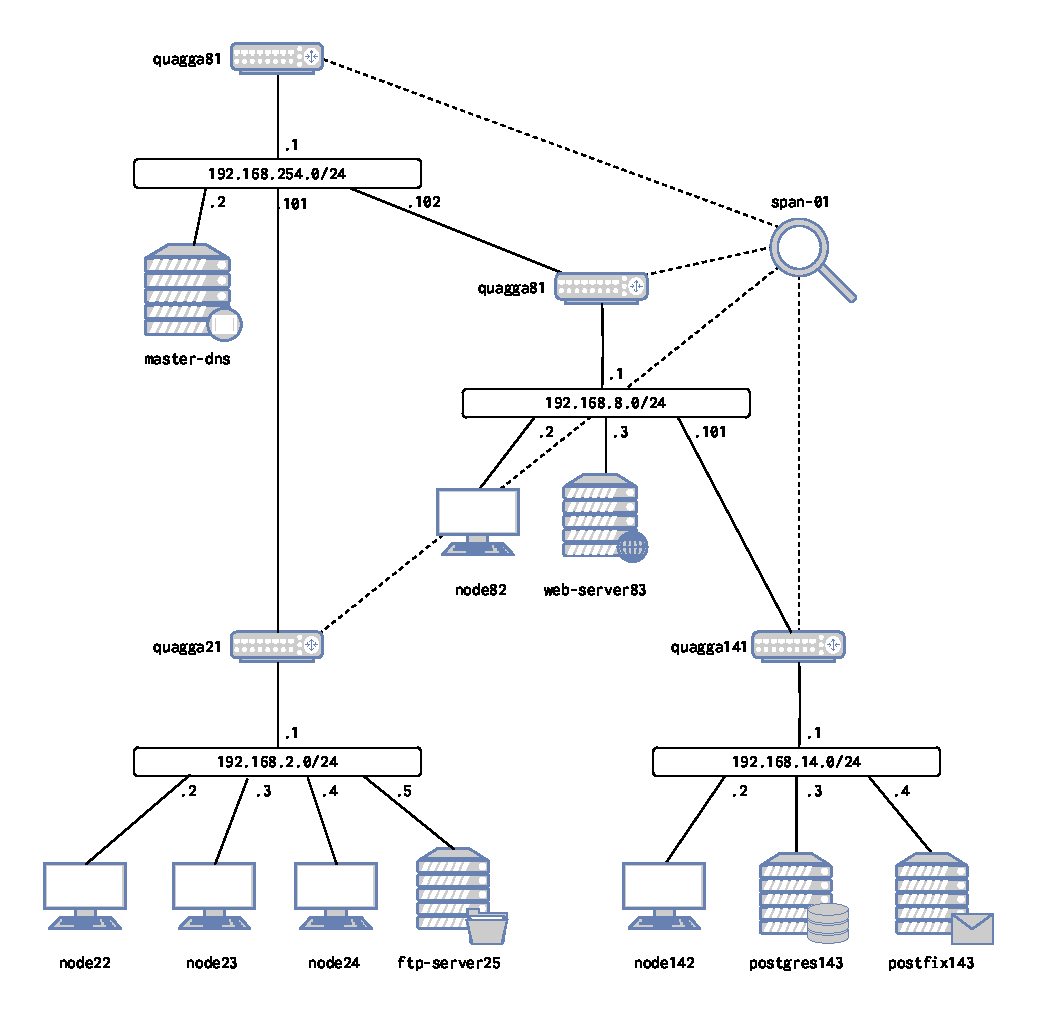
\includegraphics[height=\paperheight]{figures/feditn/approach/topology.pdf}
    \caption{Example of a generated topology with 3 sub-topologies.}
  \end{figure}
\end{frame}

      



\begin{frame}{Attack Scenarios}
  \centering
  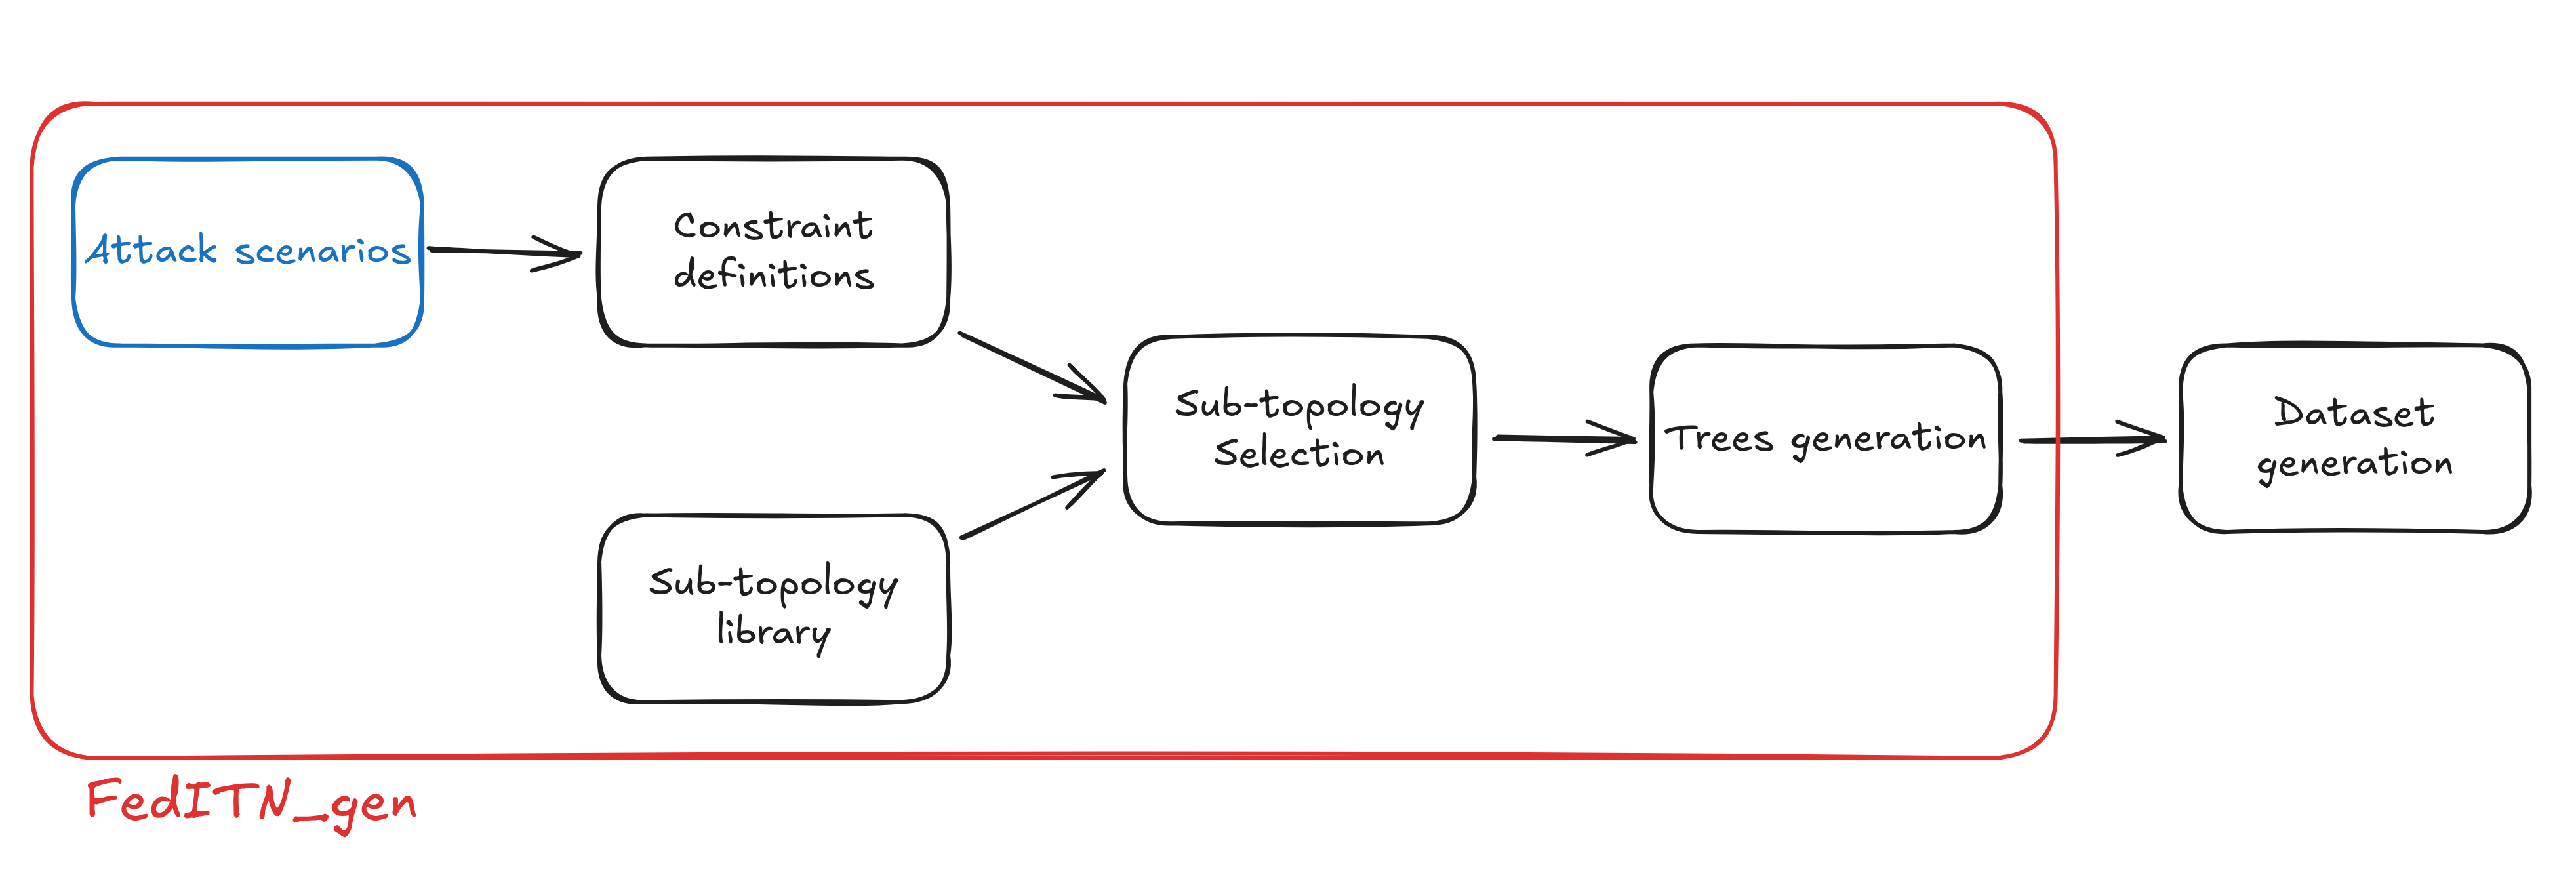
\includegraphics[width=.9\textwidth]{figures/feditn/approach/overview-attack}
\end{frame}

\begin{frame}[standout]
  \foreach \i in {1,2} {%
    \includegraphics<\i>[height=\paperheight]{figures/feditn/approach/scenario-\i}%
  }
\end{frame}


\begin{frame}{Constraint Programming}
  \centering
  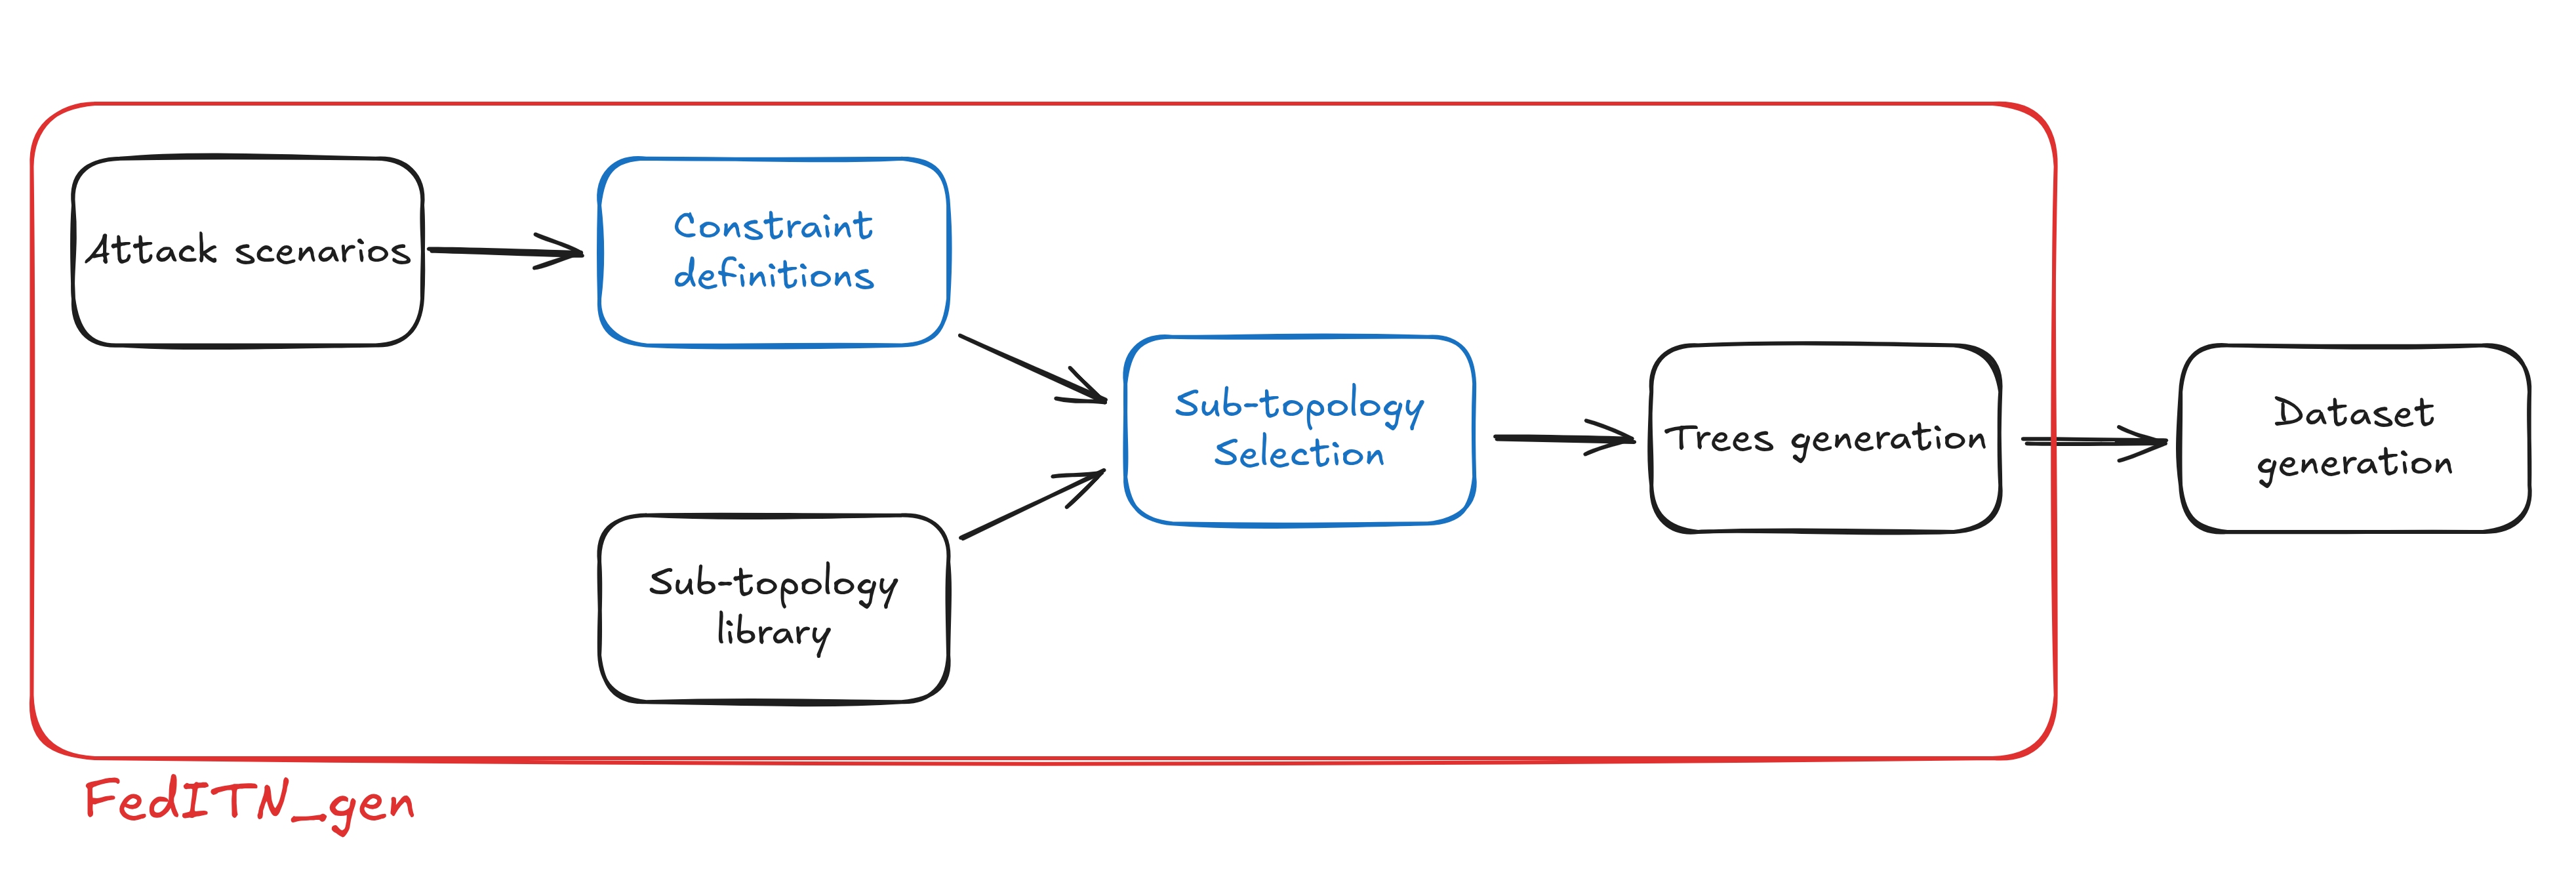
\includegraphics[width=.9\textwidth]{figures/feditn/approach/overview-constraint}
\end{frame}

\begin{frame}{Problem Formalization}
\begin{block}{Sub-topology Selection Problem (STSP)}
  \color<2->{black!30}
  Let $\mathcal{T} = \{\tau_1, \tau_2, \ldots, \tau_n\}$ be a set of sub-topologies, \alert<4>{$D_\text{service}$ a set of services}, \alert<5>{$A = \{a_1, a_2, \ldots, a_m\}$ a set of attack scenarios}, \alert<2>{$k_\text{min}$ and $k_\text{max}$ the bounds of the number of subtopologies}, and \alert<3>{$\ell_\text{min}$ and $\ell_\text{max}$ the bounds for the total number of nodes}.
  The STSP consists of finding all sets of sub-topologies $T \subseteq \mathcal{T}$ that satisfy the following:
  \begin{enumerate}
    \color<2->{black!30}
    %\normalfont
    \item \alert<2>{$k_\text{min} \leq |T|  \leq k_\text{max}$}.
    \item \alert<3>{$\ell_\text{min} \leq \sum\nolimits_{\tau_k \in T} | N_k| \leq \ell_\text{max}$}.
    \item \alert<4>{$\forall s \in D_\text{service}, \exists \tau_k \in T, \text{ s.t. } s \in N_k$}.
    \item \alert<5>{$\forall a \in A, \forall s \in a_{[\texttt{srcs}]}, \exists \tau_k \in T, \text{ s.t. } s \text{ compatible with } \tau_k$}.
    \item \alert<5>{$\forall a \in A, \forall t \in a_{[\texttt{targets}]}, \exists \tau_k \in T, \text{ s.t. } t \text{ compatible with } \tau_k$}.
  \end{enumerate}
\end{block}
    
\end{frame}

\begin{frame}{Selection \& Composition}
  \begin{block}{Solution search}
    \begin{itemize}[<+->]
      \item Use of the CP-SAT solver from Google OR-Tools~\footnote{https://developers.google.com/optimization};
      \item The solver finds all combinations of sub-topologies satisfying the constraints;
      \item Incompatible services are pruned during the search.
      \item Trees are generated with backtracking to respect an additional depth constraint.
    \end{itemize}
  \end{block}

  \onslide<.>{\begin{figure}
    \centering
    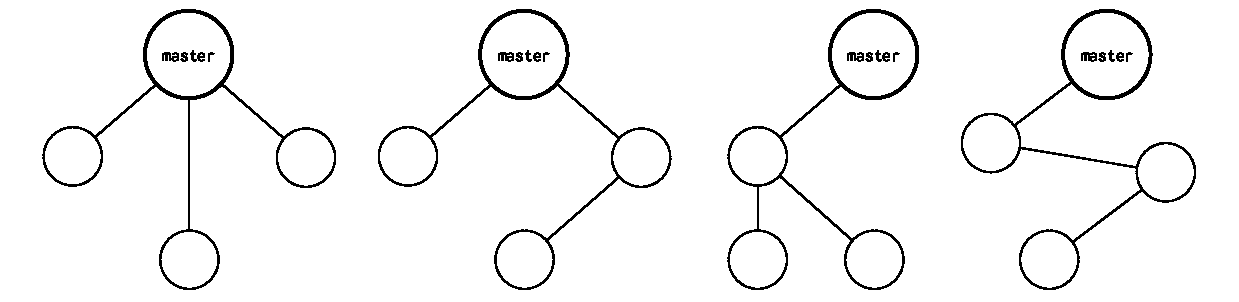
\includegraphics[width=.9\textwidth]{figures/feditn/approach/trees-3}
    \caption{Possible tree arrangements for 3 sub-topologies.}
  \end{figure}}

\end{frame}

\end{document}
